%% thesis.tex 2014/04/11
%
% Based on sample files of unknown authorship.
%
% The Current Maintainer of this work is Paul Vojta.

\documentclass{ucbthesis}
%\usepackage{biblatex}
\usepackage{natbib} % use natbib over biblatex to be able to use GSAB .bst
\usepackage{textcomp,marvosym}
\usepackage{amsmath,amssymb}
\usepackage{rotating} % provides sidewaystable and sidewaysfigure
\usepackage{graphicx}
\usepackage{xspace}
\usepackage[hidelinks]{hyperref}
\urlstyle{same}
\usepackage{threeparttable}
\usepackage[font=footnotesize,format=plain,labelfont=bf,up,textfont=up]{caption} % change figure caption style
\usepackage{color,colortbl}
%\usepackage[table,xcdraw]{xcolor}
\usepackage{sidecap}
\usepackage{bibentry}
\usepackage{multirow}
\usepackage{pdfpages}
\bibliographystyle{gsabull}

% To compile this file, run "latex thesis", then "biber thesis"
% (or "bibtex thesis", if the output from latex asks for that instead),
% and then "latex thesis" (without the quotes in each case).

% Double spacing, if you want it.  Do not use for the final copy.
% \def\dsp{\def\baselinestretch{2.0}\large\normalsize}
% \dsp

% If the Grad. Division insists that the first paragraph of a section
% be indented (like the others), then include this line:
% \usepackage{indentfirst}

\addtolength{\abovecaptionskip}{\baselineskip}

\newtheorem{theorem}{Jibberish}


\begin{document}
% Declarations for Front Matter

\title{Late Proterozoic magmatism, geodynamo, and paleogeography from Laurentian paleomagnetic records}
\author{Yiming Zhang}
\degreesemester{Spring}
\degreeyear{2024}
\degree{Doctor of Philosophy}
\chair{Professor Nicholas L. Swanson-Hysell}
\othermembers{Professor Bruce A. Buffett \\
   Professor Seth Finnegan}
\numberofmembers{3}

\field{Earth \& Planetary Science}


\maketitle
% Delete (or comment out) the \approvalpage line for the final version.
%\approvalpage
\copyrightpage

% (This file is included by thesis.tex; you do not latex it by itself.)

\begin{abstract}

% \begin{center}
%     \textit{``An ancient time\\
%     When compass needles lost their way; \\
%     Finding North from South." \\}
%     \vspace{10pt}
%     S. W. Bogue
% \end{center}

Over 2000 years ago, one of humanity's earliest records of harnessing magnetism unfolded in ancient China, where lodestones (i.e. magnetic rocks) were used in telling directions in geomancy and divination practices. Compass made its way to Europe through the Silk Road, which granted European mariners the ability to tell their heading regardless of weather conditions or visibility constraints at sea. The improved navigation for mariners contributed to the Age of Discovery. Scientific advances through the following centuries have made profound insights into the fundamental principles of electromagnetism. Today, our continued understanding and manipulation of the electromagnetic principles lie at the core of modern technology and life. 

It is because compass needles are made of magnetic materials that tend to align with Earth's magnetic field at surface which is dominantly dipolar and stable such that a compass can help navigate today. In the rock records, there are numerous microscopic compasses that are carrying ancient magnetic records through deep time. These microscopic compasses are magnetic minerals such as iron-titanium oxides and iron sulfides that occur rather ubiquitously in igneous, sedimentary, and metamorphic rocks. Being rooted in understanding of rock forming processes and the physics of electromagnetism, the study of paleomagnetism utilizes these magnetic compasses in rocks to explore Earth history topics.

In this dissertation, I find my applications of paleomagnetism in revealing the characteristics of magmatism in the Midcontinent Rift system in the Lake Superior region and in the southwestern Laurentia 1.1 billion years ago, shedding new lights in the strength of the geodynamo ca. 1092 million years ago, and furthering the development of global paleogeography through the end of the Mesoproterozoic and the earliest Neoproterozoic. 

\subsection{Late Mesoproterozoic magmatism in the Midcontinent Rift and the southwestern Laurentia large igneous province}

The ancient North American craton, Laurentia, first formed in the Paleoproterozoic Era when a series of collisional orogenies culminating the Trans-Hudson orogeny led to the amalgamation of Archean provinces \citep{Hoffman1988a, Whitmeyer2007a}. The craton continued to grow through the rest of the Paleoproterozoic and into the Mesoproterozoic via accretionary orogenesis along its margin. In the latest Mesoproterozoic (ca. 1110 to 1080 Ma) the large intracontinental Midcontinent Rift, which was co-located with a large igneous province (LIP) \citep{Swanson-Hysell2021a} led to extension within the Archean Superior province and adjacent Paleoproterozoic provinces to the south \citep{Cannon1992a}. Protracted magmatic activities punctuated by rapid and voluminous emplacement of extrusive and intrusive rocks in the rift led to the emplacement of a thick succession of volcanic rocks and mafic intrusions in Laurentia’s interior. Syn- to post-rift thermal subsidence led to deposition of clastic sedimentary rocks on top of the igneous rocks.

\begin{figure}[h!]
    \centering
    \includegraphics[width=0.9\textwidth]{figure/chapters_overview.pdf}
    \caption{(A) Simplified map of North America showing the areal extent of the 1.1 Ga Midcontinent Rift and the southwestern Laurentia large igneous province. The inset boxes show the extent of areas of study of the dissertation chapters. (B) Compilation of chemical abrasion-isotope dilution-thermal ionization mass spectrometry (CA-ID-TIMS) zircon U-Pb geochronology data from the Midcontinent Rift and southwestern Laurentia. Data are from \citep{Fairchild2017a, Swanson-Hysell2014a, Swanson-Hysell2019a, Mohr2024a}. The colored zones represent the estimated duration of the pulsed and voluminous magmatic events in Laurentia ca. 1.1 Ga.}
    \label{fig:overview}
\end{figure}

The Midcontinent Rift eventually ceased and failed to split the continent into two. Far-field compressional forces associated with the onset and development of the Grenvillian orogeny along the eastern margin of Laurentia led to cessation and subsequent inversion of the rift \citep{Cannon1993a, Swanson-Hysell2019a}. In the southern Lake Superior region, Midcontinent Rift volcanic and sedimentary rocks were uplifted along with Paleoproterozoic and Archean lithologies via thrust faults, forming the crustal-scale Montreal River monocline \citep{Cannon1993a}. The resultant topography led to the deposition of the early Neoproterozoic Jacobsville Formation \citep{Hamblin1958a, Kalliokoski1982a, Hodgin2022a}, which overlies an angular unconformity that developed on lithologies that were exhumed through this earlier episode of contractional deformation associated with Grenvillian orogenesis. 

The intracontinental nature of the rift and the its cessation led to large amount of rift rocks being preserved in the interior of Laurentia far from continental margins. Rocks in the rift were subsequently experienced mild burial and metamorphism history. Rb-Sr dates from the uplifted basement rocks in southern Lake Superior region show that the area has not been heated to above 300 \textdegree C since ca. 1050 Ma \citep{Cannon1993a}. $^{10}$Be data show that some surface bedrock exposures have only recently been near the surface due to Pleistocene glacial and recent fluvial erosion \cite[e.g.][]{Ullman2015a}. 

The rich record of well-preserved Midcontinent Rift rocks provide a wealth of opportunities for characterizing the magmatic history of Laurentia at the time. Geochronology and geochemistry data have been used to divide magmatic activity in the rift into four stages based on interpreted changes in relative magmatic volume and the nature of magmatism: early ($\sim$1109--1104 Ma), latent ($\sim$1104--1098 Ma), main ($\sim$1098--1090 Ma) and late ($\sim$1090--1083 Ma) \citep{Vervoort2007a, Heaman2007a, Miller2013a}. Advances in the method of chemical abrasion-isotope dilution-thermal ionization mass spectroscopy (CA-ID-TIMS) and its application in obtaining high-precision zircon U-Pb ages, together with the development of high-quality paleomagnetic data from the extrusive and intrusive rocks, have revealed distinct rapid and voluminous episodes of magmatism in the rift during the overall protracted period of active magmatism \citep{Swanson-Hysell2019a, Swanson-Hysell2021a, Zhang2021b}. In particular, a large igneous province, consisting of the massive Duluth Complex and its associated $\sim$8 km thick extrusive lava flows of the North Shore Volcanic Group, formed within 500 Kyr ca. 1096 Ma \citep{Swanson-Hysell2021a}. Stratigraphically above the Duluth Complex, the ca. 1092 Ma mafic Beaver Bay Complex represents another rapid and voluminous pulse of magmatism. It features the emplacement of the hypabyssal intrusion of the Beaver River diabase that has wide magma conduits containing giant anorthosite xenoliths that can be as much as 300 meters in width. Unlike the Duluth Complex and the North Shore Volcanic Group, whose magmatic linkage is supported by the exposed stratigraphic relationships and geochronologic data, there is no direct exposure of volcanic rocks that overlie conformably on top of the Beaver River diabase. Previously on the basis of geochemical data and petrographic observations, a hypothesis was put forward that the Greenstone Flow of the Portage Lake Volcanics that outcrop in the upper Keweenaw Peninsula in Michigan could be the surface expression of the Beaver River diabase. In chapter 1, I test this hypothesis by using paleomagnetic and geochronologic data to investigate the synchroneity of the emplacement of the intrusive and extrusive rocks. The data support that the Beaver River diabase was the feeder system for the $\sim$400 meters thick Greenstone Flow which ranks one of the largest lava flows known on Earth. In chapter 2, I utilize the exceptionally well-preserved anorthosite xenoliths hosted in the Beaver River diabase to shed new light on the evolution of Earth's geodynamo.

While rapid and voluminous mafic magmatism occurred in the Midcontinent Rift, improved geochronologic and paleomagnetic data show that distinct episodes of mafic magmatism occurred in southwestern Laurentia ca. 1098 Ma and ca. 1082 Ma \citep{Mohr2024a}. During a period of $<$0.25 Myr ca. 1098 Ma, thick mafic diabase sills and dikes intruded through southwestern basement rocks into the Mesoproterozoic sedimentary rocks including the Crystal Spring Formation in the Death Valley, Unkar Group sedimentary rocks in the Grand Canyon, and the Apache Group sedimentary rocks in central Arizona \citep{Bright2014a}. The tempo and extent of this episode of mafic magmatism and juvenile geochemical signature of the rocks are consistent with there being a southwestern large igneous province driven by a mantle plume. That the emplacement of the voluminous intrusions in the southwest occurred 2 Myr prior to the Duluth Complex led \citep{Mohr2024a} to invoke a tectonic model, where the mantle plume first arrived ca. 1098 Ma in southwestern Laurentia and laterally transported toward the readily thinned crust of the Midcontinent Rift. The arrival of the plume material in the rift postdates the latent magmatic stage ($\sim$1104--1098 Ma) and led to a replenishment of mafic magma and heat supply in the rift, which eventually drove the emplacement of the ca. 1096 Ma Duluth Complex and the associated lava flows. In chapter 3 I develop new paleomagnetic data from southwestern Laurentia and update the extent of the southwestern large igneous province. 

The Grenvillian orogenesis is a major event leading up to the assembly of the supercontinent Rodinia with Laurentia at its center \citep{Swanson-Hysell2023a}. Magmatism waned in the Midcontinent Rift and Laurentia's plate speed slowed down as the continental-scale collision commenced along Laurentia's eastern margin \citep{Swanson-Hysell2019a}. Following this time, there has been a lack of magmatism in Lauretia and thus a lack of well-dated paleomagnetic data that constrains global paleogeography until Rodinia began to rift apart $\sim$300 Myr later \citep{Eyster2019a}. The deposition of the post-rift Jacobsville Formation has been dated to be ca. 990 Ma and thus provides an opportunity to constrain the position of Rodinia in the earliest Neoproterozoic. In chapter 4 I develop new paleomagnetic data from the Jacobsville Formation in a detailed stratigraphic context. 

\subsection*{The GAD hypothesis in the late Mesoproterozoic}

Earth's magnetic field today is dominated by the dipole component \citep{Alken2021a}. It is the working hypothesis that the surface expression of Earth’s geomagnetic field in deep time averages out to a geocentric axial dipole (GAD) whose poles coincides with the geographic poles that grants power to paleomagnetic directional observations. In the GAD model, an observation of an inclination of magnetization (I) uniquely corresponds to a latitude value ($\lambda$). This direction-pole relationship is expressed in the ``dipole equation" 
\begin{equation}
    tan(I) = 2 tan(\lambda)
\label{direction_eq}
\end{equation} The GAD hypothesis also empowers paleomagnetic field intensity observations in that there is a unique correspondence between an observed field strength at any latitude and the axial dipole moment, which is mathematically expressed as 
\begin{equation}
    H = \frac{M\sqrt{1+3cos^2\theta}}{r^3}
\label{intensity_eq}
\end{equation} Where H is the observed magnetic field intensity, M is the magnetic moment of Earth, $\theta$ is colatitude where $\theta=90-\lambda$, and r is Earth's radius. 

% add inclination-latitude figure and geomagnetic field-dipole moment strength paired plot
\begin{figure}[h!]
    \centering
    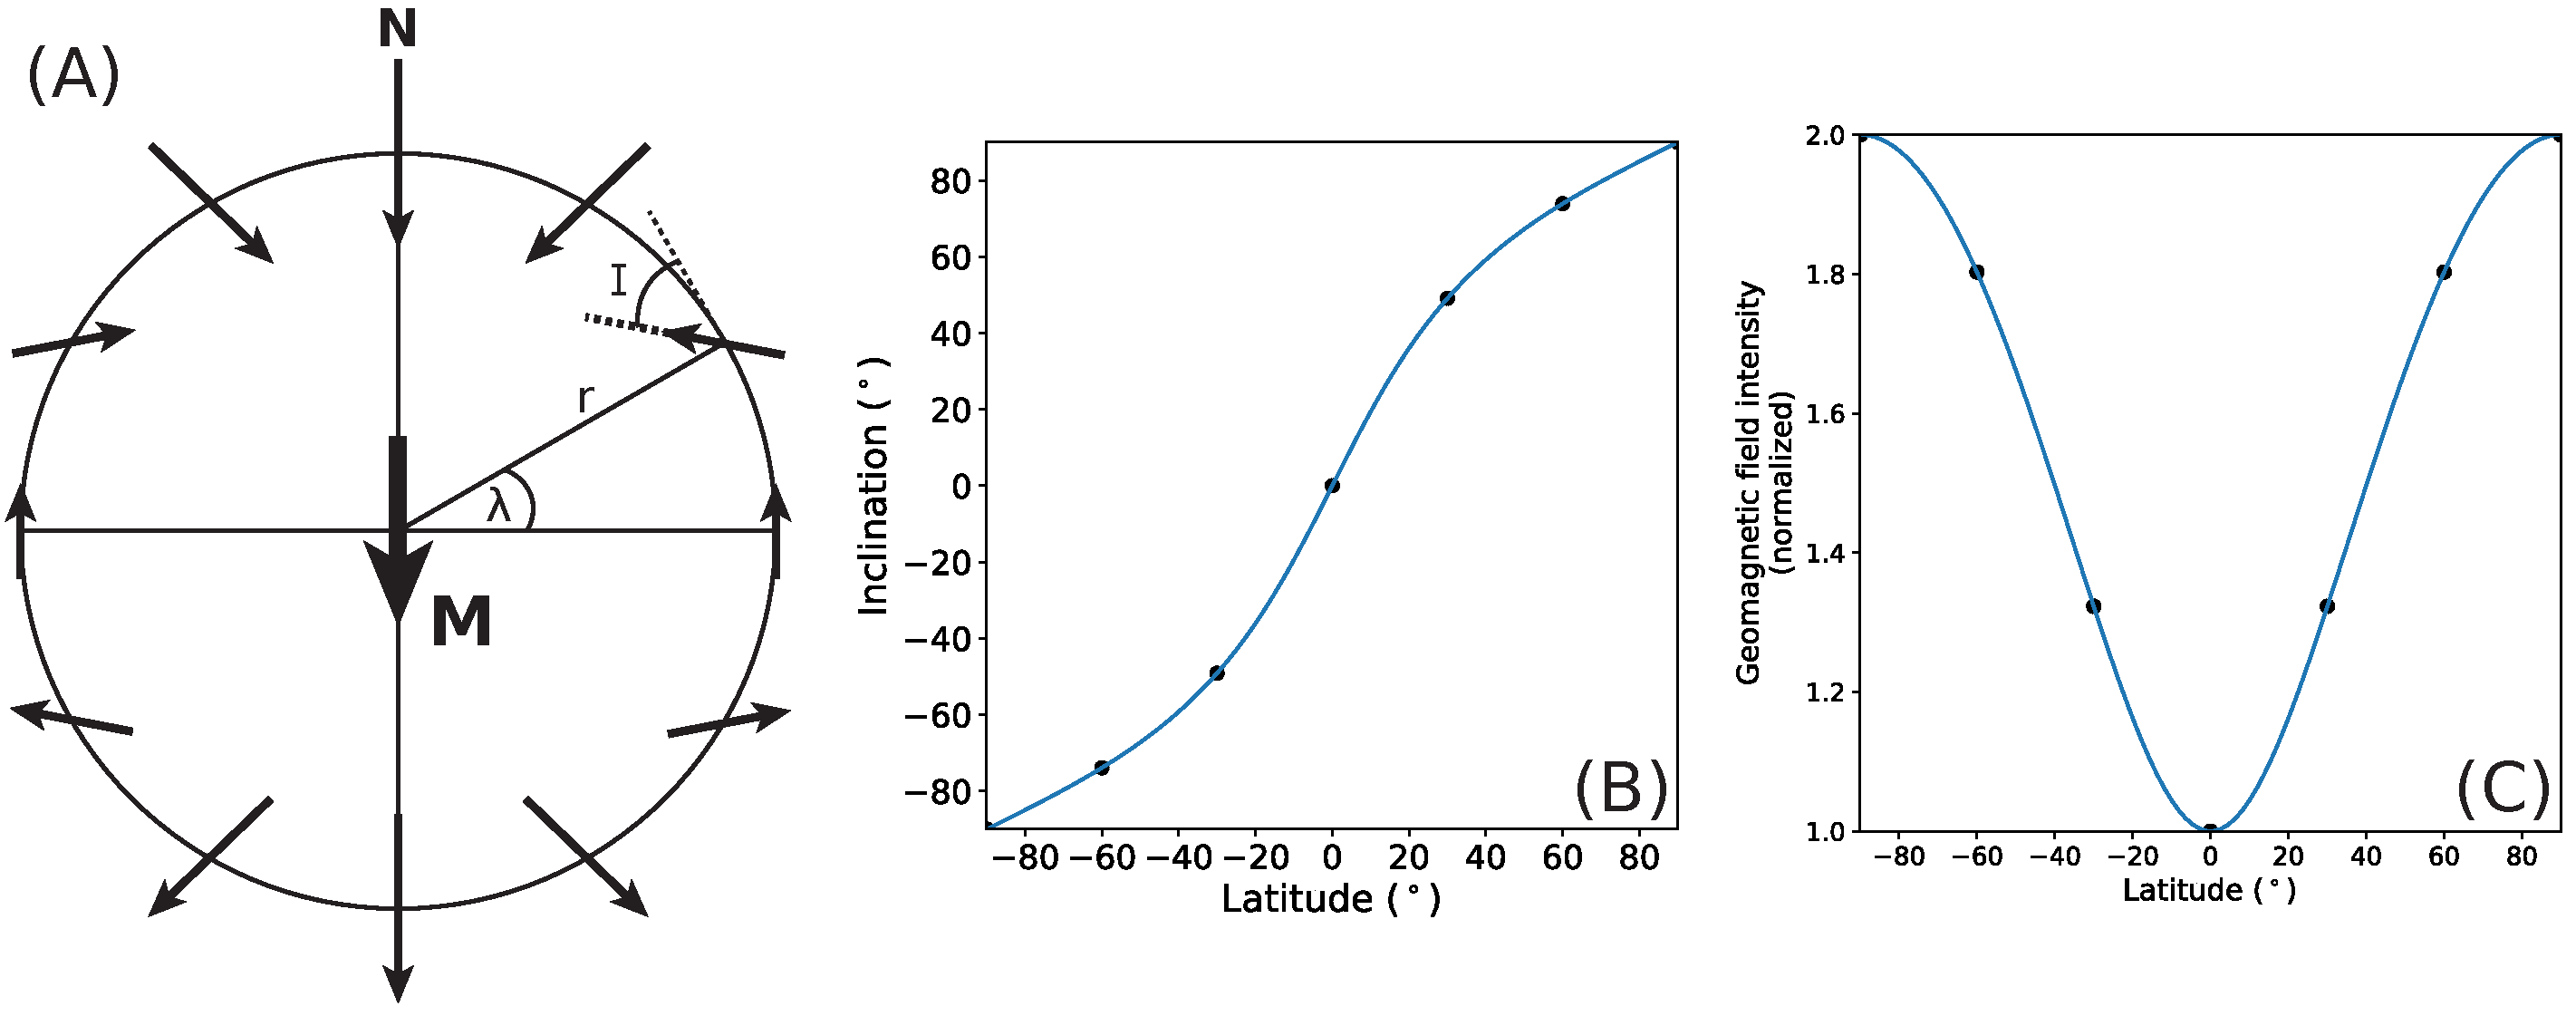
\includegraphics[width=\textwidth]{figure/GAD.pdf}
    \caption{(A) Geocentric axial dipole model. Magnetic dipole M is placed at the center of the Earth and aligned with the spin axis; the geographic latitude is $\lambda$; the mean Earth radius is $r$; the magnetic field directions and relative intensities at the Earth’s surface produced by the geocentric axial dipole are schematically shown by the arrows; inclination, $I$, is shown for one location; N is the north geographic pole. Modified after \cite{McElhinny1973a}. (B) Correlation between magnetic field inclination and latitude of a dipolar magnetic field. (C) Correlation between normalized magnetic field intensity and latitude of a dipolar magnetic field.}
    \label{fig:GAD}
\end{figure}

Effective ways of testing the robustness of the GAD hypothesis through time include comparing observed latitudinal dependence of paleomagnetic inclination data and intensity data with those predicted by the dipole equations. In addition, the symmetry of paleomagnetic reversals also provides insights into the dipolarity of the field, in that a geomagnetic field with a dominant non-dipolar component that does not reverse and a reversing dipolar component with minor contribution would have asymmetric reversals. It has been demonstrated that the GAD hypothesis is robust for the past 10,000 years on the basis of the magnetization of global compilations of archeological sites and sediments \cite[e.g.][]{McElhinny1996a}. For the past 5 million years, compilations of paleomagnetic data are best described with a GAD-dominated field with minor persistent contributions from non-dipole components (1-5 \%; \citep{Tauxe2005a, Valet2011b}). Statistical analyses of compilations of the relatively abundant paleomagnetic directional and intensity data further back in time show that Earth's magnetic field has been compatible with being GAD-dominated throughout the Phanerozoic \citep{Evans1976a, Lhuillier2023a}. The use of paleomagnetic data under the GAD assumption lies at the core of reconstructing past plate tectonic configurations \citep{Creer1954a, Irving1977a, Besse2002a, Torsvik2012a}. The GAD model gains support in the Phanerozoic in that the reconstructed plate motions are smooth with rates typically $<$20 cm/y \citep{Torsvik2012a}. Such results are independently verified by marine magnetic anomalies and hotspot tracks since the mid-Mesozoic \citep{Doubrovine2012a, Muller1993a}.

However, the Precambrian paleomagnetic observations challenge the uniformitariansm of a dipolar geomagnetic field through deeper time. There is increasing evidence that suggest Earth's magnetic field in the Ediacaran may not be GAD-dominated. Anomalously rapid changes in paleomagnetic field directions have been found in rocks from a variety of localities \cite[e.g.][]{Abrajevitch2010a, Meert2014a, Halls2015a}. Magnetostratigraphy data developed by \citep{Kodama2021a} show the Johnnie Formation records anomalously frequent reversals ($\sim$13 per Myr) in the Ediacaran. A series of low paleointensity values have been obtained primarily using single silicate crystals (i.e. dominantly monomineralic crystal aggregates) from Ediacaran rocks \citep{Bono2019a, Thallner2021a, Thallner2021b}. All these data have invoked a hypothesis that Earth's magnetic field was not GAD-dominated in the Ediacaran Period. Some studies have posited that these data indicate a time when the geodynamo reached its minimum prior to a recovery brought by the onset of inner core nucleation \cite[e.g.][]{Bono2019a}. Today, the characteristics of the geodynamo in the Ediacaran remain enigmatic, and the mechanism for the anomalous directional and intensity data remains debated \citep{Domeier2023a}.

In the Proterozoic, it had also been previously hypothesized that non-dipole components dominated the geomagnetic field. Prior to the high-precision geochronology data and detailed paleomagnetic data was developed within a volcanostratigraphic context became available, the apparent asymmetry in paleomagnetic field reversal records in Midcontinent Rift rocks led \citep{Halls1982a, Pesonen1981a} to interpret there being a significant non-GAD field component in the late Mesoproterozoic. However, high-resolution paleomagnetic data that span three geomagnetic field reversals in a more detailed stratigraphic context show each reversal was symmetric \citep{Swanson-Hysell2009a}. Since that work, more sophisticated statistical analyses have further clarified that the paleomagnetic pole progression recorded by rocks of the Midcontinent Rift represent rapid plate tectonic motions and does not require invoking a significant non-GAD geomagnetic field component or a significant true polar wander event \citep{Swanson-Hysell2019a, Rose2022a}. 

Additional statistical analyses by \citep{Tauxe2009a} show that the shape of the distribution of the paleomagnetic directional data recorded by lava flows of the North Shore Volcanic Group is consistent with that of the past 5 million years (model TK03 of \cite{Tauxe2004b}). My collaborative work with \citep{Pierce2022a} also show that correcting the inclination shallowing of syn-rift hematite-bearing sedimentary rocks of the Cut Face Creek Sandstone to be conformable with the field pattern of the TK03 model results in a mean direction that agrees with that recorded by the volcanic rocks that bracket the sedimentary rocks. These analyses support the interpretation that the geomagnetic field at Midcontinent Rift time was consistent with being dipole-dominated and had a secular variation patter similar to that of recent geologic times. The analyses of \citep{Gong2023a} show that paleomagnetic directional observations across Laurentia in the late Mesoproterozoic can be better fit with a dipole than a quadrupole configuration. Overall, the enriching paleomagnetic directional and intensity data in the Proterozoic have been adding increasing support for there being a GAD-dominated geomagnetic field through the Proterozoic Eon \citep{Veikkolainen2014a, Salminen2017a, Veikkolainen2021a, Gong2023a}. 

With confidence in the GAD-dominated field in the Mesoproterozoic, we can utilize paleomagnetic directional data to explore temporal associations between rock units when radiometric chronological constraints are not available. In chapter 1 I develop new paleomagnetic data from the ca. 1092 Ma Beaver River diabase and compare their pole position to that of the Greenstone Flow of the Portage Lake Volcanics. The agreement between the pole positions between the rift extrusive and intrusive rocks indicate close temporal linkage and leads way to a magmatic linkage between the two units. In chapter 3, I develop new paleomagnetic data from mafic intrusive and extrusive rocks in southwestern Laurentia and investigate the extent of the southwestern large igneous province, and its temporal and magmatic relationship with the Duluth Complex. These new data add to the existing paleomagnetic database for Laurentia for the reconstruction of the Keweenawan Track---the the late Mesoproterozoic apparent polar wander path of Laurentia which is central to the reconstruction of global paleogeography leading up to the assembly of the Rodinia supercontinent. 

\subsection{Using detrital remanent magnetization in hematite-bearing sedimentary rocks for paleogeographic reconstructions}

Sedimentary rocks are important archives of paleomagnetic records that provide major contributions to global paleogeography reconstructions \cite[e.g.][]{Torsvik2012a, Domeier2012a, Vaes2023a}. While igneous rocks acquire thermal remanent magnetizations during cooling through blocking temperatures of ferromagnetic minerals, sedimentary rocks acquire detrital remanence magnetizations as a result of preferential alignment of detrital ferromagnetic particles with local magnetic field during deposition. In the Midcontinent Rift, clastic sedimentary rocks of the Oronto Group deposited during post-rift thermal subsidence following the bulk of rift magmatic activity provide paleomagnetic poles that extend the Keweenawan Track to ca. 1070 Ma \citep{Henry1977a, Slotznick2023a}. 

However, the accuracy of paleomagnetic directions recorded by the detrital remanent magnetization of sedimentary rocks has long been recognized as problematic due to the issue of inclination shallowing \citep{King1955a, Kodama2012a, Tauxe1984a, Van-Andel1966a}. The rotation of ferromagnetic grains during deposition and compaction can result in the acquisition of a detrital remanence that is biased shallow relative to the local geomagnetic field in which it was acquired \citep{Tauxe2005a}. Mathematically, the effect of inclination shallowing can be described as 
\begin{equation*}
\textup{tan}(I_o) = f\textup{tan}(I_f)
\end{equation*}
where $I_o$ represents the observed inclination of the specimen magnetization and $I_f$ represents the inclination of the field in which the magnetization was acquired. If uncorrected, shallower inclinations obtained from sedimentary rocks can potentially result in erroneously low estimates of paleolatitudes, biasing the interpreted past positions of continents and hindering plate reconstructions.

Experimental methods such as magnetic fabric analyses \cite[e.g.][]{Kodama1995a, Bilardello2010a, Bilardello2010b, Bilardello2010c} as well as statistical approaches \cite[e.g.][]{Tauxe2004b} have been developed for correcting inclination shallowing in sedimentary records. However, there had been limited efforts in reporting uncertainties associated with the amount of shallowing, let alone propagating such uncertainties into paleogeographic reconstructions. I developed a new method of representing the uncertainties associated with inclination shallowing by using a spherical bivariate Kent distribution to represent uncertainty associated with paleomagnetic mean pole position through collaboration with an undergraduate honors thesis project at Berkeley Earth and Planetary Science which is published as \citep{Pierce2022a}. This method has had successful applications in paleogeography reconstructions \citep{Slotznick2023a, Vaes2023a, Zhang2024a}. 

% add inclination shallowing cartoon
\begin{figure}[h!]
    \centering
    \includegraphics[width=0.6\textwidth]{figure/inclination_shallowing.pdf}
    \caption{The relationship between the inclination of the local magnetic field compared to the observed inclination of sedimentary rocks is shown for different flattening factors (f). A value of 1.0 corresponds to no flattening while a value of 0.0 means the magnetizations are completely flattened. Figure modified after \cite{Pierce2022a}.}
    \label{fig:inclination_shallowing}
\end{figure}

In chapter 4, I develop new paleomagnetic data from hematite-bearing sedimentary rocks of the Jacobsville Formation which overlies unconformably on top of Midcontinent Rift. \citep{Hodgin2022a} developed geochronology data that constrain the timing of deposition of the Jacobsville Formation to be associated with compressional deformation of the Grenvillian orogenesis ca. 990 Ma. I use a Kent mean paleomagnetic pole position to represent the pole position and associated uncertainty recorded by the Jacobsville Formation. That pole is the first constraint from Laurentia's interior for the global paleogeography in the earliest Neoproterozoic. In that chapter I will show that the data together with the Keweenawan Track support the tectonic model where Laurentia traveled rapidly equatorward in the latest Mesoproterozoic and significantly slowed down following the onset of the Grenvillian orogenesis. 

\subsection{The global paleogeography in the earliest Neoproterozoic: progress and future directions}

The evolution of the configuration of ancient continents is foundational to our knowledge of global tectonics, geodynamics, and climate through Earth history. We know that in the late Proterozoic, ancient continents conjoined together to form the supercontinent Rodinia \citep{Swanson-Hysell2021c}. The position of Laurentia is particularly crucial given its central location in the supercontinent. Extensively studied paleomagnetic records of volcanics and intrusions associated with the Midcontinent Rift provide crucial constraints on the paleogeography of Laurentia in the late Mesoproterozoic Era \citep{Halls1982a, Swanson-Hysell2019a}. The apparent polar wander path of Laurentia, the Keweenawan Track, is a central record for reconstructing the assembly of the ancient supercontinent Rodinia \citep{Evans2021b}. The Keweenawan Track records rapid equatorward motion associated with the closure of the Unimos Ocean basin between Laurentia and conjugate continents leading up to the collisional Grenvillian orogeny that assembled Rodinia. The Grenvillian orogeny initiated ca. 1090 Ma with peak metamorphism of the Ottawan Stage of the orogeny occurring ca. 1050 Ma, but with protracted collisional orogenesis continuing through the 1020 to 980 Ma Rigolet Stage \citep{Rivers2008a, Rivers2012b, Swanson-Hysell2023a}. This later stage of the orogeny led to the formation of the Grenville Front as contractional deformation propagated further into the continent. 

\begin{figure}[h!]
    \centering
    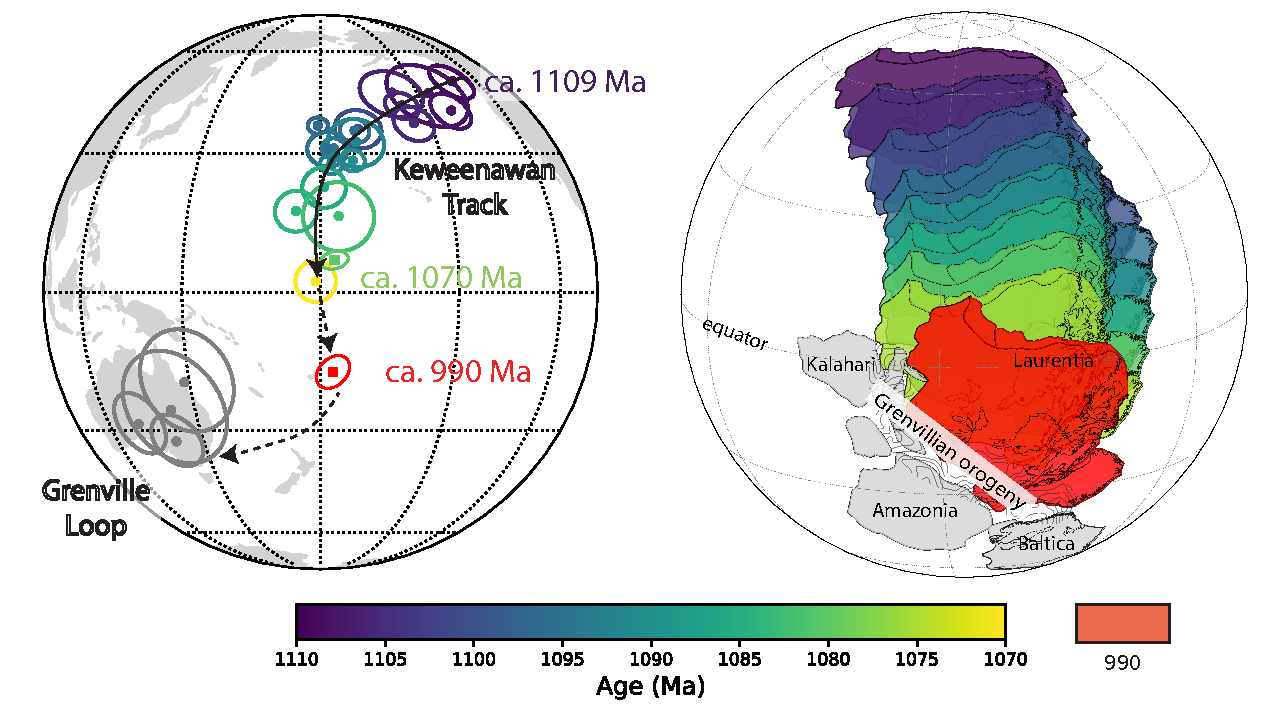
\includegraphics[width=\textwidth]{figure/pole_summary.pdf}
    \caption{Summary paleomagnetic data and paleogeography reconstruction for Laurentia through the late Mesoproterozoic to the early Neoproterozoic. Left panel shows a compilation of paleomagnetic poles that constructs the ca. 1109-1070 Ma Keweenawan Track, the ca. 990 Ma Jacobsville Formation pole, and the Grenville Loop poles. Right panel shows a snapshot of paleogeography reconstruction ca. 990 Ma. Positions of Laurentia and the conjugate continents along Laurentia's present-day eastern margin where Grenville orogenesis occurred are shown based on the Jacobsville pole and previously published paleomagnetic and geologic constraints. The details of the data compilation and reconstructions are presented in Chapter 3.}
    \label{fig:paleogeography}
\end{figure}

However, following the ca. 1084 Ma cessation of magmatism in the Midcontinent Rift and coeval volcanism in southwestern Laurentia \citep{Bright2014a, Mohr2024a}, there was a $\sim$300 Myr quiescence in known intracratonic magmatic activity in Laurentia that lasted until the emplacement of the ca. 775 Ma Gunbarrel large igneous province \citep{Harlan2003a, Mackinder2019a, Swanson-Hysell2021c}. Although the sedimentary records of the Oronto Group in the Midcontinent Rift basin help constrain the paleogeography of Laurentia at the latest Mesoproterozoic, the lack of well-dated paleomagnetic constraints from Laurentia's interior in the Neoproterozoic leaves the paleogeography of Rodinia poorly constrained between its initial assembly and breakup. 

Additional paleomagnetic constraints for Rodinia following the onset of the Grenvillian orogenesis have been obtained from the metamorphosed rocks of the orogen \cite[e.g.][]{Irving1972a, Berger1979a}. Metamorphic thermobarometry studies have found that regional metamorphism of the Grenville orogen reached up to Granulite facies with peak metamorphism temperatures estimated to be $\sim$750\textdegree C \citep{}, possibly even higher \citep{Shinevar2021a, Metzger2021a}. Such temperatures are above the Curie temperature of magnetite ($\sim$580\textdegree C) and the N\'eel temperature of hematite ($\sim$680\textdegree C). Therefore, rocks of the Grenville orogen would have had their remanent magnetization acquired during initial formation entirely erased by heating during peak metamorphism, and subsequently overwritten during cooling associated with exhumation long after peak metamorphic conditions \citep{McWilliams1975a}. Paleomagnetic poles from the Grenville orogen cluster in a position that is significantly south to the end of the Keweenawan Track, as well as the positions of later Neoproterozoic paleomagnetic poles. That Laurentia's apparent polar wander path loops down along the Keweenawan Track to the poles from the Grenville orogen and then back up again has led to them being referred to as the ``Grenville Loop'' \citep{Berger1979a}. Given that Laurentia had a central position within Rodinia, reconstructions of the supercontinent are heavily reliant on these pole positions and the ages that are assigned to them both in terms of the supercontinent's absolute position and the relative configuration between different cratons and Laurentia. 

Determining the age of the the timing of remanence acquisition in rocks of the Grenville orogen requires constraining the cooling history of the orogen. Pioneering work pairing thermochronology with paleomagnetic data recognized the long duration of cooling within the orogen and the necessity of determining cooling curves to assign ages to paleomagnetic poles \citep{Berger1979a}. This work has subsequently been built upon through the development of additional $^{40}$Ar/$^{39}$Ar and U-Pb thermochronology data (e.g. \citep{Mezger1991a, Warnock2000a}) and the use of cooling curves interpreted from such data to interpret ages of paleomagnetic poles (e.g. \citep{Warnock2000a, Brown2012a}). As a result, high latitude Grenville Loop poles from the Haliburton intrusions in Ontario and the Adirondack Highlands have been assigned ages of 1015 Ma, 990 Ma, and 970 Ma. Albeit that these age assignments to Grenville Loop poles are based on rough estimates of the timing of magnetic remanence acquisition along simplified interpolation of cooling history paths, they have been incorporated into curated paleomagnetic database for paleogeography reconstructions \cite[e.g.][]{Weil2003a, Evans2021a}. As is shown in Figure \ref{fig:pole_plot}, paleomagnetic poles of the Grenville Loop plot near Australia in present-day coordinates; forming arc distances of $\sim$50\textdegree\ from poles at the end of the ca. 1110 to 1070 Ma Keweenawan Track.

The now well-dated ca. 990 Ma paleomagnetic pole position of the Jacobsville Formation from Laurentia's interior in chapter 4 challenges the previous age assignments to the Grenville poles. In Figure \ref{fig:pole_plot}, the Grenville Loop poles also plot far away from the new Jacobsville pole. That ages assigned to the Grenville Loop are both the same and bracketing the age of the Jacobsville pole presents a conundrum given the very different positions they imply for Laurentia and associated continents in Rodinia (Fig. \ref{fig:paleogeography}). In chapter 4, robust field tests constrain the Jacobsville pole to be a primary detrital remanent magnetization that is chronostratigraphically well-constrained. We consider it to be a more reliable representation of the position of Laurentia ca. 990 Ma. However, there is a wealth of paleomagnetic data from the Grenville orogen that consistently reproduce the high-latitude pole position. Given that the Jacobsville pole is temporally associated with the last pulse of Grenvillian contractional deformation --- it was deposited in a synorogenic basin as the Grenville Front developed and propagated into the interior of Laurentia --- solutions for this discrepancy that call upon separation between Laurentia and the Grenville Province at the time are not feasible. The Grenville poles must be a representation of Laurentia's paleogeographic position, but the question is at what time? 

In previous Grenville paleomagnetic literature, the lack of reporting uncertainties associated with these age assignments is partly due to the lack of using quantitative methods to reconstruct probable thermal history paths based on the thermochronology data. The fact that measurement level data and specimen-specific details such as grain sizes are not available for the historic thermochronology literature makes it difficult to reproduce or improve those estimated ages. Additional uncertainty that was not fully taken into account in the previous literature comes from the cooling-rate dependence of magnetic remanence acquisition. In some contributions that have assigned ages to Grenville paleomagnetic poles, the Curie temperature of magnetite has been used as the temperature with which to assign an age to a magnetite magnetization from an interpreted cooling curve. While the Curie temperature is certainly relevant as above it the mineral is paramagnetic rather than ferromagnetic, blocking temperatures for an assemblage of grains will be below the Curie temperature. For populations of pre-existing magnetite, acquisition of magnetization occurs as a rock cools through temperatures where the thermal fluctuation energy is no longer sufficient to reset the magnetization of particles to align with the ambient field on a given timescale (the relaxation time). For rapidly cooled rocks such as lava flows, the cooling rate during emplacement and that during demagnetization in the lab are similar and the observed unblocking temperatures in the lab are close to the natural blocking temperatures during remanence acquisition (Fig. \ref{fig:slow_cooling}). In contrast to a rapidly cooled lava, magnetite-bearing rocks in the Grenville orogen acquired remanence during protracted cooling after peak metamorphism leading to a several orders of magnitude difference between the natural cooling rate and thermal demagnetization in the lab. This slow cooling leads to an expression of the cooling rate dependence where the temperatures at which a magnetization is acquired are lower than the temperatures at which it is removed in the lab (Fig. \ref{fig:slow_cooling}; \cite{Pullaiah1975b, Halgedahl1980a, Dodson1980a}). The example shown in Figure \ref{fig:slow_cooling}B compares the natural blocking temperature to the lab unblocking temperature for a cooling rate of 6\textdegree C/Myr using the framework of \citep{Dodson1980a}. In this case, magnetic remanence acquired at a temperature of 430\textdegree C would unblock in the lab at 500\textdegree C. Estimating the age of remanence acquisition in conjunction with cooling trajectories necessitates developing a framework that implements these relationships. These considerations further highlight how important it is to precisely determine the unblocking temperatures of magnetite-held remanence associated with a paleomagnetic direction. Previous efforts to assign ages based on cooling curves have typically picked single temperature values. 

I am interested in testing a hypothesis to explain the distinct pole positions between the Jacobsville pole and the Grenville Loop poles, which is that the poles from the Grenville orogen are younger than currently interpreted. Instead of the poles having remanence that was acquired while the Grenvillian orogeny was still ongoing (as is the case of the interpretation of the Haliburton pole; \citep{Warnock2000a}) or in the few 10s of millions of years following the Rigolet stage (as interpreted for the Adirondack poles; Fig. \ref{fig:thermal_history}), the magnetic remanence could instead have been acquired during exhumation well after the ca. 980 Ma cessation of contractional deformation. In this scenario, the migration of Rodinia to the higher latitude position represented by the Grenville Loop poles would have occurred further into the Neoproterozoic (Fig. \ref{fig:paleogeography}). Testing this hypothesis is of central importance to Neoproterozoic paleogeography as the ages associated with those Grenville Loop poles are crucial for constraining the motion of Laurentia at this time and the configuration between Laurentia and hypothesized conjugate continents. For example, in the case of Baltica it has been argued through comparison between paleomagnetic poles from the Grenville orogen and Sveconorwegian orogen that there were multiple oscillatory true polar wander rotations in the early Neoproterozoic \citep{Evans2015a, Gong2018a}. This interpretation is reliant on the assigned ages of the poles in both orogens. I plan to approach this question by developing high-precision U-Pb thermochronology data and new high-resolution paleomagnetic data. I will quantitatively construct thermal history paths and associated uncertainties using U-Pb apatite system as a thermochronometer which have closure temperatures similar to the blocking temperatures of titanomagnetite in Grenville rocks. I will pair these results with new high-resolution thermal demagnetization data such that the natural blocking temperature of the Grenville rocks can be better constrained based on the unblocking spectra obtained in the lab, taking the cooling-rate effect into consideration. 


\subsection{Probing the evolution of Earth's interior via paleointensity observations}

Earth's magnetic field is powered by convective flow of liquid iron-alloy in Earth's outer core. At present day, the geodynamo is collectively driven by heat flow across the core-mantle boundary and from the crystallization of the solid inner core from the liquid outer core which provides latent heat and compositional buoyancy due to the exclusion of light elements \citep{Buffett2000a}. The global entropy balance for the convective core that relates the Ohmic dissipation to thermal and compositional convection show that the the compositional energy is more efficient in maintaining the current energy dissipation \citep{Labrosse2003a, Landeau2022a}. A question thus arise regarding whether Earth has had an inner core since the beginning of its formation, and if not, when did the inner core begin to nucleate. Theoretical calculations show large uncertainties associated with the predicted timing of the inner core nucleation due to the lack of constraints on the thermal conductivity of the core \citep{Gubbins2004a, Konopkova2016a, Pozzo2012a, Ohta2016a}. Such uncertainties remain until further constraints on the core composition and agreements on experimental results of thermal conductivity values of iron-alloy become available in the literature. 

Paleomagnetic observations provide a unique tool that can provide constraints on the thermal evolution of Earth’s core. Based on paleomagnetic directional and intensity data, we know that an active dynamo  has existed since the 3.5 Ga \citep{Selkin2007a, Biggin2011a, Tarduno2014a, Brenner2020a, Brenner2022a} and probably earlier \citep{Tarduno2015a}. Theory and modeling predict that the nucleation of the inner core would produce a notable increase in the efficiency of convection in the outer core such that a notable increase in the surface geomagnetic field intensity may be observed and thus be reflected in the paleomagnetic intensity records \cite[e.g.][]{Labrosse2003a, Aubert2009a, Driscoll2016a, Landeau2022a}. 

Paleointensity experiments are used to reconstruct records of past geomagnetic field intensity from thermoremanent magnetizations based on the linear dependence of thermal remanence acquisition on the magnetic field present. Based on the single domain thermal remanence magnetization blocking theory of \citep{Neel1955a}, \citep{Butler1992a} deduced the following equation for the acquisition of thermal remanence magnetization (TRM) of a population of identical single-domain ferromagnetic grains when cooling in a constant magnetic field (H) from the blocking temperature ($T_B$) to ambient temperature ($T_0$):
\begin{equation}
    TRM [T_0] = N[T_B] v j_s [T_0] tanh(\frac{v j_s [T_B]H}{k T_B})
\label{PINT_eq_1}
\end{equation}
where $[T_0], [T_B]$ denote the temperature of the temperature-dependent parameters, $N[T_B]$ represents the number of single-domain grains per unit volume with blocking temperature $T_B$, $v$ is the volume of the single domain grains and $j_s$ is the saturation magnetization, k is the Boltzmann constant. This equation assumes the grains block in the remanence magnetization sharply when cooling through the blocking temperature $T_B$. Typically the term $\frac{v j_s [T_B]H}{k T_B}$ which measures the degree of alignment of the grains at the blocking temperature has a value $<<1$. Therefore, equation \ref{PINT_eq_1} becomes 
\begin{equation}
    TRM [T_0] = AH
\label{PINT_eq_2}
\end{equation}

where A is a generalized proportionality constant. A rock sample that acquires a thermal remanent magnetization that follows this linear relationship with the magnetic field that it cools in would thus have a proportionality constant $A$ which depicts both $TRM_{paleo}=AH_{paleo}$ and $TRM_{lab}=AH_{lab}$. Therefore, the paleointensity can be obtained by eliminating the proportionality constant, A, and 
\begin{equation}
    H_{paleo} = \frac{TRM_{paleo}}{TRM_{lab}}
\label{PINT_eq_3}
\end{equation}

% add paleointensity example plot
\begin{figure}[h!]
    \centering
    \includegraphics[width=0.6\textwidth]{figure/IZZI_protocol.pdf}
    \caption{Schematic Thellier paleointensity diagram showing an ideal experimental results using the ``in field-zero field-zero field-in field" paleointensity protocol developed by \citet{Yu2004a}.}
    \label{fig:IZZI_protocol}
\end{figure}

With this theoretical basis, \citep{Thellier1959a} developed the experimental protocol later known as the Thellier double-heating paleointensity method that features step-wise removal of the natural thermal remanence magnetization ($TRM_{paleo}$) and imposition of new partial thermal remanence ($TRM_{lab}$) in a known lab field through heating and cooling. This technique is based upon Thellier’s laws, which state that partial thermal remanence (pTRM) must be additive, independent (partial remanence acquired between distinct temperature steps is distinct from one another) and reciprocal (the unblocking temperature is the same as the blocking temperature. The resultant comparison between a sample's capability of acquiring a TRM in the lab and its acquired TRM in nature is then illustrated in the paleointensity plot first introduced by \citep{Arai1963a} (Figure). In an ideal experiment with ideal magnetic recorders, the relationship between natural remanence lost and pTRM gained is linear, and the slope of the best-fit line to the data is proportional to the intensity of the ancient field. Using this slope, and multiplying by the known lab field, one can calculate the ancient magnetic field strength. The Thellier method has subsequently been improved such that sample behaviors that diverge from being ideal single-domain described in the theory can be better detected \cite[e.g.][]{Coe1967b, Riisager2001a, Yu2003a, Yu2004a, Yu2006a}. Today, the ``in field-zero field-zero field-in field" (IZZI) Thellier paleointensity protocol combined with result filtering based on a series of statistical selection criteria is one of the most robust and widely used heating-based methods \citep{Yu2004a}. 

With the GAD assumption, Earth's (virtual) axial dipole moment can be calculated given known paleointensity and paleolatitude of a locality at a time (equation \ref{PINT_eq_1}, \ref{PINT_eq_2}). There are compilations of paleointensity data that show Earth's (virtual) axial dipole moment through history (Figure xxx; \citep[e.g.][]{Veikkolainen2014b, Bono2022b}). Based on a selected compilation, \citep{Bono2019a} interpreted that the existing Precambrian paleointensity database shows a monotonic decay of the geomagnetic dipole moment throughout the Proterozoic. Together with their new data developed from silicate crystals of the ca. 565 Ma Sept-$\hat{I}$les mafic intrusions with the Thellier–Coe paleointensity method which were interpreted to show near-zero values, \citep{Bono2019a} hypothesized that a geodynamo primarily driven by waning thermal convection might have persistent through the Proterozoic until the nucleation of the inner core, which they interpreted to have happened in the Ediacaran. \citep{Bono2019a} further argued that their results are consistent with modeling results using an approach combining dynamo simulations and theoretical scaling relationships that predicted that progressive decay of the field’s dipole moment would be followed by a rapid increase in geomagnetic field intensity soon after the onset of inner core nucleation such that a minimum in dipole moment would occur just before inner core nucleation \citep{Driscoll2016a}. 

% add VADM compilation plot highlighting the recent addition of data (say since 2019?) 
%\begin{figure}[h!]
%    \centering
%    \includegraphics{}
%    \caption{Caption}
%    \label{fig:VADM_compilation}
%\end{figure}

However, the geodynamo evolution model put forward by \citep{Bono2019a} was based on a sparse Precambrian paleointensity database and is challenged by more recent observations. Low paleointensity values similar to those in the Ediacaran have been observed in the Mesoproterozoic \citep{Lloyd2021b, Shcherbakova2022a, Shcherbakova2023a}, the Neoproterozoic \citep{Lloyd2021a}, the early-Cambrian \citep{Lloyd2022a}, and the Paleozoic \citep{Shcherbakova2021a}. These new data challenge the uniqueness of the Ediacaran weak geodynamo. In chapter 2, I develop new paleointensity data from the ca. 1092 Ma anorthosite xenoliths of the Beaver River diabase. The paleomagnetic directional data I developed in chapter 1 establish that the anorthosite xenoliths are stable remanence recorders that acquired remanence during cooling in the host diabase. I then used the ``IZZI" Thellier paleointensity protocol \citep{Yu2004a} to develop absolute paleointensity data from the same xenoliths and calculated the axial dipole moment of Earth's magnetic field. My data together with previous observations from rocks of the Midcontinent Rift show high paleointensity values ca. 1.1 Ga. Some of the xenoliths unequivocally show exceptionally high paleointensity values. Those high values require there being a strong dynamo in the late Mesoproterozoic, which does not fit in the interpreted Proterozoic monotonic decay trend hypothesized by \citep{Bono2019a}. 

Overall, the high paleointensity values of the Beaver River anorthosite xenoliths necessitate a strong late Mesoproterozoic geodynamo. The enriching paleomagnetic database for the Precambrian is revealing a more complex history if Earth's core than previously thought. The observational data from paleomagnetism are now stirring renewed interests in better understanding the core's material properties in deep-Earth conditions and in understanding the dynamic connections between the mantle and the core. 

\subsection{Recovering deep-time paleointensity records from silicate-hosted Fe-oxides}

Successful recovery of deep-time paleomagnetic records is dependent on rocks maintaining primary magnetic remanence. Rocks are assemblages of fine-grained ferromagnetic particles with various stability that are dispersed within a matrix of diamagnetic and paramagnetic minerals. Not all ferromagnetic particles can maintain a magnetic memory through deep time. The characteristic time through which a ferromagnetic grain is capable of maintaining a magnetization before spontaneous relaxation is a function of temperature, external magnetic field, composition, size, and shape. Theoretical derivations show that the most stable remanence carriers are single-domain particles with a narrow size range \citep{Butler1975a, Butler1992a}. For example, ensembles of magnetite grains with sizes ranging from a few tens of nanometers to up to one micron, and hematite grains with sizes up to 15 $\mu$m can maintain a stable magnetization for billions of years. Recent advances in micromagnetic modeling and fine-scale magnetic imaging show that stable ferromagnetic particles in geologic samples are likely to be more often in the single vortex state which behaves similarly to the single domain state \citep{Nagy2017a, Tauxe2020a, CortesOrtuno2022a}. 

Other ferromagnetic particles in rocks include multidomain grains (i.e. particles with multiple magnetic domains) and complex vortex states (or pseudo-single-domain grains) which have more complex magnetic behaviors \citep{Williams2010a}. While some of them may be capable of maintaining primary paleomagnetic directional records through deep time, others are more prone to having their magnetizations be overwritten by heating or prolonged immersion in Earth's magnetic field postdating the acquisition of the primary remanence. Results of such processes typically manifest in rock samples as superposition of secondary remanence components on top of variably preserved primary remanence. 

While isolation of primary paleomagnetic directional data from secondary overprints is possible via step-wise thermal demagnetization experiments and vector subtractions, the existence of multidomain and complex vortex state grains complicate the determination of paleointensity records as their remanence acquisition and removal behaviors deviate from the Thellier laws. In addition, alteration of rocks in nature and in the lab can also complicate paleomagnetic records by changing the magnetic mineralogy. This could result in the destruction of original minerals and the formation of new magnetic minerals associated with chemical alteration during heating in the lab. Such mineralogical alterations are detrimental to paleointensity experiments, since the acquired remanence during the in-field steps in the lab would be held by grains distinct from those that record the natural remanence. Due to such complexities, recovering deep time paleointensity records is usually more difficult than paleomagnetic directional records. 

It has been found that ferromagnetic grains enshrouded by silicate mineral hosts can be well-protected from alteration and be faithful paleointensity recorders \citep{Cottrell1999a, Cottrell2000a, Tarduno2005a, Tarduno2005a, Tarduno2006a, Cottrell2008a, Selkin2000a, Selkin2007a, Selkin2008a}. In particular, titanomagnetite grains hosted in plagioclase crystals are intriguing targets. Petrography, electron microscopy, and microprobe data have shown that minor amount ($<$1\% by weight) of iron commonly exist in plagioclase crystals which can be present as fine-scale magnetite needles \citep{Selkin2000a, Feinberg2005a, Feinberg2006a, Wenk2011a, Bian2021a}. Rock magnetic analyses show that many of the rocks have ferromagnetic mineral assemblages dominated by single-domian-like behaviors with stable remanence carrying abilities. In addition, the alteration of the plagioclase does not readily result in the formation of secondary iron oxides in contrast with Fe-silicate minerals such as olivine and pyroxene. 

In chapter 2, I develop new paleointensity data using the anorthosite xenoliths of the Beaver River diabase in the Midcontinent Rift to characterize Earth's magnetic field ca. 1092 Ma. Electron microscopy images show that plagioclase crystals within these anorthosite xenoliths can enclose small pyroxene crystals which have fine-scale exsolved titanomagnetite grains. These observations corresponds to rock magnetic data that a number of the xenoliths typically have a dominant population of stable single-domain-like particles. The failed intracontinental rift nature of the Midcontinent Rift results in the anorthosite xenoliths being distant from subsequent tectonic events along Laurentian margins such that the lithology and magnetization of the anorthosite xenoliths have been minimally altered following initial formation. 

% replot Butler 1975 a single domain diagram
%\begin{figure}
%    \centering
%    \includegraphics{}
%    \caption{Caption}
%    \label{fig:Butler_single_domain}
%\end{figure}


% show example vortex-state grain and stability field 
%\begin{figure}
%    \centering
%    \includegraphics{}
%    \caption{Caption}
%    \label{fig:micromagnetic_model}
%\end{figure}

%\bibliography{YZ_ref}

\end{abstract}


\begin{frontmatter}

\tableofcontents
\clearpage
\listoffigures
\clearpage
\listoftables

\clearpage

\chapter*{Preface}
\phantomsection % make the ToC links work
\addcontentsline{toc}{chapter}{Preface} % add to ToC

The material within the chapters of this dissertation are largely taken from previously published (or soon to be published) articles. The following text identifies these articles, and provides brief summaries of each chapter.

\subsection{Chapter 1 - Synchronous emplacement of the anorthosite xenolith-bearing Beaver River diabase and one of the largest lava flows on Earth}

Zhang, Y., Swanson-Hysell, N.L., Schmitz, M.D., Miller Jr., J.D., and Avery, M.S., (2021), Synchronous emplacement of the anorthosite xenolith-bearing Beaver River diabase and one of the largest lava flows on Earth. Geochemistry, Geophysics, Geosystems. doi: \url{10.1029/2021GC009909}
\\

While magmatic activity within the 1.1 Ga North American Midcontinent Rift was protracted, it was punctuated by rapid pulses of voluminous magmatic activities. One of these pulses is represented in the massive \textit{ca.} 1096 Ma Duluth Complex while another is the \textit{ca.} 1092 Ma Beaver Bay Complex. A remarkable aspect of the Midcontinent Rift compared to most large igneous provinces is the extensive exposure both of extrusive lava flows and intrusive suites. Typically in a large igneous province one sees either the continental flood basalts (with the intrusions still in the subsurface) or the intrusions (with the extrusive flows having been eroded away). The exposure of both intrusive and extrusive units provides opportunities to more fully characterize the magmatic system and establish linkages. In this study, I developed paleomagnetic directional data from the anorthosite and the diabase, and collaborated with Professor Mark Schmitz and Professor Jim Miller to use paleomagnetic data, geochronology data, and geochemistry data to establish such an intrusive-extrusive connection. We show evidence that the anorthosite-bearing Beaver River diabase outcropping in northeastern Minnesota acted as a feeder system for the Greenstone Flow --- one of the largest single mafic lava flows on Earth.

The Beaver River diabase contains abundant anorthosite xenoliths liberated from a lower crustal cumulate. These xenoliths can exceed 150 meters which illuminates the large magma transfer enabled by wide conduits as magma transited to the near-surface and erupted into the rift basin. Thermal history modeling, U-Pb geochronology and paleomagnetic data from these anorthosite xenoliths illuminates their origin and history. Overall, we highlight that the rapid emplacement of the intrusive Beaver River diabase, anorthosite xenoliths therein, and the extrusive Greenstone Flow together punctuate a rapid and voluminous magmatic activity \textit{ca.} 1092 Ma during the Midcontinent Rift. 

Data and code used in this article are available on GitHub at \url{https://github.com/Swanson-Hysell-Group/2021_AX_BD} and on Zenodo at \url{https://zenodo.org/records/5394529}. 

\clearpage 

\subsection{Chapter 2 - High geomagnetic field intensity recorded by anorthosite xenoliths requires a strongly powered late Mesoproterozoic geodynamo}

Zhang, Y., Swanson-Hysell, N.L., Avery, M.S., Fu, R.R., (2022), High geomagnetic field intensity recorded by anorthosite xenoliths requires a strongly powered late Mesoproterozoic geodynamo. PNAS. doi: 10.1073/pnas.2202875119
\\

Acquiring high-fidelity observational records of ancient magnetic field intensity from the remanent magnetization of rocks is crucial for constraining the long-term evolution of Earth’s core. However, robust estimates of ancient field strengths are often difficult to recover due to alteration or non-ideal rock magnetic behavior. In this contribution, I developed high-quality paleointensity data with the best site-level standard deviation of 0.04 $\mu$T from well-preserved anorthosite xenoliths of the Beaver River diabase which were rapidly emplaced during the ca. 1.1 Ga North America Midcontinent Rift. The primary interpretation for the high paleointensity values gains strong support for there being a strongly powered geodynamo during the late Mesoproterozoic. These observations agree with previous results from Midcontinent Rift volcanic rocks and support such a strong field could have lasted at least 14 Myr. Together, paleointensity records from the Midcontinent Rift are inconsistent with there being a progressive monotonic decay of Earth’s dynamo strength through the Proterozoic Eon.
Our updated paleointensity data compilation show multiple observed paleointensity transitions from weak to strong in the Phanerozoic and the Proterozoic. Given that these records cannot all be the minimum prior to the beginning of inner core nucleation, they instead could indicate that processes such as plate tectonics could have modulated the core-mantle heat flow pattern in the Proterozoic. Regardless of when the initiation of inner core nucleation occurred, the observation of large variability in paleointensity in the Precambrian may present challenges in detecting the increase in surface geomagnetic field strength predicted by numerical models to have happened at the onset of inner core crystallization.

Data and code used in this article are available on GitHub at \url{https://github.com/Swanson-Hysell-Group/AX_BD_PINT} and on Zenodo at \url{https://doi.org/10.5281/zenodo.6658064}.
 
\clearpage 

\subsection{Chapter 3 - Paleomagnetism of the southwest Laurentia large igneous province and Cardenas Basalt: pulsed magmatism during rapid late Mesoproterozoic plate motion}

Mohr, M.T., Schmitz, M.D., Swanson-Hysell, N.L., Karlstrom, K.E., Macdonald, F.A., Holland, M.E., Zhang, Y., Anderson, N. (2024). High-Precision U-Pb geochronology links magmatism in the SW Laurentia Large Igneous Province and Midcontinent Rift. Geology. 
\\
\noindent Zhang, Y., Anderson, N., Mohr, M.T., Schmitz, M.D., Macdonald, F.A., Nelson, L.L., Thurston, O.G. Guenthner, W.R., Karlstrom, K.E., Swanson-Hysell, N.L. (2024). Widespread mafic magmatism across Laurentia in the late Mesoproterozoic: new paleomagnetic data from southwestern Laurentia. Submitted to JGR: Solid Earth. 
\\

High-precision geochronology data show that the emplacement of the ca. 1096 Ma voluminous mafic Duluth Complex and associated $\sim$ 8 km thick lava flows of the North Shore Volcanic Group occurred within 500 Kyr---consistent with these units being a large igneous province. In \cite{Mohr2024a} we show more high-precision geochronology data from the southwestern Laurentia that there was a ca. 1098 Ma pulse of large-igneous-province style mafic magmatism featuring the emplacement of thick mafic sills across at least eastern California and central Arizona. Geochronology data from that work further show that the Cardenas Basalt lava flows which were thought to be surface expressions of the ca. 1098 Ma mafic sills, are actually ca. 1082 Ma in age, indicating that they occurred during a distinct magmatic episode in the Grand Canyon. In this study, I develop new paleomagnetic data from mafic sills in Death Valley with Nick Anderson, and I developed new paleomagnetic data from mafic intrusions and the Cardenas Basalt in the Grand Canyon. These new data help better delineate the extent of the ca. 1098 Ma southwestern Laurentia large igneous province.

Prior to this work, late Mesoproterozoic global paleogeography reconstruction largely depends on the high-quality dataset from the Midcontinent Rift. New paleomagnetic data from this study provides independent support for there being a large latitudinal change in Laurentia's paleogeographic position at the time due to rapid plate tectonic motion. The new paleomagnetic pole from the Cardenas Basalt help further improve Laurentia's apparent polar wander path in the late Mesoproterozoic.

Data and code used in this study are available on GitHub at \url{https://github.com/Swanson-Hysell-Group/Cardenas_Unkar} and on Zenodo at \url{https://doi.org/10.5281/zenodo.}.

\clearpage 

\subsection{Chapter 4 - Tracking Rodinia into the Neoproterozoic: new paleomagnetic constraints from the Jacobsville Formation	Tracking Rodinia into the Neoproterozoic: new paleomagnetic constraints from the Jacobsville Formation}

Zhang, Y., Hodgin, E.B., Mohr, M.T., Alemu, T.B., Pierce, J., Fuentes, A.J., Swanson-Hysell, N.L. (2024). Tracking Rodinia into the Neoproterozoic: new paleomagnetic constraints from the Jacobsville Formation. Tectonics. 
\\

The assembly of the supercontinent Rodinia in the late Proterozoic is a pivotal event in the history of global tectonics. However, there has been a lack of well-dated paleomagnetic poles for its central piece, cratonic North America, for 300 Myr between the onset of the assembly ca. 1070 Ma and the initial break up of the supercontinent ca. 770 Ma. In this study, I developed high-quality paleomagnetic data from the Jacobsville Formation paired with previously developed state-of-the-art geochronology results to constrain cratonic North America's paleogeographic position ca. 990 Ma. The primary interpretation for this pole gains support from both an intraformational conglomerate test and a fold test. 
 
Our new high-quality paleomagnetic pole shows Laurentia's plate motion to have slowed down significantly following a previous period of rapid plate tectonic motion in the late Mesoproterozoic. Such slowdown in plate motion is coincident with the Grenvillian orogenesis along Laurentia's margin. This aspect of the results is quite interesting in terms of the tectonics and ties in with the geodynamics of the orogeny and supercontinent assembly. Our new pole adds a reliable constraint in the early Neoproterozoic that will be at the heart of future efforts to reconstruct the paleogeography of Rodinia.

Data and code used in this study are available on GitHub at \url{https://github.com/Swanson-Hysell-Group/Jacobsville} and on Zenodo at \url{https://doi.org/10.5281/zenodo.}.

\begin{acknowledgements}
\phantomsection % make the ToC links work
\addcontentsline{toc}{chapter}{Acknowledgements} % add to ToC
I thank my Ph.D. advisor, Nicholas Swanson-Hysell for bringing me to Berkeley. I always look up to him as a role model in scientific research and in life. His adept field geology skills, broad scientific interests and rigorous science ethics constantly challenged me to be a better scholar. I thank Nick for providing many field work opportunities in different places. I especially appreciated that Nick kept his office door open and allowed numerous walk-in discussions. I am also grateful for the company in the past five years from Nick's family. I have always enjoyed my time in the field together with Sarah, Maddy, and Wilma. 

I thank Scott Bogue and Margi Rusmore, my research advisors at Occidental College for their encouragement and support for pursuing a doctoral degree. I treasure our meetings at Santa Cruz and Los Angeles in the past five years. I thank my qualification exam committee, including Ben Gilbert, Harriet Lau, and Fernando Perez. I thank Bruce Buffett and Fernando Perez for being on my thesis committee and helping me improve this dissertation. 

I thank my advisors for the courses where I taught as a graduate student instructor. I learned a lot about Berkeley local bedrock geology by teaching EPS 101 field geology and digital mapping with Nick Swanson-Hysell and Matt Gleeson. The special 2020 COVID edition of video shooting the field geology class will be a life-long memory. I thank Daniel Stolper for the EPS 50 course in Spring 2021. Engaging with undergraduate student through EPS 50 lab sessions helped me stay positive and enthusiastic while the world was at a lock down. 

I thank John Grimsich for providing me with hands-on experiences on the many excellent instruments hosted at Berkeley EPS. I am grateful for the many hours that John spent teaching me to make professional petrographic thin sections, tuning and using scanning electron microscopes, and using X-ray diffraction machine. I very much appreciate John's curiosity over wide topics and enjoyed our daily interactions working together. 

I especially thank my parents for supporting my study abroad in the past eight years. It is a privilege to be able to experience the oriental and occidental lives, and to find my own definition through studying and traveling. 

I am grateful to the organizations whose funding enabled the research during my graduate course. The funding sources include:

\vspace{5mm}
$\bullet$ University of California, Berkeley
    \vspace{5mm}

    \hspace{\parindent} - Hearts to Humanity Eternal Programs
    \vspace{5mm}
    
    \hspace{\parindent} - Cheveron-Xenel Gateway Fellowship, Berkeley International House
    \vspace{5mm}
    
    \hspace{\parindent} - UC Berkeley student conference travel grant
\vspace{5mm}

$\bullet$ Institute for Rock magnetism
    \vspace{5mm}
    
    \hspace{\parindent} - US visiting student fellowship
    \vspace{5mm}
    
$\bullet$ Institute on Lake Superior Geology
    \vspace{5mm}
    
    \hspace{\parindent} - ILSG Student Research Fund
    \vspace{5mm}
    
$\bullet$ Geological Society of America
    \vspace{5mm}
    
    \hspace{\parindent} - 2022 GSA Graduate Student Research Grant 
    \vspace{5mm}
    
    \hspace{\parindent} - 2023 AGeS3-Grad Geochronology Award
    \vspace{5mm}
    
$\bullet$ National Science Foundation
    \vspace{5mm}

    \hspace{\parindent} - Grant career award  (awarded to Nick Swanson-Hysell)
    \vspace{5mm}
    
    \hspace{\parindent} - Grant FRES  (awarded to Nick Swanson-Hysell)
    \vspace{5mm}
    
    \hspace{\parindent} - Grant MagIC  (awarded to Nick Swanson-Hysell)
    \vspace{15mm}
    
Last but not least, I thank the earth, for being such a beautiful cosmic palimpsest. 

\end{acknowledgements}

\end{frontmatter}

\pagestyle{headings}


%%%%%%%%%%%%%%%%%%%%
%%%%% CHAPTERS %%%%%
%%%%%%%%%%%%%%%%%%%%

\include{Chap_BBC}
\include{Chap_PINT}
\include{Chap_Jacobsville}
\chapter[Paleomagnetism of the southwestern Laurentia large igneous province and Cardenas Basalt: pulsed magmatism during rapid late Mesoproterozoic plate motion][southwestern Laurentia large igneous province]{Paleomagnetism of the southwestern Laurentia large igneous province and Cardenas Basalt: pulsed magmatism during rapid late Mesoproterozoic plate motion}

\let\thefootnote\relax\footnote{Zhang, Y., Anderson, N., Mohr, M.T., Schmitz, M.D., Macdonald, F.A., Nelson, L.L., Thurston, O.G. Guenthner, W.R., Karlstrom, K.E., Swanson-Hysell, N.L. (2024). Paleomagnetism of the southwestern Laurentia large igneous province and Cardenas Basalt: pulsed magmatism during rapid late Mesoproterozoic plate motion. Submitted to JGR: Solid Earth.}

\section{Abstract}

Mafic intrusions, lava flows, and felsic plutons in southwestern Laurentia have been hypothesized to be associated with the emplacement of a late Mesoproterozoic large igneous province. Improved geochronologic data resolve distinct episodes of mafic magmatism in the region. The ca. 1098 main pulse of southwestern Laurentia large igneous province (SWLLIP) magmatism is recorded by mafic intrusions across eastern California to central Arizona. A younger episode of volcanism resulted in eruptions that formed the ca. 1082 Ma Cardenas Basalt---the uppermost unit of the Unkar Group in the Grand Canyon. Using the interpretation that the mafic intrusions within the Unkar Group were feeders to the lavas, a paleomagnetic pole was developed by combining data from the intrusions and the lavas. With the updated geochronological constraints, we develop new paleomagnetic data from mafic sills in the SWLLIP. Overlapping poles between the Death Valley sills and rocks of similar age in the Midcontinent Rift is inconsistent with large-scale Cenozoic vertical axis rotations in Death Valley. We also develop a new paleomagnetic pole from the ca. 1082 Ma Cardenas Basalt (pole longitude=183.9\textdegree E, pole latitude=15.9\textdegree N, A$_{95}$=7.4\textdegree, N=18). The new paleomagnetic data are consistent with the pole path developed from time-equivalent rocks of the Midcontinent Rift, supporting interpretations that changing pole positions are the result of rapid equatorward motion. These data add to the record of Laurentia's rapid motion from ca. 1110 to 1080 Ma that culminated in collisional Grenvillian orogenesis and the assembly of Rodinia. 

\section{Introduction}

The ancient North American craton (Laurentia) has a rich record of Stenian (late Mesoproterozoic) mafic magmatism. In the Midcontinent Rift of the Lake Superior region, punctuated episodes of voluminous intrusions and associated volcanism have been dated between 1109-1084 Ma with high-precision geochronology (Figure \ref{fig:SWLLIP_overview}). Paleomagnetic data from these well-preserved and well-dated rift-related rocks within the Midcontinent Rift make up the majority of the Stenian database of paleomagnetic poles for Laurentia \citep{Evans2021a}. These data provide central constraints on global paleogeography during the assembly of supercontinent Rodinia \citep{Swanson-Hysell2021c, Evans2021b}. 

In southwestern Laurentia, widespread Stenian magmatism led to the emplacement of mafic intrusions and lava flows as well as felsic plutons (Figure \ref{fig:SWLLIP_overview}A; \citealp{Wrucke1966a, Shride1967a, Hendricks1972a, Howard1991a, Bright2014a}). Based on petrologic and geochemical data \cite[e.g.][]{Wrucke1966a, Wrucke1972a, Hammond1986a}, it was previously suggested that the mafic intrusions in the region were contemporaneous. However, in comparison to the Midcontinent Rift where extensive high-precision zircon U-Pb geochronology data have been developed (typically with analytical uncertainties $<$1 Myr; \citealp[e.g.][]{Swanson-Hysell2019a}), most ages from rocks associated with the Stenian southwestern Laurentia magmatism have been relatively imprecise (e.g. as compiled and developed in \cite{Bright2014a}). The broadly overlapping ages, albeit with large uncertainties, of rocks that outcrop in California, Arizona, New Mexico, and Mexico led \cite{Bright2014a} to hypothesize that they could be grouped as the southwestern Laurentia large igneous province (SWLLIP). \cite{Bright2014a} further suggested that a temporal overlap of magmatism in the SWLLIP and in the Midcontinent Rift was the result of a geodynamic linkage. However, the available geochronology data from the SWLLIP at the time was not precise enough to test this relationship with the distinct magmatic intervals within the Midcontinent Rift. 

\begin{figure}[h!]
\centering
\includegraphics[width=0.75\textwidth]{figure/Zhang2024b/overview.pdf}
\caption[Overview of the inferred extent of the southwestern Laurentia large igneous province and compilation of high-precision zircon U-Pb geochronology data]{(A) Map of North America showing the inferred extent of the southwestern Laurentia large igneous province (SWLLIP) modified from \cite{Bright2014a} in light brown color, a more strict version of the inferred extent of the SWLLIP based on encircling sills dated to be ca. 1098 Ma through the high-precision geochronology data of \cite{Mohr2024a} in dark brown, together with the Pikes Peak batholith \citep{Green1992b}, and the inferred extent of the Midcontinent Rift. The inferred trace of the Grenville Front is modified from \cite{Rivers2015a}. The inset boxes show the extent of maps in Figure \ref{fig:geologic_maps}. (B) Summary of high-precision zircon U-Pb geochronology data from southwestern Laurentia \citep{Mohr2024a} and from the Midcontinent Rift, highlighting the Duluth Complex and the associated North Shore Volcanic Group \citep{Swanson-Hysell2019a, Swanson-Hysell2021a}, the Michipicoten Island Formation \citep{Fairchild2017a}. The 1082.6 $\pm$ 0.3 Ma Colorado River Trough sill is located in the Dead Mountains in southeastern California. Each black bar represents a $^{206}$Pb/$^{238}$U zircon weighted mean age. The colored shaded regions associated with the black bars represent uncertainties of the mean ages at 95\% confidence level calculated with a Student's-T multiplier.}
\label{fig:SWLLIP_overview}
\end{figure}
    
Due to sparse geochronology data, temporal relationships between units in southwestern Laurentia are mostly inferred. In the Grand Canyon, it has been hypothesized that thick mafic sills and dikes that intrude Unkar Group sedimentary rocks are feeder systems for the Cardenas Basalt lava flows which are the uppermost unit of the Unkar Group \cite[e.g.][]{Hammond1990a, Timmons2005a}. This hypothesis is based on the spatial proximity and trace and major element concentration similarities of lava flows and nearby intrusions \citep{Larson1994a}. No direct field evidence exists for feeder relations. \cite{Hendricks1989a} considered the sills and flows to be from the same parent magma, but did discuss a possible interpretation that the more differentiated flows erupted later than the emplacement of the sills. Applying the assumption that the extrusive and intrusive rocks were coeval, \cite{Weil2003a} developed a paleomagnetic pole by grouping data derived from thirteen mafic intrusions and three Cardenas Basalt lava flows in the Grand Canyon. Similar directions had previously been developed for two Cardenas lava flows by \cite{Elston1973a}. \cite{Weil2003a} assigned an age of 1090.6 $\pm$ 4.5 Ma (2$\sigma$) to their pole based on an $^{40}$Ar-$^{39}$Ar age they developed from biotite interpreted to have formed within the host Unkar sedimentary rocks during the intrusion of a mafic sill. 

Paleomagnetic data have also been developed from SWLLIP mafic sills that intrude Apache Group sedimentary rocks in central Arizona \citep{Helsley1972a, Donadini2011a}. These studies interpreted sills with normal-polarity paleomagnetic directional data as coeval. \cite{Donadini2011a} developed a mean pole from some normal-polarity sills and considered the age of the pole to be that of a baddeleyite U-Pb age of 1088 $\pm$ 11 Ma (2$\sigma$; age from one sill later published by \cite{Bright2014a}). Although \cite{Harlan1993a} also obtained paleomagnetic samples of mafic sills in the same region with clearer distinction between individual cooling units, that the normal paleomagnetic pole of \cite{Donadini2011a} was reported with paired radiometric age assignment led it to be the pole that is included in recent curated paleogeographic compilations \cite[e.g.][]{Evans2021a}. Other sills in the region record reversed directions with steeper inclinations relative to the normal polarity directions \citep{Harlan1993a, Donadini2011a}. In the field guide of \cite{Donadini2012a}, an age of 1119 $\pm$ 10 Ma (weighted mean of $^{207}$Pb/$^{206}$Pb date of 2 baddeleyite grains) and a age of 1111.6 $\pm$ 8.9 Ma (concordia intercept age of a combination of baddeleyite and zircon dates) were reported for sills of reversed polarity---these geochronology data remain unpublished. Both the steep reversed directions and the geochronological data are consistent with these sills being emplaced during an interval of reversed polarity prior to or during ca. 1109 to 1105 Ma early-stage Midcontinent Rift magmatism \citep{Vervoort2007a, Swanson-Hysell2019a}.

More recently, \cite{Mohr2024a} developed chemical abrasion-isotope dilution-thermal ionization mass spectrometry (CA-ID-TIMS) high-precison U-Pb geochronology data from zircon separated from differentiated zones in thick mafic sills in southwestern Laurentia and from zircon separated by bulk dissolution methods (applying the approach of \cite{Oliveira2022a}) from a thick lava flow within the Cardenas Basalt (Figure \ref{fig:cardenas_strat}). Three sills in Death Valley were dated at 1097.91 $\pm$ 0.29 Ma, 1098.27 $\pm$ 0.27 Ma, and 1098.09 $\pm$ 0.91 Ma, two sills in western Grand Canyon at 1098.16 $\pm$ 0.59 and 1098.09 $\pm$ 0.34 Ma, and one sill in central Arizona at 1097.97 $\pm$ 0.12 Ma (all ages are presented with analytical uncertainties at 95\% confidence which is calculated including a Student’s-T multiplier; \cite{Mohr2024a}). These ages agree with each other within uncertainty (Figure \ref{fig:SWLLIP_overview}B) and suggest that the mafic intrusions across the region were rapidly emplaced in $\sim$0.25 Myr \citep{Mohr2024a}. The data indicate an episode of LIP-style mafic magmatism ca. 1098 Ma in southwestern Laurentia that postdates the early plateau stage of volcanism in the Midcontinent Rift and predates the emplacement of the ca. 1096 Ma Duluth Complex and thick main stage rift volcanics (Fig. \ref{fig:SWLLIP_overview}). The data are consistent with a model where a plume head arrived ca. 1098 Ma under southwestern Laurentia leading to generation of melt and the emplacement of thick mafic intrusions. This plume could have then spread along the base of the lithosphere toward the Midcontinent Rift where it facilitated the reinvigoration of magmatism associated with the emplacement of the Duluth Complex and the North Shore Volcanic Group \citep{Mohr2024a}. In addition, \cite{Mohr2024a} developed a new zircon U-Pb age of 1082.18 $\pm$ 1.25 Ma (95\% confidence) from a Cardenas Basalt lava flow. That age indicates that the eruption of the lavas postdated the widespread ca. 1098 Ma mafic intrusions by $\sim$16 Myr (Figure \ref{fig:SWLLIP_overview}B). Given the rapid apparent polar wander shown by the ca. 1109-1080 Ma Keweenawan Track \citep{Swanson-Hysell2019a}, the $\sim$16 Myr age difference between the Cardenas Basalt and thick mafic sills predict that they should record distinct paleomagnetic pole positions separated by a large angular distance. With the new chronological insights in hand, we develop new paleomagnetic data from the dated mafic sills and additional undated Mesoproterozoic intrusions in Death Valley and the Grand Canyon. We also develop new paleomagnetic data from lava flows of the Cardenas Basalt within the Grand Canyon with an increased number of sites as well as volcanostratigraphic context. 

\section*{Geological Background}
\subsection*{Mafic intrusions in the Crystal Spring Formation, Death Valley}

Rocks in the Death Valley region record the geological evolution of the southwestern margin of Laurentia since ca. 1.8 Ga in the Paleoproterozoic Era (\citealp{Tapani-Ramo1998a}; Figure \ref{fig:geologic_maps}A, \ref{fig:DV_GC_strat_columns}). The basement rocks include Paleoproterozoic para- and orthogneiss \citep{Wasserburg1959a, Barth2000a, Strickland2013a} and early Mesoproterozoic porphyritic quartz monzonite \citep{Labotka1980a}. The Pahrump Group is a 1.5 to 4 km thick mixed carbonate and siliciclastic succession that unconformably overlies these basement lithologies (Figure \ref{fig:DV_GC_strat_columns}; \citealp{Wright1974a, Macdonald2013a}. Formations of the Pahrump Group include the Mesoproterozoic Crystal Spring Formation, the Tonian Horse Thief Springs Formation, the Tonian Beck Spring Dolomite, and the Cryogenian Kingston Peak Formation \citep{Macdonald2013a, Mahon2014a}. A $>$300 Myr unconformity separates the Crystal Spring Formation, which contains mafic sills, and the overlying Horse Thief Springs Formation, which contains $<$775.4 $\pm$ 0.7 Ma detrital zircon (\citealp{Mahon2014a, Dehler2023a}; Figure \ref{fig:DV_GC_strat_columns}) and does not contain the sills. The region experienced Permian-Triassic contraction and magmatism \citep{Snow1991a, Stevens1997a} followed by the Mesozoic Cordilleran orogeny \citep{Burchfiel1992a, Burchfiel1970a, Snow1991a}. Neogene felsic and mafic magmatism (Figure \ref{fig:geologic_maps}), high-angle normal faults, basement detachment faults, as well as transform faults associated with extensional tectonism are widespread in the region \citep{Wright1974a, Snow2000a, Calzia2000a, Wrucke2007a, Renik2013a}. 

\begin{figure}[h!]
\centering
\includegraphics[width=0.85\textwidth]{figure/Zhang2024b/geologic_maps.png}
\caption[Simplified geologic maps of the Death Valley area and the Grand Canyon area]{\footnotesize (A) Simplified geologic map of southern Death Valley, CA, (with units modified from \cite{Workman2003a} and \cite{Wrucke2007a}) showing the location of mafic sills that were sampled for paleomagnetism in this study and geochronology in \cite{Mohr2024a}. The Mesozoic and Cenozoic intrusions that occur in close proximity to the sills have the potential to have resulted in variable degrees of alteration and magnetic overprints. The sills typically were emplaced parallel to host sedimentary beds in the Crystal Spring Formation, but also intrude older crystalline lithologies. In the field, we collected multiple orientation measurements for sills from contact planes or adjacent sedimentary beds. An average orientation was calculated for each sill and was used to tilt-correct the paleomagnetic data. The representative orientations summarized on the map show that different regions are variably tilted. (B) Simplified geologic map of the Grand Canyon with units modified from \cite{Billingsley2000a} and \cite{Billingsley2003a} showing sedimentary rocks of the Unkar Group, mafic sills and dikes that intruded the sedimentary rocks, and the Cardenas Basalt that is the uppermost unit within the Unkar Group (Fig. \ref{fig:DV_GC_strat_columns}) `RM' stands for river mile using the widely adopted nomenclature of tracking distance through Grand Canyon. Bedding orientations at Nankoweap Canyon were collected from lava flow tops and the bedding of the overlying Nankoweap Formation which have very similar orientations; orientations at Lava Chuar Canyon were collected from the lava flow tops; orientations at Basalt Canyon were collected from lava flow tops, interflow sedimentary rocks, and the Dox Formation stratigraphically below the Cardenas Basalt. These bedding measurements were used for tilt-correcting paleomagnetic data. All geochronology data shown are U-Pb zircon ages from \cite{Mohr2024a}.}
\label{fig:geologic_maps}
\end{figure}

Tilting of crustal blocks related to Neogene extension in Death Valley resulted in the exposure of numerous sills and dikes that intrude the basement rocks and the Crystal Spring Formation. The thickness of the mafic sills ranges from $<$1 meter to over a hundred meters \citep{Wright1968a, Hammond1983a}. Chilled margins with the Crystal Spring Formation have a finer grain size than the interiors. Olivine, pyroxene and plagioclase are typically altered within the sills \citep{Hammond1983a}. Based on petrological analyses, \cite{Hammond1983a} interpreted that the alteration dominantly happened during mafic emplacement. Talc deposits up to 30 m thick are developed along contacts between the mafic and the dolomitic lithofacies of the Crystal Spring Formation \citep{Wright1968a}. Mining of talc within these contact metamorphosed zones has resulted in striking white scars in the regional landscape next to some of the sills.

\cite{Heaman1992b} developed U-Pb TIMS dates from baddeleyite separated from pegmatitic zones within two mafic sills that outcrop in the southern Ibex Hills near Saratoga Spring in Death Valley National Park and in the Kingston Range (Figure \ref{fig:geologic_maps}A). Due to Pb loss in baddeleyite, the resultant dates are discordant, with interpreted concordia upper intercept ages of 1069 $\pm$ 3 Ma and 1087 $\pm$ 3 Ma (2$\sigma$). The sill from Saratoga Spring yielded a lower intercept age of ca. 65 Ma which \cite{Heaman1992b} interpreted to be related to growths of younger zircon rims around older baddeleyite crystals. In addition, \cite{Wasserburg1964a} obtained a ca. 235 Ma K-Ar age from a Mesoproterozoic mafic sill in the Crystal Spring Formation that outcrops in Warm Spring Canyon. Although the baddeleyite lower intercept age and the K-Ar age are roughly constrained, these ages are consistent with the mafic sills having been affected by Mesozoic and Cenozoic metamorphism \citep{Snow1989a, Snow2000a}. Recently, \cite{Mohr2024a} extracted zircons from granophyric segregations within two mafic sills from Warm Spring Canyon and one from the central Ibex Range (Figure \ref{fig:geologic_maps}A). High-precision CA-ID-TIMS zircon U-Pb geochronology yielded indistinguishable $^{206}$Pb/$^{238}$U ages of 1097.91  $\pm$  0.29 Ma, 1098.27  $\pm$  0.27 Ma, and 1098.09  $\pm$  0.91 Ma from the three individual sills (95\% confidence; Figure \ref{fig:SWLLIP_overview}B, \ref{fig:geologic_maps}A, \ref{fig:DV_GC_strat_columns}). 

\begin{figure}[h!]
\centering
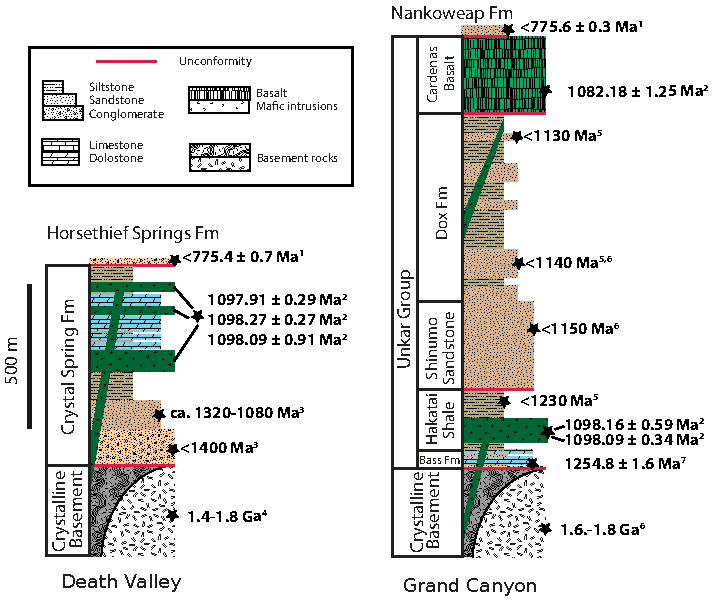
\includegraphics[width=\textwidth]{figure/Zhang2024b/DV_GC_Mesoproterozoic_strat_columns.pdf}
\caption[Simplified regional stratigraphy in Death Valley and Grand Canyon]{\footnotesize Simplified regional Mesoproterozoic stratigraphy in context of older basement rocks and younger Neoproterozoic sedimentary rocks and compiled geochronology in Death Valley and Grand Canyon. Red lines are unconformities. Black stars are existing radioisotopic age constraints. $^1$ CA-ID-TIMS U-Pb detrital zircon dates \citep{Dehler2023a}; $^2$ CA-ID-TIMS U-Pb zircon dates \citep{Mohr2024a}; $^3$ LA-MC-ICPMS U-Pb detrital zircon dates \citep{Mahon2014b}; $^4$ muscovite, biotite, and potassium feldspar $^{40}$K-$^{40}$Ar and $^{87}$Rb-$^{87}$Sr dates \citep{Lanphere1964b}, biotite, muscovite, and hornblende$^{40}$Ar-$^{39}$Ar dates \cite{Labotka1985a}, and SHRIMP U-Pb zircon and monazite dates \cite{Barth2001a, Barth2009a}; $^5$ \cite{Mulder2017a}; $^6$ detrital zircon and detrital muscovite dates \cite{Timmons2005a}; $^7$ TIMS U-Pb zircon dates from an ash layer \cite{Timmons2005a}.}
\label{fig:DV_GC_strat_columns}
\end{figure}

\subsection*{Mafic intrusions in the Unkar Group}

The Grand Canyon Supergroup is divided into the Mesoproterozoic Unkar Group and the Neoproterozoic Chuar Group \citep{Gundy1951a, Elston1989a, Dehler2017a}. The $\sim$2 km-thick Unkar Group contains the Bass Formation, Hakatai Shale, Shinumo Quartzite, Dox Formation, and Cardenas Basalt (Figure \ref{fig:DV_GC_strat_columns}; \citealp{Beus1974a, Elston1989a}). It is interpreted that the Unkar Group dominantly records shallow marine and fluvial depositional environments \citep{Elston1989a, Sears1990a, Hendricks1989a, Timmons2005a}. Siliclastic deposition continued during eruption of the Cardenas Basalt resulting in interflow siltstone and sandstones---often with mudcracks and current ripples respectively  (Fig. \ref{fig:cardenas_strat}). Unkar Group strata typically dip at $\sim$10\textdegree\ to the northeast (Figure \ref{fig:geologic_maps}) toward normal faults that dip $\sim$60\textdegree\ to the southwest \citep{Sears1973a, Timmons2012a}. Intraformational faults and large thickness changes in sedimentary units across faults indicate that the Unkar Group was deposited in an extensional tectonic setting \citep{Sears1990a, Karlstrom1998a, Timmons2001a}. 

Numerous mafic sills and dikes intrude the Unkar Group, but not the overlying Chuar Group (Figures \ref{fig:geologic_maps}B and \ref{fig:DV_GC_strat_columns}; \citealp{Elston1989a}). Sills typically intrude the Bass Formation and the Hakatai Shale of the lower Unkar Group \citep{Hendricks1989a} whereas mafic dikes have been mapped to crosscut the Shinumo Sandstone and the Dox Formation of the upper Unkar Group \citep{Timmons2012a}. Typical dike plane orientations are subparallel to NW-trending faults in the Unkar Group \citep{Huntoon1996a, Timmons2012a}. The sills typically range in thickness between 20 to over 100 meters and are alkali-olivine basalt in composition (\citealp{Hendricks1989a, Larson1994a}; Figure \ref{fig:geochem_major}). Given their spatial proximity and stratigraphic relationship, it had been commonly inferred that all mafic intrusions in the Unkar Group are feeders to the Cardenas Basalt \cite[e.g.][]{Huntoon1996a, Timmons2012a}, though no direct feeder relationships have been observed.

The interior of the thick mafic sills are medium- to coarse-grained with subophitic to ophitic texture characterized by plagioclase and olivine grains being enclosed by poikilitic pyroxenes \citep{Hendricks1989a}. The intrusions are fine-grained at their margins where they are chilled against the Unkar sedimentary rocks.  Some of the sill interiors contain zircon-bearing segregations \citep{Mohr2024a}, which were dated with high-precision CA-ID-TIMS $^{206}$Pb/$^{238}$U at 1098.16 $\pm$ 0.59 Ma at Hotauta Canyon (river mile [RM] 107) and 1098.09 $\pm$ 0.34 Ma at Stone Creek (RM 132) (Figure \ref{fig:SWLLIP_overview}B, \ref{fig:geologic_maps}B; 2$\sigma$ uncertainties). 

\subsection*{Cardenas Basalt}

The Cardenas Basalt at the top of the Unkar Group exclusively outcrops in eastern Grand Canyon (Figure \ref{fig:geologic_maps}). The most complete section of the Cardenas Basalt outcrops at the Basalt Canyon area where $\sim$315 meters of lava flows and associated interflow sedimentary rocks are preserved up to the unconformity between the volcanics and the overlying Nankoweap Formation (Figure \ref{fig:geologic_maps}B, \ref{fig:cardenas_strat}; \citealp{Lucchitta1983a, Hendricks1989a}). Cardenas Basalt also outcrops with variable thicknesses at localities including Lava Chuar Canyon and Nankoweap Canyon (Figure \ref{fig:geologic_maps}B, \ref{fig:cardenas_strat}). The lava flows are typically trachy-basaltic andesite in composition, overall having higher SiO$_2$ values than the mafic intrusions in the Unkar Group (Figure \ref{fig:geochem_major}; \citealp{Hendricks1989a, Larson1994a}).

\begin{figure}[h!]
\centering
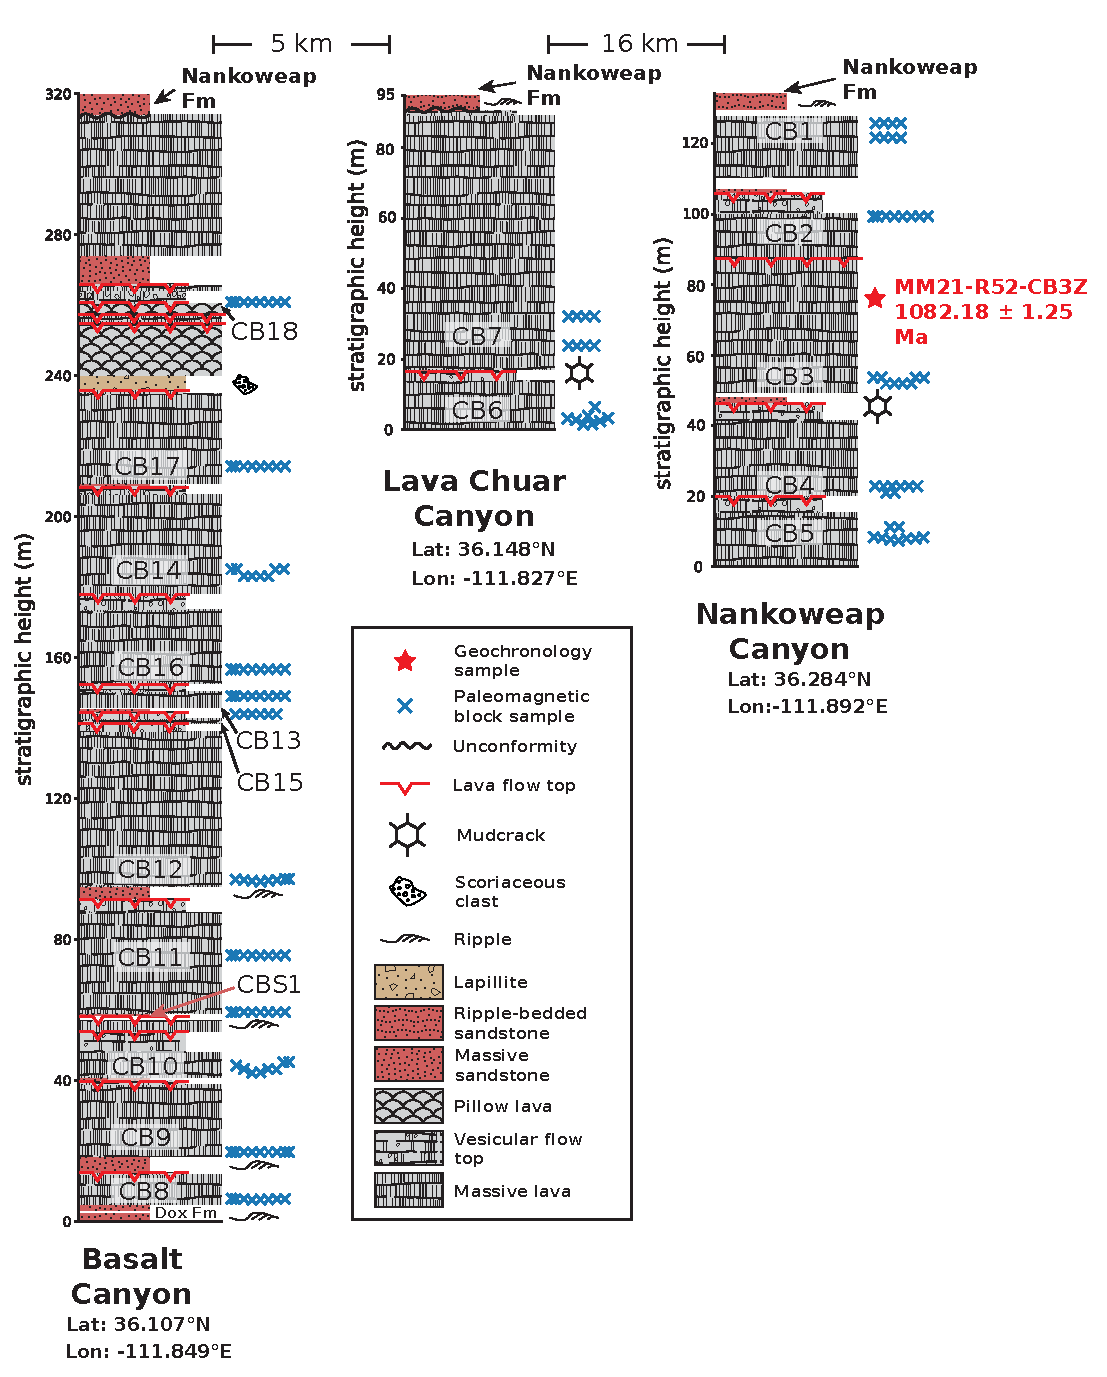
\includegraphics[width=0.82\textwidth]{figure/Zhang2024b/Cardenas_strat_uniform_scale.pdf}
\caption[Volcanostratigraphy of the Cardenas Basalt at Basalt Canyon, Lava Chuar Canyon, and Nankoweap Canyon]{Volcanostratigraphy of the Cardenas Basalt at Basalt Canyon, Lava Chuar Canyon, and Nankoweap Canyon measured in this study. Section locations are shown in Figure \ref{fig:geologic_maps}B. Stratigraphic locations of the collected paleomagnetic samples and the geochronology sample dated by \cite{Mohr2024a} are shown. The interflow sandstones and vesicular lava flow tops distinguish individual lava flows such that paleomagnetic samples from each lava flow constitute a site (labeled as `CB' with distinct numbers). The latitude and longitude values correspond to the base of the stratigraphic sections.}
\label{fig:cardenas_strat}
\end{figure}

Previous studies constructed volcanostratigraphic sections of the Cardenas Basalt at Basalt Cliffs, Ochoa Point, Basalt Canyon, and Lava Chuar Canyon \citep{Lucchitta1983a, Hendricks1989a}. In particular, \cite{Hendricks1989a} developed a stratigraphic section at Basalt Canyon with detailed petrologic and lithologic descriptions. In this study, we investigated three sections at Basalt Canyon, Lava Chuar Canyon, and Nankoweap Canyon (Figure \ref{fig:geologic_maps}). We measured volcanostratigraphic sections with a particular focus on determining individual lava flows that represent distinct cooling units such that paleomagnetic samples collected from a single lava flow are considered to capture the same snapshot of the geomagnetic field as they cooled (i.e. a paleomagnetic site; Fig. \ref{fig:cardenas_strat}). Flow boundaries can be delineated by progressive changes in vesiculation and by highly vesiculated flow tops and/or interflow clastic sedimentary rocks (Figure \ref{fig:cardenas_strat}, \ref{fig:field_photo}E). Interflow sedimentary rocks between lava flows are common (Figure \ref{fig:cardenas_strat}).

At Basalt Canyon, flows in the initial 95 meters are subophitic to ophitic in texture and heavily weathered with a greenish color (Figure \ref{fig:field_photo}B). These flows form slopes characterized by small weathered basalt fragments that often are dislodged pyroxene oikocrysts. Walking on steep slopes mantled by these oikocrysts is like walking on ball bearings. \cite{Walcott1883a} and \cite{Lucchitta1979a} noted that those flows experienced spilitic alteration, interpreted as the result of subaqueous eruptions in a tidal flat or deltaic environment. The claim has also been made that there are pillows in these lower flows \citep{Stevenson1982a, Hendricks1974a}. However, our field observations, as well as those of \cite{Larson1994a} and \cite{Elston1976a}, did not find evidence of pillow lava indicative of subaqueous eruptions in these flows---note that spheroidal weathering can often be misidentified as pillows. While spheroidal weathering, granular grus piles, and ophitic textures on the weathered exposures are common, the features in these basal ophitic flows, including the presence of an observed pahoehoe flow top and basal pipe vesicles, are consistent with them being subaerially erupted sheet flows (Figure \ref{fig:field_photo}B). A ropy flow top consistent with pahoehoe lava flows was also reported in \cite{Hendricks1989a}. The upper 200 meters of Cardenas Basalt flows consist of more competent, cliff-forming lava flows that are finer-grained than the lower sequence. A 4-meter-thick volcaniclastic layer containing cobble- to boulder-sized scoriaceous volcanic clasts surrounded by tan-colored, fine-grained matrix occurs at stratigraphic height of $\sim$240 m (Figure \ref{fig:cardenas_strat}, \ref{fig:field_photo}D). \cite{Lucchitta1983a} named this unit the lapillite member of the Cardenas Basalt and interpreted that it likely formed as pyroclastic debris deposited by lahars. Pillow lavas typically 0.8 to 1 m wide with horizons of volcaniclastic materials consistent with subaqueous eruption are found near the top of the section, above the lapillite layer (Figure \ref{fig:field_photo}F). 

Shorter sections of Cardenas Basalt flows are exposed in Nankoweap Canyon (RM 52) and Lava Chuar Canyon (RM 65) (Figure \ref{fig:geologic_maps}B, \ref{fig:cardenas_strat}). Due to the less complete exposures at these two localities, the volcanostratigraphic correlations between the three localities cannot be unequivocally drawn. However, large lateral variability of individual lava flow thicknesses has been reported \citep{Lucchitta1983a}, indicating that lava flows likely pinch out laterally between the localities. Our stratigraphic sections at the three localities also show variable lava flow thicknesses directly below the Nankoweap Formation (Figure \ref{fig:cardenas_strat}) although this could reflect variability in erosional truncation. We treat the sampled lava flows sampled at different localities as distinct cooling units in this study with each being an individual paleomagnetic site (Figure \ref{fig:cardenas_strat}). The \cite{Mohr2024a} geochronology sample for the Cardenas Basalts comes from the interior of a 57 m thick lava flow at Nankoweap Canyon (Figure \ref{fig:field_photo}A; CB3). Four zircon microlites yielded a weighted mean $^{206}$Pb/$^{238}$U ages of 1082.18 $\pm$ 1.25 Ma (95\% confidence; Figure \ref{fig:SWLLIP_overview}B). 

\begin{figure}[h!]
\centering
\includegraphics[width=0.82\textwidth]{figure/Zhang2024b/field_photo.png}
\caption[Field photos of Cardenas Basalt]{Field photos of Cardenas Basalt. The site names correspond to those shown in the stratigraphic section in Figure \ref{fig:cardenas_strat}. (A) Coarse-grained interior of the 57 m thick CB3 lava flow at Nankoweap Canyon from which zircon were extracted and dated by \cite{Mohr2024a}. (B) Ophitic texture in the interior of flow CB9 at Basalt Canyon. Individual oikocrysts reach diameters of 9 mm. (C) Contact between two individual lava flows CB14 and CB16 (meter level 178 in Fig. \ref{fig:cardenas_strat}) The massive flow bottom of the upper flow is more resistant to weathering than the recessive vesiculated flow top of the underlying flow. (D) The volcaniclastic marker bed containing scoriaceous volcanic clasts surrounded by tan-colored, very fine-grained matrix at 236 to 240 m in the Basalt Canyon section. (E) Amygdaloidal flow top of CB16. Elongate amygdules indicate that vesicles were stretched during flow. (F) Pillow lavas near the top of the exposed stratigraphy at Basalt Canyon (within interval from meter level 240 to 257; Fig. \ref{fig:cardenas_strat}). }
\label{fig:field_photo}
\end{figure}

\section*{Methods}

A total of 123 samples from 15 individual mafic sills were collected from the Death Valley region (Fig. \ref{fig:geologic_maps}A). Core samples were collected with a gasoline-powered drill outside of Death Valley National Park and block samples were collected from sills inside the park. In the Grand Canyon, a total of 184 block samples were collected from 18 individual Cardenas Basalt lava flows, 1 baked interflow sedimentary bed, and 5 mafic intrusions within the Unkar Group. When sampling the intrusions, we preferentially targeted the finer-grained margins of flows and intrusions over the coarser-grained interiors. Typically, 6-9 samples were collected at each site. Both magnetic compass and sun compass were used when orienting the drill cores and block samples in the field. Sun compass orientations were preferentially used when available. In the lab, standard paleomagnetic cores were drilled from the block samples and then oriented relative to the oriented surfaces.

The locations of the paleomagnetic sites are shown in Figure \ref{fig:geologic_maps} and Table \ref{tab:pmag_data}, and the stratigraphic positions of block samples collected from the Cardenas Basalt are shown in Figure \ref{fig:cardenas_strat}. In western Grand Canyon, we sampled the 1098.16 $\pm$ 0.59 Ma sill in Hotauta Canyon as UI4 (RM 107) and the 1098.09 $\pm$ 0.34 Ma Stone Creek Canyon sill as UI5 (RM 132). In the eastern canyon, we sampled the Hance dike north to the Hance Rapids (UI2; RM 77) and the Hance sill south to the rapids (UI3). Another undated mafic sill was sampled at Red Canyon (RM 77) which is south of the river at Hance Rapids along the tributary stream channel of Red Canyon (UI1; Figure \ref{fig:geologic_maps}B). In Death Valley, within Warm Spring Canyon, we sampled the 1097.91 $\pm$ 0.29 Ma sill as CS1 and the 1098.27 $\pm$ 0.27 Ma sill as CS4, and in Ibex Hills, we sampled the 1098.09 $\pm$ 0.91 Ma sill as CS7. Other undated sills are labeled in Figure (\ref{fig:geologic_maps}) and locations for all sites are available in the archived data repository (\url{https://zenodo.org/doi/10.5281/zenodo.10625967}). 

A suite of specimens from sills in the Crystal Spring Formation underwent step-wise thermal demagnetization up to 680 \textdegree C. An additional suite of sister specimens from some samples also underwent thermal demagnetization with an added step of a liquid nitrogen bath following the measurement of natural remanent magnetization. This demagnetization step can preferentially remove overprint magnetization held by multidomain titanomagnetite grains and potentially improve the resolution of the characteristic component. All specimens from the Cardenas Basalt and the mafic intrusions within the Unkar Group underwent step-wise thermal demagnetization up to 580 \textdegree C with some samples continuing up to 680 \textdegree C. The thermal demagnetization protocol had increasingly higher resolution approaching the Curie temperature of magnetite ($\sim$580\textdegree C) and N\'eel temperature of hematite ($\sim$680\textdegree C).

All demagnetization experiments were carried out in the magnetically shielded room at the UC Berkeley Paleomagnetism Lab. The typical magnetic field inside the shielded room is $<$500 nT. An ASC TD-48SC thermal demagnetizer with $<$10 nT field inside the chamber was used for the demagnetization steps. All remanence measurements were made on a 2G Enterprises DC-SQUID superconducting rock magnetometer. The PmagPy software package \citep{Tauxe2016a} was used to implement least-square fits \citep{Kirschvink1980a} to specimen demagnetization data. 

In the Death Valley region, multiple bedding orientations were measured along contacts between the sills and the host sedimentary rocks and along bedding of sedimentary rocks near the sills, and the averages of these measurements were used to tilt-correct paleomagnetic directions of each sill. In the Grand Canyon, the contact planes between the Hance sill and the adjacent sedimentary layers are poorly exposed. We collected bedding measurements from the nearby exposures of the Bass Formation for tilt correction. We also collected orientations from the Hance sill columnar joint planes---planes that are typically vertical prior to tilting. The best-fit plane orthogonal to the columnar joint planes has an orientation similar to the mean bedding plane of the Bass Formation. Bedding orientations of the host Hakatai Shale were used to tilt-correct the Hance dike paleomagnetic data. Bedding orientations were taken on the Cardenas Basalt flow tops and on interflow sediments for tilt correction. All bedding orientation data are available in the archived data repository (\url{https://zenodo.org/doi/10.5281/zenodo.10625967}).

\section*{Results and Interpretations}

Eight out of the 15 mafic sills from the Death Valley area yielded stable, consistent, and interpretable paleomagnetic directional data. All sites including 5 mafic sills, 18 lava flows, and 1 interflow sedimentary bed sampled in the Grand Canyon yielded well-grouped, consistent paleomagnetic directions. The site-level paleomagnetic statistics are summarized in Table \ref{tab:pmag_data}. Data to the individual measurement level are available in the MagIC database (private link for reviewer here: \url{https://doi. org/10.7288/V4/MAGIC/20009}).

\begin{sidewaystable}
\resizebox{0.95\textwidth}{!}{
\tiny
\begin{tabular}{p {1cm} p {2.5cm} p {1.5cm} p {2cm} p {2.3cm} p {0.5cm} p {1cm} p {1cm} p {1cm} p {1cm} p {1cm} p {1cm} p {1cm} p {1cm} }
\hline
site      & study region     & geologic type            & site latitude (\textdegree N) & site longitude (\textdegree E) & n  & dec$_{gc}$                    & inc$_{gc}$                   & dec$_{tc}$ & inc$_{tc}$ & k    & $\alpha_{95}$ (\textdegree) & vgp lat (\textdegree N) & vgp lon (\textdegree E) \\
\hline
CS1$^*$       & Death Valley & sill                 & 35.9688  & -116.9190 & 8  & 303.0                        &  50.0                        & 292.8   & 73.3    & 175  & 4.2  & 41.7     & 203.7    \\
CS2       & Death Valley & sill                 & 35.9651  & -116.9130 & 7  & 290.2                        & 43.2                        & 296.3   & 65.3    & 27   & 11.9 & 42.5     & 187.7    \\
CS6       & Death Valley & sill                 & 35.9618  & -116.8829 & 8  & 275.5                        & -4.7                        & 281.3   & 48.4    & 45   & 8.3  & 25.2     & 172.3    \\
CS7$^*$       & Death Valley & sill                 & 35.8154  & -116.3886 & 2  & 318.0                        & -8.0                        & 331.1   & 42.4    & 167  & 19.5 & 62.7     & 137.2    \\
CS8       & Death Valley & sill                 & 35.8114  & -116.3854 & 9  & 305.2                        & 5.2                         & 297.1   & 58.7    & 78   & 5.9  & 41.1     & 177.8    \\
CS9       & Death Valley & sill                 & 35.8112  & -116.3855 & 5  & 316.0                        & -2.0                        & 317.5   & 52.6    & 39   & 12.3 & 55.1     & 161.9    \\
CS12      & Death Valley & sill                 & 35.7789  & -116.1206 & 8  & 284.7                        & 2.3                         & 301.6   & 63.3    & 30   & 10.2 & 45.5     & 184.3    \\
CS13      & Death Valley & sill                 & 35.8187  & -116.0938 & 3  & 269.0                        & -13.7                       & 293.6   & 51.2    & 150  & 10.1 & 35.8     & 170.3    \\
CB1       & Grand Canyon & lava flow            & 36.2839  & -111.8919 & 8  & 249.3                        & 52.9                        & 270.3   & 51.1    & 200  & 3.9  & 18.4     & 184.5    \\
CB2       & Grand Canyon & lava flow            & 36.2836  & -111.8919 & 8  & 276.3                        & 56.5                        & 283.3   & 78.7    & 329  & 3.1  & 38.2     & 220.8    \\
CB3$^*$       & Grand Canyon & lava flow            & 36.2833  & -111.8928 & 7  & 261.3                        & 58.7                        & 249.3   & 52.9    & 56   & 8.1  & 5.1      & 196.5    \\
CB4       & Grand Canyon & lava flow            & 36.2831  & -111.8928 & 7  & 248.6                        & 35.0                        & 261.3   & 58.7    & 37.1 & 10.0 & 16.9     & 196.9    \\
CB5       & Grand Canyon & lava flow            & 36.2825  & -111.8914 & 9  & 241.6                        & 45.7                        & 276.3   & 56.5    & 71   & 6.2  & 25.3     & 186.8    \\
CB6       & Grand Canyon & lava flow            & 36.1458  & -111.8275 & 8  & 270.3                        & 51.1                        & 252.7   & 47.0    & 88   & 5.9  & 3.8      & 190.7    \\
CB7       & Grand Canyon & lava flow            & 36.1464  & -111.8269 & 8  & 283.3                        & 78.7                        & 269.9   & 42.5    & 106  & 5.4  & 14.1     & 178.5    \\
CB8       & Grand Canyon & lava flow            & 36.1072  & -111.8486 & 8  & 271.9                        & 53.0                        & 272.7   & 38.5    & 132  & 4.8  & 14.7     & 174.5    \\
CB9       & Grand Canyon & lava flow            & 36.1073  & -111.8493 & 8  & 264.6                        & 37.4                        & 283.6   & 27.3    & 96   & 5.7  & 19.3     & 162.3    \\
CB10      & Grand Canyon & lava flow            & 36.1075  & -111.8489 & 7  & 264.0                        & 32.3                        & 273.9   & 38.0    & 88   & 6.5  & 15.4     & 173.6    \\
CB11 \& CBS1 & Grand Canyon & lava flow: sediments & 36.1082  & -111.8489 & 13 & 278.1                        & 28.4                        & 268.3   & 69.5    & 93.2 & 4.3  & 27.2     & 206.5    \\
CB12      & Grand Canyon & lava flow            & 36.1100  & -111.8531 & 8  & 265.9                        & 37.1                        & 268.8   & 42.0    & 193  & 4.0  & 13.1     & 178.8    \\
CB13      & Grand Canyon & lava flow            & 36.1101  & -111.8542 & 7  & 259.9                        & 40.0                        & 267.0   & 6.1     & 107  & 5.9  & -0.6     & 162.4    \\
CB14      & Grand Canyon & lava flow            & 36.1108  & -111.8553 & 7  & 266.0                        & 4.6                         & 259.4   & 52.9    & 514  & 2.7  & 11.6     & 191.3    \\
CB15      & Grand Canyon & lava flow            & 36.1103  & -111.8533 & 6  & 247.4                        & 49.1                        & 263.3   & 45.7    & 89   & 7.1  & 10.7     & 184.1    \\
CB16      & Grand Canyon & lava flow            & 36.1100  & -111.8547 & 7  & 253.6                        & 42.8                        & 266.2   & 17.5    & 63   & 7.7  & 2.2      & 167.6    \\
CB17      & Grand Canyon & lava flow            & 36.1114  & -111.8553 & 8  & 263.2                        & 15.7                        & 264.8   & 49.3    & 253  & 3.5  & 13.5     & 185.9    \\
CB18      & Grand Canyon & lava flow            & 36.1117  & -111.8558 & 7  & 253.6                        & 46.5                        & 285.6   & 52.3    & 98   & 6.1  & 30.2     & 178.9    \\
UI1       & Grand Canyon & sill                 & 36.0247  & -111.9300 & 8  & 243.9                        & 66.1                        & 269.1   & 23.9    & 216  & 3.8  & 6.6      & 168.7    \\
UI2       & Grand Canyon & dike                 & 36.0456  & -111.9183 & 8  & 263.9                        & 19.3                        & 264.0   & 10.0    & 75   & 6.5  & -1.9     & 165.7    \\
UI3       & Grand Canyon & sill                 & 36.0458  & -111.9267 & 8  & 258.1                        & 20.4                        & 264.1   & 25.6    & 139  & 4.7  & 3.2      & 172.4    \\
UI4$^*$       & Grand Canyon & sill                 & 36.2353  & -112.3294 & 7  & 264.0                        & 14.3                        & 314.1   & 51.6    & 54   & 8.3  & 52.2     & 165.4    \\
UI5$^*$       & Grand Canyon & sill                 & 36.3483  & -112.4525 & 8  & 278.2                        & 49.2                        & 295.6   & 49.3    & 76   & 6.4  & 36.8     & 170.8   \\
\hline
\end{tabular}
}
\caption[Site-level paleomagnetic data from mafic sills in Death Valley, Cardenas Basalt, and mafic intrusions in the Unkar Group]{Site-level paleomagnetic data from mafic sills in Death Valley, Cardenas Basalt, and mafic intrusions in the Unkar Group. dec$_{gc}$ and inc$_{gc}$ are site mean declination and inclination in geographic coordinates. dec$_{tc}$ and inc$_{tc}$ are site mean declination and inclination in tilt-corrected coordinates. k represents the Fisher concentration parameter of the site level mean directions. $\alpha_{95}$ represents the Fisher 95\% angular uncertainty of the site level mean directions. \textit{vgp lat} and \textit{vgp lon} represent the latitude and longitude of the site-level virtual geomagnetic poles calculated from tilt-corrected directional data. $^*$ marks sites that have paired high-precision zircon U-Pb ages developed by \cite{Mohr2024a}. CS1 is dated to be 1097.91 $\pm$ 0.29 Ma; CS7 is dated to be 1098.09 $\pm$ 0.91 Ma; UI4 is dated to be 1098.16 $\pm$ 0.59 Ma; UI5 is dated to be 1098.09 $\pm$ 0.34 Ma. All ages are presented with 95\% confidence. }
\label{tab:pmag_data}
\end{sidewaystable}

\subsection*{Death Valley mafic sills}
Thermal demagnetization results on specimens with stable and consistent remanence from the Death Valley sills show that the specimens typically have an overprint component (Figure \ref{fig:demag_plots}). That component can be removed by heating up to $\sim$500\textdegree C, although it is largely removed after heating to 100\textdegree C. The liquid nitrogen demagnetization step (77 K) was also efficient in removing this component. Following the removal of the secondary component, an origin-trending component was resolved through the progressive thermal demagnetization steps up to the Curie temperature of magnetite (i.e. $\sim$580\textdegree C; Figure \ref{fig:demag_plots}).

In geographic coordinates, the site level low-temperature component directions of the Death Valley sills lie very close to the direction of the present-day geomagnetic field direction in Death Valley (Figure \ref{fig:demag_plots}). The low unblocking temperature and the directions of this component are consistent with it being a geologically recent viscous remanence overprint \citep{ Moskowitz1998a, Muxworthy2000a}. On the other hand, the origin-trending component in the sills removed at higher temperatures is directed to the northwest with steep downward inclinations after tilt correction (Figure \ref{fig:demag_plots}). Eight sills yielded consistent results within site and well-grouped mean directions amongst sites. The other sills failed to yield resolvable characteristic directions or consistent results within sites. Figure \ref{fig:poles}A shows the virtual geomagnetic poles (VGP) and the mean pole position (pole longitude=176.6\textdegree, pole latitude=44.9\textdegree, n=8, A$_{95}$=11.8\textdegree; no rotation correction) calculated from the tilt-corrected sills in Death Valley.

\begin{figure}[h!]
\centering
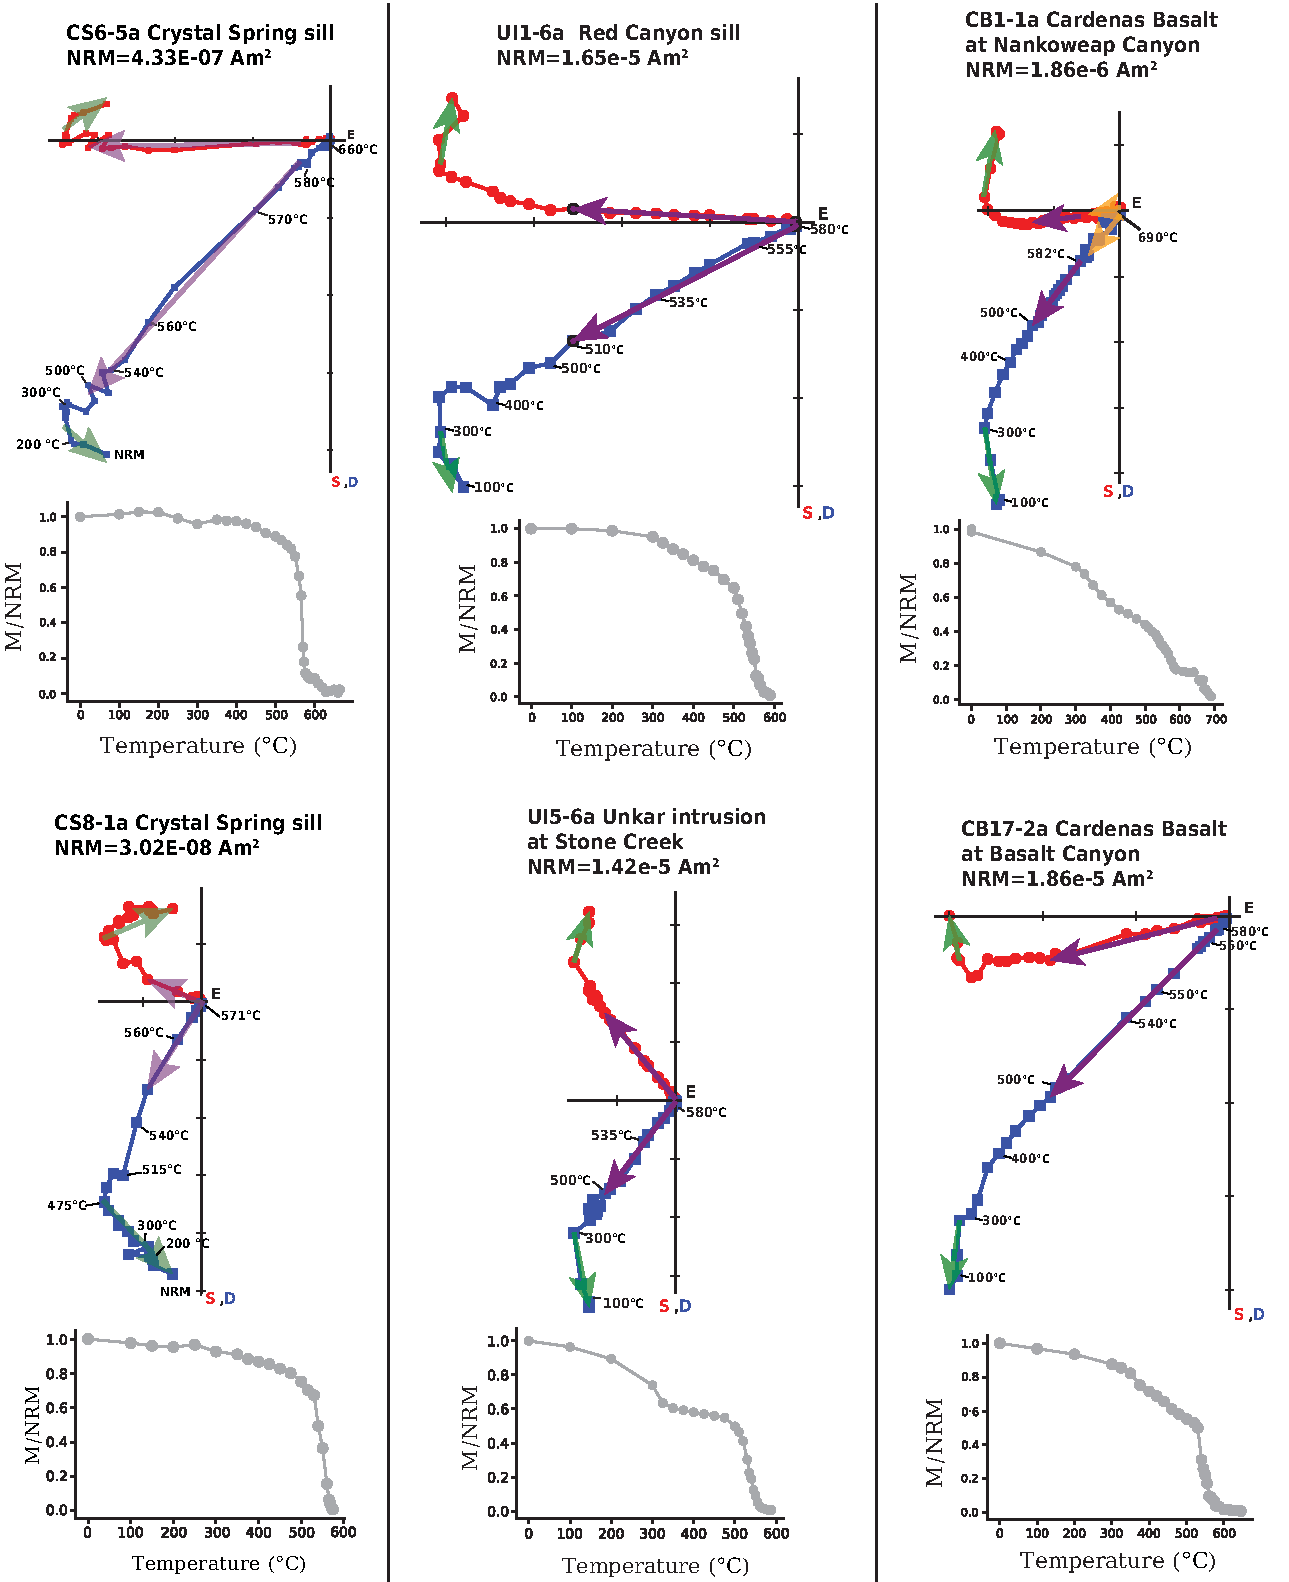
\includegraphics[width=0.78\textwidth]{figure/Zhang2024b/demag_plots.pdf}
\caption[Example orthogonal vector diagrams of specimen thermal demagnetization results]{\footnotesize Example orthogonal vector diagrams of specimen thermal demagnetization results from mafic sills that intruded the Crystal Spring Formation, mafic sills that intruded the Unkar Group, and the Cardenas Basalt. Total specimen magnetic moments (M) normalized by the natural remanent magnetizations (NRM) are plotted against temperature steps. The secondary overprint component (green) in the rocks can be removed by heating typically to $\sim$300\textdegree C, but can be up to $\sim$500\textdegree C, or efficiently removed by liquid nitrogen demagnetization. The interpreted primary component (purple) is origin-trending and typically unblocks sharply through $\sim$500-580\textdegree C. In some Cardenas lava flows such as CB1, a third component that unblocks up to $\sim$690\textdegree C exists, and is interpreted to be carried by hematite that formed during early oxidation. All orthogonal plots are shown in tilt-corrected coordinates.}
\label{fig:demag_plots}
\end{figure}

\subsection*{Intrusions in the Unkar Group and the Cardenas Basalt}
The two dated ca. 1098 Ma sills in eastern Grand Canyon (UI4 and UI5) and three intrusions near Hance Rapids and in Red Canyon (UI1, UI2, and UI3; Figure \ref{fig:geologic_maps}B) all yielded consistent within-site thermal demagnetization results and have similar thermal demagnetization behaviors between sites (Figure \ref{fig:demag_plots}, \ref{fig:equal_area_plots}). Typically, an origin-trending characteristic remanence component unblocks between 500\textdegree C and 585\textdegree C after a secondary overprint component that overlaps with the present local field direction is removed at lower temperatures (Figure \ref{fig:demag_plots}). This thermal demagnetization behavior indicates that the characteristic remanence components in these mafic intrusions are held by low-titanium titanomagnetite. Despite their similar demagnetization behaviors, the mafic intrusions record two distinct groups of remanence directions (Figure \ref{fig:equal_area_plots}). The ca. 1098 Ma mafic sills in Hotauta Canyon (UI4) and Stone Creek Canyon (UI5) record paleomagnetic directions to the northwest with steep inclinations, whereas the other three undated intrusions in eastern Grand Canyon have westerly directions and much shallower inclinations (Figure \ref{fig:demag_plots}, \ref{fig:equal_area_plots}). 

Thermal demagnetization of the 18 Cardenas Basalt lava flows yielded consistent site-level results (Figure \ref{fig:equal_area_plots}). After an overprint component that overlaps with the present local field direction was removed by heating up to 300\textdegree C (Figure \ref{fig:demag_plots}), the specimens typically demagnetized along an origin-trending path approaching the Curie temperature of magnetite. Some specimens continued to demagnetize up to the N\`eel temperature of hematite ($\sim$690\textdegree C; \cite{Ozdemir2006a}; Figure \ref{fig:demag_plots}). The unblocking temperature ranges indicate that (titano)magnetite and hematite are the dominant remanence-carrying minerals in the lava flows. Least-squares line fits made for the magnetite and hematite components have very similar directions in the same specimens (Figure \ref{fig:demag_plots}; CB1-1a). This result is consistent with the hematite having formed due to early oxidation of the lava flows indicating that it acquired remanent magnetization soon after the eruption of the lavas. 

\begin{figure}[h!]
\centering
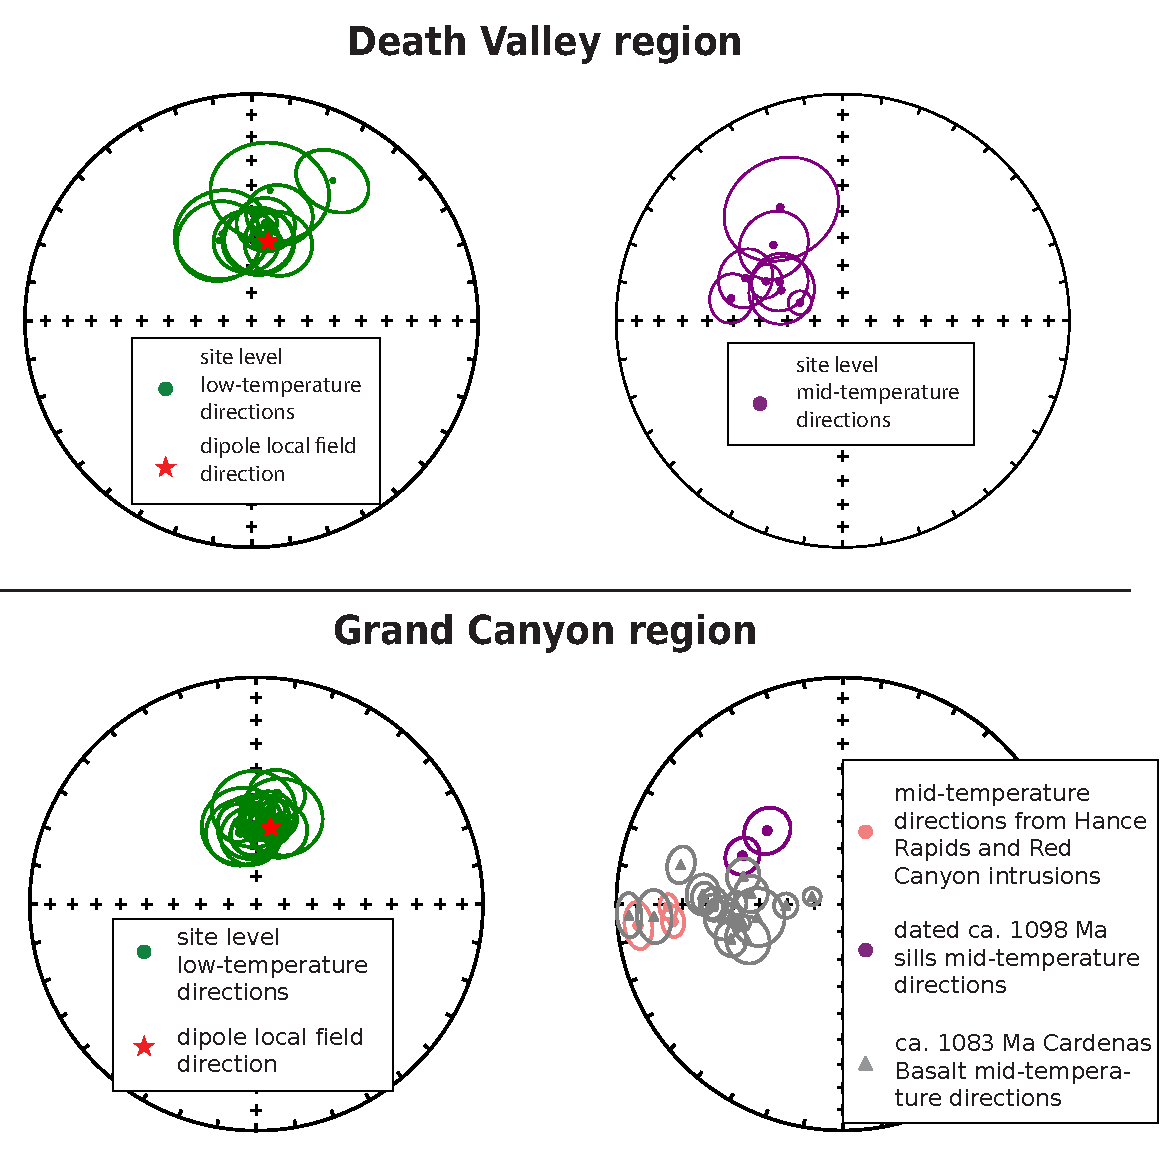
\includegraphics[width=0.8\textwidth]{figure/Zhang2024b/equal_area_plots.pdf}
\caption[equal area diagrams for the site level directional results from the Death Valley region and the Grand Canyon region]{\footnotesize Summary equal area diagrams for the site level directional results from the Death Valley region and the Grand Canyon region. The site level low-temperature components (green) in geographic coordinates are shown in context of present-day local field directions (red star) at the study localities. The mid-temperature directions (i.e. those that unblock over a temperature range consistent with magnetite) are shown in tilt-corrected coordinates. Note that the specimen directions from the mafic sills at Hotauta Canyon (UI4) and Stone Creek (UI5) (directions shown in purple) are more northerly and steeper than the specimen directions of Cardenas Basalt and the intrusions near Hance Rapids (shown in grey and pink).}
\label{fig:equal_area_plots}
\end{figure}

Site-level characteristic directions for all of the intrusions in Death Valley and Grand Canyon as well as Cardenas Basalt flows except for CB4 were calculated using the (titano)magnetite-bearing components. This component isolated through magnetite unblocking temperatures is referred to as the ``mid-temperature direction" in Figure \ref{fig:equal_area_plots}. For site CB4, all except for one specimen have antipodal components, both of which we interpret to be carried by hematite. The antipodal directions recorded within the same specimens may be the result of magnetic self-reversal associated with the oxidation of magnetite into maghemite which subsequently inverted into hematite \citep{Swanson-Hysell2011a}. A detailed description of the specimen results for site CB4 is presented in Figure \ref{fig:CB4_reversal_test}. We combine the normal-polarity (i.e. directions pointing southwest and down) directions held by hematite in six samples together with a normal polarity direction carried by titanomagnetite in one sample for calculating a site mean direction for this flow. Seven samples collected from a baked interflow red sandstone layer (site CBS1) within 0.2 m of the base of lava flow CB11 yielded overlapping paleomagnetic directions with those from the overlying lava flow (Figure \ref{fig:SI_CBS1_CB11}). We group the samples from the lava flow and the baked sediments as one site when calculating the mean direction and virtual geomagnetic pole (VGP). Figure \ref{fig:poles}B shows the VGPs of the two dated ca. 1098 Ma sills in eastern Grand Canyon (UI4 and UI5), VGPs of the the Cardenas Basalt sites, the mean pole position calculated for the Cardenas Basalt (pole longitude=183.9\textdegree, pole latitude=15.9\textdegree, N=18, A$^{95}$=7.4\textdegree, K=22.7; no rotation correction) and the VGPs of the intrusions near Hance Rapids and Red Canyon (UI1, UI2, and UI3). 

\section*{Discussion}

\subsection*{Timing of mafic magmatism in the SWLLIP}

Statistically indistinguishable high-precision U-Pb zircon ages from three sills in Death Valley, two sills in the Grand Canyon, and a sill in central Arizona were interpreted in \cite{Mohr2024a} to be consistent with decompression melting of an upwelling mantle plume ca. 1098 Ma. This hypothesis predicts that other thick sills in the region associated with the SWLLIP were also emplaced ca. 1098 Ma. Paleomagnetic directional data can provide another avenue to gain chronological insight on mafic units for which geochronology data have not been or cannot be developed. Rapid changes in Laurentia's pole position between ca. 1110 and 1070 Ma (Fig. \ref{fig:poles}D; \citealp{Swanson-Hysell2019a}) enable such data to provide more informative temporal constraints than at many other time intervals.

The new paleomagnetic data from the dated sills in the Death Valley region and in the Grand Canyon are consistent with their high-precision U-Pb zircon ages. The 1097.91 $\pm$ 0.29 Ma CS1 sill  and the 1098.09 $\pm$ 0.91 Ma CS7 sill in Death Valley and the 1098.16 $\pm$ 0.59 Ma UI4 sill and 1098.09 $\pm$ 0.34 Ma UI5 sill in Grand Canyon have similar VGP positions at high latitudes in present-day coordinates (Figure \ref{fig:poles}A, B). The new paleomagnetic data further show that six additional undated sills in the Death Valley region have directions that are similar to those from the ca. 1098 Ma dated sills (Figs. \ref{fig:equal_area_plots} and \ref{fig:poles}). These data are consistent with all of the preserved Death Valley sills being associated with the ca. 1098 Ma pulse of mafic magmatism. Figure \ref{fig:poles}A shows the mean pole position calculated for all the Death Valley region sills. The pole overlaps within uncertainty with the pole position of the ca. 1096 Ma North Shore Volcanic Group upper southwest sequence of the Midcontinent Rift (Figure \ref{fig:poles}A; \citealp{Swanson-Hysell2019a}). Although the paleomagnetic data of the Death Valley sills have directional uncertainties associated with potential vertical axis block rotations as detailed in the following section, these structural complexities do not take away the interpretation that the steep downward inclinations (Figure \ref{fig:demag_plots}) are compatible with a ca. 1098 Ma age. Additionally, the normal polarity of the magnetizations is consistent with the sills being emplaced during the earliest portion of the ca. 1099 to $<$1075 Ma Portage Lake normal polarity zone \citep{Swanson-Hysell2019a}---a late Mesoproterozoic superchron \citep{Driscoll2016b}. 

\begin{figure}[h!]
\centering
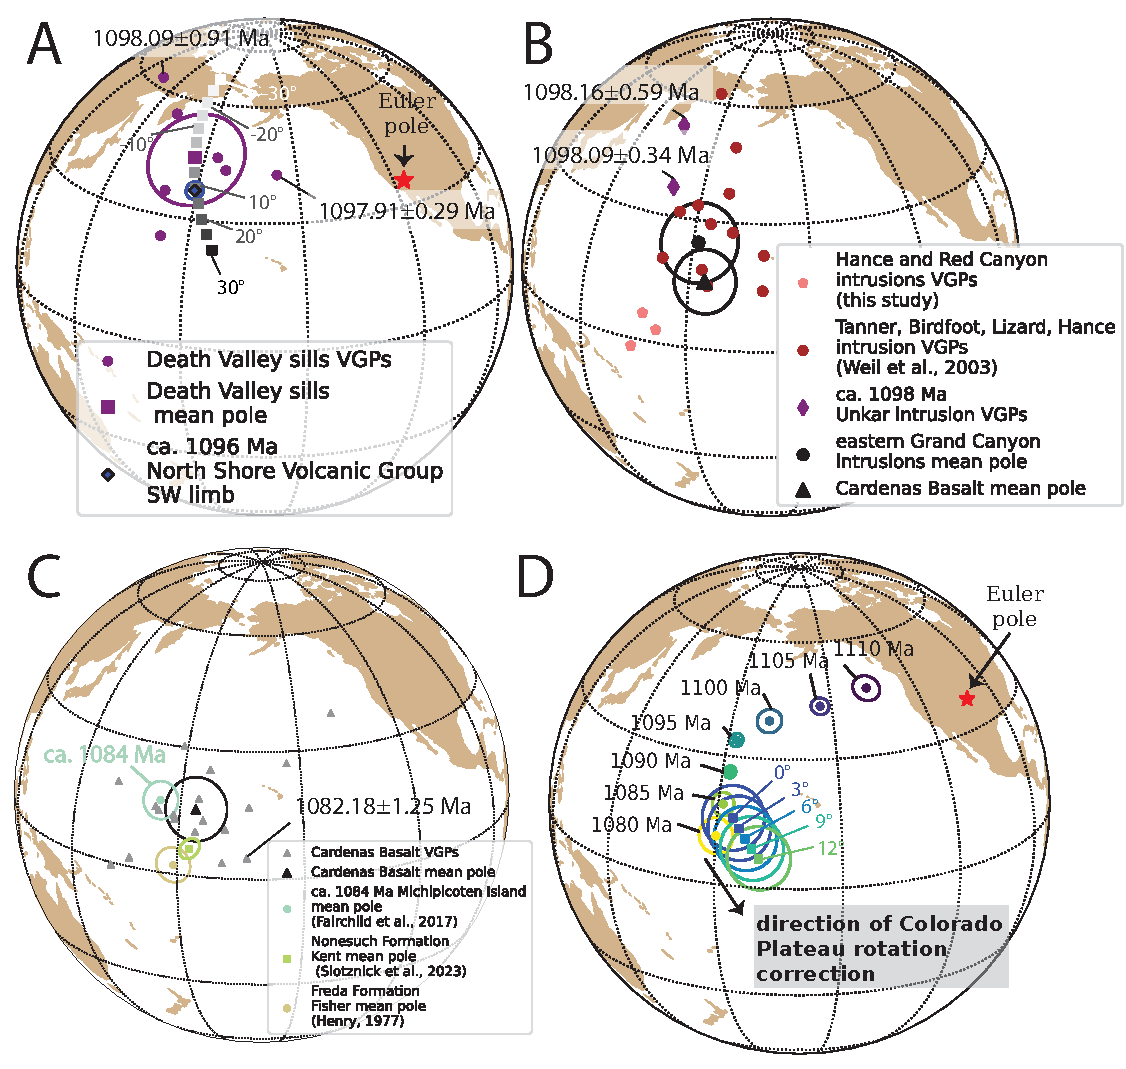
\includegraphics[width=0.8\textwidth]{figure/Zhang2024b/poles.pdf}
\caption[Pole positions of the Death Valley mafic sills, mafic intrusions in the Unkar Group, and the Cardenas Basalt]{\footnotesize (A) Virtual geomagnetic poles (VGP) from the Death Valley mafic sills and the associated mean paleomagnetic pole plotted in context of the paleomagnetic pole position of the ca. 1096 Ma North Shore Volcanic Group southwest sequence pole from \cite{Swanson-Hysell2019a}. Variable vertical axis rotations of the mean Death Valley sills pole about an Euler pole located at 35.8\textdegree N, -116.4\textdegree E are shown. Positive (negative) values represent counterclockwise (clockwise) rotations about the Euler pole. (B) VGPs from the Cardenas Basalt and mafic sills within the Unkar Group are plotted together with the mean Cardenas Basalt pole and the mean pole calculated for intrusions that are hypothesized to be coeval with the Cardenas Basalt. VGPs of intrusions include those developed in this study as well as those from \cite{Weil2003a}. (C) The mean ca. 1082 Ma Cardenas Basalt paleomagnetic pole is plotted together with the ca. 1084 Ma Michipicotan Island Formation paleomagnetic pole \citep{Fairchild2017a} as well as the ca. 1075 Ma Nonesuch Formation pole \citep{Slotznick2023a} and lower Freda Formation pole \citep{Henry1977a}. (D) The Cardenas Basalt mean pole position is corrected for the hypothesized Colorado Plateau rotation with progressively larger rotations about an Euler pole position of -107\textdegree E, 37\textdegree N \citep{Bryan1990a}. The resultant pole positions are plotted in context of the synthesized Keweenawan Track (2 stage pole rotations and true polar wander scenario; \citealp{Swanson-Hysell2019a}). Larger rotations result in less agreement between the Cardenas pole and the pole path based on Midcontinent Rift data. In plots (A) and (C) the VGPs from dated sills and the dated lava flow are labeled with their ages.}
\label{fig:poles}
\end{figure}   

The paleomagnetic pole position of the ca. 1082 Ma Cardenas Basalt plots at a lower latitude distinct from that of the ca. 1098 Ma mafic sills in Death Valley and the western Grand Canyon (Figure. \ref{fig:poles}A, C). Instead, the Cardenas Basalt pole is close to the paleomagnetic pole of the Michipicoten Island Formation of the Midcontinent Rift whose age is tightly bracketed to be between 1084.35 $\pm$ 0.20 Ma and 1083.52 $\pm$ 0.23 Ma \citep{Fairchild2017a}. In addition, the Cardenas Basalt pole is close to the ca. 1075 Ma paleomagnetic poles of the Nonesuch and Freda Formations \citep{Henry1977a, Slotznick2023a} of the Midcontinent Rift Oronto Group. That these localities $\sim$2,500 km apart yield overlapping pole positions when their poles are calculated under the assumption of a time-averaged dipolar field supports interpretations that the field was a stable dipole ca. 1080 Ma. Note that there is uncertainty in the Cardenas pole position associated with hypothesized rotation of the Colorado Plateau in the Mesozoic/Cenozoic (Fig. \ref{fig:poles}D; \citealp[e.g.][]{Bryan1990a}). However, this uncertainty does not take away from the main conclusion as it does not affect interpretations of paleolatitude.

Overall, the large arc distance between the ca. 1098 Ma and the ca. 1082 Ma poles from southwestern Laurentia supports the interpretation based on Midcontinent Rift data that Laurentia experienced rapid plate motion from high latitudes toward the equator in the late Mesoproterozoic \citep{Davis1997a, Swanson-Hysell2009a}. This rapid motion is associated with the closure of the Unimos Ocean which culminating in the onset of Grenvillian collisional orogenesis \citep{Swanson-Hysell2023a}. 

\subsection*{Comparison to Mesoproterozoic paleomagnetic data from central Arizona}

Paleomagnetic data have been developed from mafic sills in central Arizona that intrude the Apache Group sedimentary rocks \citep{Helsley1972a, Harlan1993a, Donadini2011a}. Both \cite{Harlan1993a} and \cite{Donadini2011a} identified sills in the same region that record normal directions and reversed directions with the reversed directions having steeper inclinations. We compiled paleomagnetic data from these two studies with the goal of having each site be a distinct cooling unit. The resultant compilation is provided in Table \ref{tab:SI_Harlan_Donadini_compilation}. The individual site-level directions, corresponding virtual geomagnetic pole positions, and overall mean directions and poles are recalculated by polarity and plotted in Figure \ref{fig:Harlan_Donadini_compilation}. 

The compiled mean pole position of the normal-polarity mafic sills in central Arizona plots near the expected pole position of Laurentia ca. 1095 Ma based on data from the Midcontinent Rift rocks (Figure \ref{fig:Harlan_Donadini_compilation}; \citealp{Swanson-Hysell2019a}). However, the distribution of the normal-polarity virtual geomagnetic pole positions is distinct from a Fisher distribution \citep{Fisher1953a}. Given that these VGPs show an elongate distribution along the Keweenawan Track (Figure \ref{fig:Harlan_Donadini_compilation}), we hypothesize that not all sills were emplaced during the same magmatic episode. However, that the sills have record a normal polarity and one sill yielded a U-Pb baddeleyite age of 1088 $\pm$ 11 Ma \citep{Bright2014a} which has an uncertainty that overlaps with an CA-ID-TIMS zircon U-Pb age of 1097.97 $\pm$ 0.12 Ma from a subhorizonal diabase sill in Salt River Canyon \citep{Mohr2024a} indicate that some of the sills could be coeval with the ca. 1098 Ma mafic sills in Death Valley and Grand Canyon. More precise radiometric dates that is paired with paleomagnetic data are needed from these sills. 

Despite the few records, the central Arizona sills with steep negative inclinations have a mean pole position distinct from that of the normal-polarity sills (Figure \ref{fig:Harlan_Donadini_compilation}). The mean pole plots near the older end of the Keweenawan Track, indicating a high paleolatitude for Laurentia at the time (Figure \ref{fig:Harlan_Donadini_compilation}). This configuration corresponds with the stable high-latitude position of Laurentia between ca. 1140 and 1105 Ma \citep{Ernst1993a, Piispa2018a, Swanson-Hysell2021c}. That reversed polarity is also consistent with the Alona Bay reversed polarity zone which has been identified during the onset of magmatism in the Midcontinent Rift \citep{Swanson-Hysell2019a}. The potential exists that in addition to there being a linkage between a SWLLIP plume that spread to the Midcontinent Rift ca. 1098 to 1096 Ma as hypothesized in \cite{Mohr2024a}, a plume upwelling under Laurentia at the onset of Midcontinent Rift development led to magmatism in both regions. To assess such temporal and dynamic connections, more precise ages of these reversed-polarity sills need to be determined. 

\begin{figure}[h!]
\centering
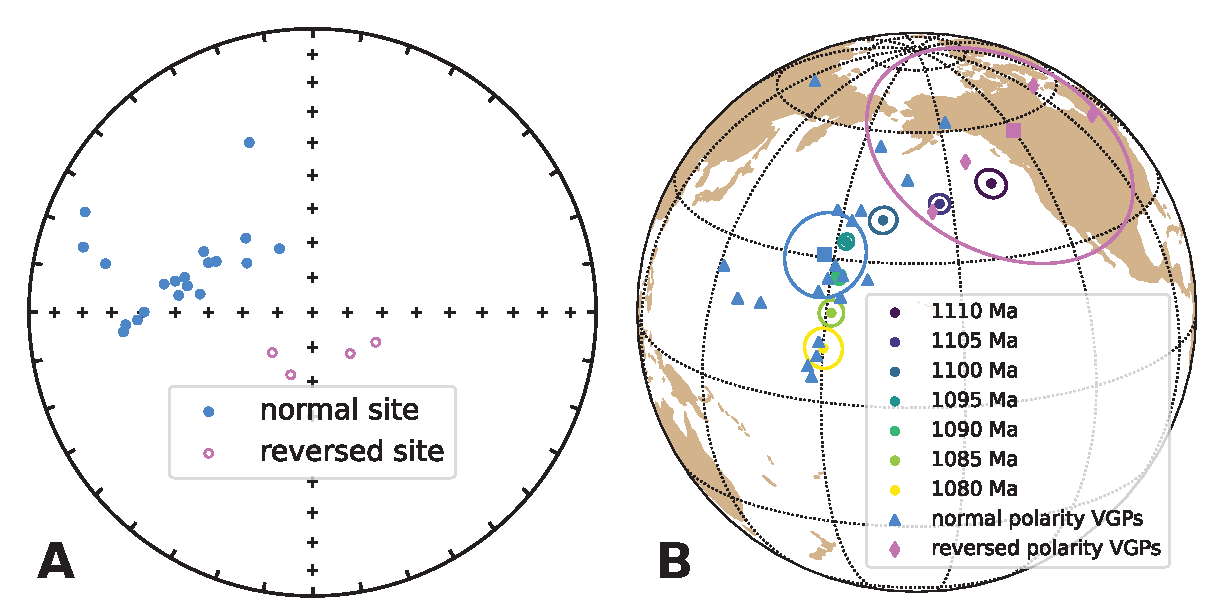
\includegraphics[width=0.8\textwidth]{figure/Zhang2024b/Harlan_Donadini_compilation.pdf}
\caption[Compilation of paleomagnetic data from central Arizona mafic sills]{(A) Compiled paleomagnetic directional data developed by \cite{Harlan1993a} and \cite{Donadini2011a} from mafic sills in central Arizona. The original data are selected with some recalculated such that each site included in this compilation is an individual cooling unit. Some sills record a reversed polarity with steep inclinations (orchid), while the other sills record a normal polarity with shallower inclinations (blue). The compiled data are in Table \ref{tab:SI_Harlan_Donadini_compilation}. (B) Virtual geomagnetic poles (VGP) of individual cooling units and mean paleomagnetic poles of the central Arizona mafic sills are plotted in context of the synthesized Keweenawan Track of \cite{Swanson-Hysell2019a} (two stage pole with true polar wander scenario). The mean pole position of sills with reversed polarity is close to the older end of the Keweenawan Track while the mean normal-polarity pole plots close to the expected pole position ca. 1095 Ma.}
\label{fig:Harlan_Donadini_compilation}
\end{figure}

\subsection*{Death Valley region sills}
\subsubsection*{Structural complexity associated with Neogene extension}

The Death Valley region experienced complex deformation associated with extension and shearing during Neogene extensional tectonism \cite[e.g.][]{Wernicke1988a}. It has been suggested that tilting associated with generally west-dipping normal faults, as well as vertical axis rotations of crustal blocks associated with conjugate strike-slip fault systems principally accommodated the deformation \cite[e.g.][]{Serpa1996a}. Geologic mapping and associated structural analyses suggest that strike-slip faults are coeval with normal faulting and have a left-lateral sense when they strike eastward or northeastward (e.g., Garlock fault; Figure \ref{fig:geologic_maps}A) and a right-lateral sense when they strike northwestward (e.g., south Death Valley fault;  Figure \ref{fig:geologic_maps}A); \citealp{Wright1976a, Serpa1996a, Pavlis2014a}). However, the extent to which extension is partitioned between the normal faulting and strike-slip faulting have long been debated \cite[e.g.][]{Burchfiel1965a, Guth1981a, Snow1989a, Holm1993a, Petronis2002a, Renik2013a}. 

The Death Valley region mafic sills that we sampled belong to different range-scale crustal blocks, including the Panamint Mountains, the Black Mountains, and the Nopah Range (Figure \ref{fig:geologic_maps}A). Sedimentary strata in the Crystal Spring Formation in these ranges dip variably to the east (Figure \ref{fig:geologic_maps}A). The mafic sills intruded parallel to the bedding of the Crystal Spring Formation, often taking advantage of contacts between different lithologies such as the contact between the argillite facies and the cherty dolomite facies. The dips of the sills vary between $\sim$23\textdegree to $\sim$86\textdegree. The paleomagnetic directions for the sills are much better grouped when corrected for this tilt (dec=302.8\textdegree, inc=58.0\textdegree, n=8, a$_{95}$=9.5\textdegree, k=34.8) than when considered in geographic coordinates without tilt correction (dec=295.1\textdegree, inc=8.9\textdegree, a$_{95}$=21.6\textdegree, k=7.5) (Figure \ref{fig:DV_tilt_test}). This result is consistent with the interpretation that the characteristic remanence component carried by (titano)magnetite in the sills is a primary remanence acquired during initial cooling prior to tilting of the Crystal Spring Formation. 

It is more challenging to correct for vertical axis rotations in the Death Valley region as the degrees of rotations are poorly constrained. Sills CS1, CS2, and CS6 are from Warm Spring Canyon of the Panamint Mountains, which is an east-tilting block now bounded by the right-lateral Panamint Valley fault to the west and the left-lateral Garlock fault to the south (Figure \ref{fig:geologic_maps}; \citealp{Snow1989a, Snow2000a}). \cite{Stewart1983a} interpreted that the Panamint Range was detached from above the crystalline core of the Black Mountains and translated some 80 km northwest along west dipping low-angle detachment faults. \cite{Petronis2002a} developed paleomagnetic data from Miocene intrusive rocks in the central Panamint Range and Miocene volcanic rocks in the eastern part of the range. Their data from the central range show a pole position that overlaps with that expected for no rotation, which they interpreted to indicate minimal amount of vertical axis rotation. They did find a discordance between paleomagnetic declinations developed from Miocene volcanic rocks in the eastern Panamint Range which appear to show substantial clockwise vertical axis rotations since the Miocene (27.6\textdegree\ $\pm$ 15.2\textdegree, calculated based on nine paleomagnetic sites). However, \cite{Petronis2002a} cautioned against interpreting there to have been a large vertical axis rotation in the eastern range as their data may undersample paleosecular variation. In the northwest Black Mountains, paleomagnetic data developed from Miocene intrusive rocks and Proterozoic basement rocks have been interpreted to indicate large vertical axis rotations as a result of oroclinal bending associated with right-lateral shear along the Death Valley fault zone (up to $\sim$80\textdegree; \citealp{Holm1993a}). However, paleomagnetic data developed from late Miocene igneous rocks in the eastern Panamint Mountains indicate minimal rotations in the region \citep{Petronis2002a}. These data led \cite{Petronis2002a} to hypothesize that the significant vertical axis rotation observed by \cite{Holm1993a} could be restricted to the western range where the basement block is sheared along the Death Valley fault zone (Figure \ref{fig:geologic_maps}). In this case, the more southeastern parts of the Black Mountains fault block, where sills CS7, CS8, and CS9 were collected, and distal from the fault zone, may have experienced relatively insignificant vertical axis rotation (Figure \ref{fig:geologic_maps}). In the Nopah Range, where site CS13 was sampled within the crystalline basement (Figure \ref{fig:geologic_maps}), no quantitative constraints exist on the amount of vertical axis rotation. Models that involve no rotation to those with up to 30\textdegree\ of clockwise rotation since the Neogene have all been proposed and interpreted to broadly fit the structural evidence in the region \cite[e.g.][]{Serpa1996a, Pavlis2014a}. Rotation in the Alexander Hills (site CS12) is similarly poorly constrained. 

The limited number of paleomagnetic sites from mafic sills in the different range blocks preclude the assessment of vertical axis rotation at each sampling locality (Figure \ref{fig:geologic_maps}A). This limitation is due to the secular variation of the geomagnetic field, which makes it such that single VGPs or low numbers of VGPs do not give accurate or precise estimate of the mean paleomagnetic pole position to be compared to a reference path. However, the tilt-corrected VGPs from the eight mafic sills with well-resolved magnetizations can provide insights into the structural history of the study region when viewed in context of Laurentia's apparent polar wander path in the late Mesoproterozoic. The tilt-corrected virtual geomagnetic poles from all sills are grouped at northern high latitudes, and the mean pole position plots close to the inverted pole position for ca. 1100 Ma and 1095 Ma (Figure \ref{fig:poles}A; \citealp{Swanson-Hysell2019a}). This position is consistent with the ca. 1098 Ma age given by the indistinguishable zircon U-Pb ages from the three dated sills (Figure \ref{fig:SWLLIP_overview}B; \citealp{Mohr2024a}). The overlapping pole positions between the Death Valley sills mean pole and poles from rocks of similar age in the Midcontinent Rift of the continental interior indicate that any vertical axis rotations were not large enough to have displaced the pole from the path ($<$30\textdegree\ ; Figure \ref{fig:poles}A).

Until more detailed and quantitative spatial and temporal constraints are developed for the different range blocks of the Death Valley region, it remains inconclusive as to the amount of Neogene vertical axis rotation correction to apply to these Mesoproterozoic sill directions. Given these vertical axis rotation uncertainties, we believe it is the best to not include the Death Valley mafic sills paleomagnetic pole into curated paleogeography databases. Nevertheless, the pole with no vertical axis rotations to the sites is consistent with the expected ca. 1098 position of Laurentia.

\subsection*{Grand Canyon region intrusions and Cardenas Basalt}

\cite{Weil2003a} developed paleomagnetic data from 13 mafic intrusions (in the eastern Grand Canyon between RM68 and RM78; Fig. \ref{fig:geologic_maps}) as well as three Cardenas Basalt flows at Basalt Canyon. Using the framework that the intrusions were time-equivalent with one another and with the lavas, \cite{Weil2003a} grouped all paleomagnetic directions from the intrusive and extrusive rocks to calculate a mean paleomagnetic pole position. There is an overall consistency in the directions of those studied units which is consistent with this interpretation. The pole was assigned an age of 1090.6 $\pm$ 4.5 Ma based on an $^{40}$Ar/$^{39}$Ar age developed from biotite collected within Unkar sedimentary rocks baked by a sill in the western Grand Canyon at RM131 (outside their paleomagnetic study region; \citealp{Weil2003a}). This mean pole position has been included in pole compilations \cite[e.g.][]{Evans2021a} and used to constrain Laurentia's apparent polar wander path in the late Mesoproterozoic. 

The recent high-precision zircon U-Pb ages from the two sills in western Grand Canyon and the thick Cardenas Basalt flow at Nankoweap Canyon indicate that some of the sills in the Unkar Group are not feeders to the Cardenas Basalt given that their ca. 1098 Ma ages are $\sim$16 Myr older than the lavas which erupted ca. 1082 Ma (Figure \ref{fig:SWLLIP_overview}B; \citealp{Mohr2024a}). Improvements in the paleomagnetic and geochronological records from the Midcontinent Rift \cite[e.g.][]{Tauxe2009a, Kulakov2013b, Fairchild2017a, Swanson-Hysell2019a} and advances in synthesizing apparent polar wander paths that incorporate both positional and temporal uncertainty, have led to the development of an updated ca. 1110 and 1070 Ma Keweenawan Track pole path (Figure \ref{fig:poles}; \citealp{Swanson-Hysell2019a, Rose2022a}). In context of this updated pole path, the new geochronology data from \cite{Mohr2024a} would predict that the ca. 1098 sills and the ca. 1082 Ma Cardenas Basalt would have recorded distinct pole positions with a large ($\sim$23\textdegree) angular distance between them \citep{Swanson-Hysell2019a, Rose2022a}. 

The new paleomagnetic data from the Grand Canyon are consistent with the updated geochronology. Although there are not enough dated ca. 1098 Ma mafic sills from the Grand Canyon that paleosecular variation can be averaged out and a mean paleomagnetic pole position can be calculated, the VGPs from the two dated mafic sills both plot at high latitudes, close to the ca. 1100 Ma pole path position based on Midcontinent Rift data (Figure \ref{fig:poles}). On the other hand, the VGPs of the 18 Cardenas Basalt lava flows are consistent with being Fisher distributed (Figure \ref{fig:Cardenas_QQ}), with a mean pole position at a low latitude. This pole position overlaps with Laurentia's pole path at ca. 1085 Ma and ca. 1080 Ma (Figure \ref{fig:poles}B). 

Despite a lack of direct field evidence for feeder dikes, and that the two dated sills in western Grand Canyon cannot be feeders to the lava flows given their older age (Figure \ref{fig:SWLLIP_overview}, \ref{fig:geologic_maps}B), there would have been feeder dikes to the Cardenas Basalt that crosscut older Unkar sedimentary rocks. While high-precision geochronology on individual intrusions would be needed to unambiguously distinguish potential Cardenas feeders from older intrusions, paleomagnetic data have the potential to provide insight given the rapid apparent polar wander of Laurentia at the time. The VGPs of the Hance sill (UI3), Hance dike (UI2), and the Red Canyon sill (UI1) are well-grouped at equatorial latitudes (Figure \ref{fig:poles}B). These poles are close to the inverted ca. 1080 Ma pole position of the Keweenawan Track. Geographically, these intrusions are close to the Cardenas Basalt near Basalt Canyon and far from the dated ca. 1098 Ma sills (Fig. \ref{fig:geologic_maps}B). Geochemical data developed by \cite{Larson1994a} also show that the Hance sill and Cardenas Basalt have similar rare earth element patterns (Figure \ref{fig:trace_elements}). These data are consistent with the interpretation of the Hance intrusions (UI1, UI2, and UI3) as feeders to the Cardenas Basalt. The Birdfoot dikes, Lizard dikes, and Tanner dikes studied by \cite{Weil2003a} are also close to Basalt Canyon (Fig. \ref{fig:geologic_maps}). A mean paleomagnetic pole based on VGPs from these intrusions (i.e. dike data from \cite{Weil2003a}) and from the Hance intrusions of this study is calculated and shown in Figure \ref{fig:poles}B. This pole position is similar to that from the Cardenas Basalt. The VGPs from these eastern Grand Canyon intrusions pass a common mean test with the Cardenas Basalts VGPs (Fig. \ref{fig:poles}). While some of the individual VGPs plot at higher latitudes which could be consistent
with the ca. 1098 Ma pulse of magmatism, the overall similarity of directions is consistent with interpretation of some of these eastern Grand Canyon intrusions being ca. 1082 Ma feeders to the Cardenas Basalt. In contrast, the geochronology and paleomagnetic directions of the western sills show them to be associated with the older ca. 1098 Ma magmatism. 

\subsubsection*{Complexity associated with hypothesized Colorado Plateau rotation}

The Grand Canyon is located at the southwestern edge of the Colorado Plateau which was uplifted, folded, and tilted as a result of compression associated with the subduction of the Farallon plate underneath the North American plate during the late Cretaceous to Paleogene Laramide orogeny \citep{Yonkee2015a, Karlstrom2012a, Timmons2012a, Karlstrom2022a}. Structural analyses have suggested that the plateau rotated clockwise as a rigid block with respect to cratonic North America due to shear during the orogeny \cite[e.g.][]{Hamilton1981a, Hamilton1988a}. Efforts to quantitatively constrain the amount of rotation using paleomagnetic data have given different results albeit with agreement that the sense of rotation is clockwise. \cite{Kent1993a} and \cite{Steiner2003a} took the approach of developing Mesozoic paleomagnetic poles from the Colorado Plateau and comparing them with reference poles developed from cratonic North America to estimate the amount of rotation. Those studies gave relatively large estimates of interpreted rotations of 13.5 $\pm$ 3.5\textdegree and 9.0 $\pm$ 3.3\textdegree, respectively. Challenges exist with the approach of estimating the amount of rotation based on single paleomagnetic pole positions such as issues with age uncertainty between poles and reference pole positions. \cite{Garza1998a} and \cite{Bryan1990a} used approaches based on comparing multiple paleomagnetic poles through the Paleozoic to Mesozoic from on and off the plateau simultaneously and interpreted that the amount of rotation is $\sim$5\textdegree. These smaller estimated rotations are more consistent with the structural evidence of a small magnitude of strike-slip translation along the boundary of the Colorado Plateau \cite[e.g.][]{Woodward1997a}. 

The Cardenas Basalt paleomagnetic pole presents an opportunity of using Mesoproterozoic data to gain insights into Colorado Plateau rotation. Figure \ref{fig:poles}D shows the paleomagnetic pole of the Cardenas Basalt in context of the synthesized Keweenawan Track (two Euler scenario; \citealp{Swanson-Hysell2019a}). As a progressively larger correction for Colorado Plateau rotation (using an Euler pole at -107\textdegree E, 37\textdegree N; \citealp{Bryan1990a}) is applied, the Cardenas Basalt pole moves farther away from the Keweenawan Track and no longer overlaps with the inverted pole positions at ca. 1080 Ma after a 6\textdegree correction (Figure \ref{fig:poles}D). While this result is consistent with the interpretation that the Colorado Plateau experienced a relatively small amount of rotation ($<$6\textdegree\ ), it not feasible to use a single Cardenas Basalt pole to constrain the amount of Colorado Plateau rotation more precisely than previous estimates, as the Fisher 95\% angular uncertainty associated with the pole position itself is 11.8\textdegree\ (Figure \ref{fig:poles}). Future efforts to constrain Colorado Plateau rotation can incorporate both Mesoproterozoic and Mesozoic poles.

\subsection*{Outlook for future work in the southwestern Laurentia}

The high-precision geochronology data developed by \cite{Mohr2024a} revise the southwestern Laurentia large igneous province to feature the emplacement of ca. 1098 Ma thick mafic intrusions (often $>$100 m in thickness; \citealp{Wright1967a}) from eastern California to central Arizona. The indistinguishable ages from these thick mafic intrusions across a large areal extent reveal the voluminous and rapid nature of emplacement of the magmatic pulse of the SWLLIP. This large igneous province could include more undated mafic intrusions that could be constrained with paleomagnetic data. \cite{Bright2014a} suggested that some mafic sills in New Mexico could also be a part of the SWLLIP, but the available geochronology data does not have the resolution to robustly test the hypothesis. In Figure \ref{fig:SWLLIP_overview}, we present an updated version of the areal extent of the SWLLIP as being defined by the ca. 1098 Ma geochronologically constrained mafic magmatism. 

Both geochronology and paleomagnetic data indicate that the Cardenas Basalt in the Grand Canyon was emplaced during a distinct episode of magmatism younger than the SWLLIP mafic sills. However, whether the emplacement of the lava flows is associated with a localized regional event or another period of large igneous province style magmatism remains to be tested. One mafic sill in the Dead Mountains of eastern California yielded a weighted mean zircon U-Pb age of 1082.60 $\pm$ 0.30 \citep{Mohr2024a}, which is indistinguishable with the 1082.18 $\pm$ 1.25 Ma age of the Cardenas Basalt (Figure \ref{fig:SWLLIP_overview}B). These ages indicate that the ca. 1082 Ma mafic magmatism could have stretched over at least 300 km. Over how large of a region did this ca. 1082 Ma magmatism occur?

The paleomagnetic pole of the Cardenas Basalt can help further constrain the Keweenawan Track given that it is younger than any pole developed from Midcontinent Rift volcanics. Currently, the younger end of the Keweenawan Track is constrained by the ca. 1084 Ma lava flows of the Michipicoten Island Formation and the ca. 1080-1050 Ma Nonesuch Formation and Freda Formation of the Oronto Group \citep{Swanson-Hysell2019a}. Uncertainties associated with correcting for inclination shallowing in sedimentary records and constraining the age of detrital remanence magnetization have led to the post-1085 Ma portion of the path to be less constrained than that from ca. 1110 to 1085 (Figure \ref{fig:poles}). The new temporally constrained Cardenas Basalt pole adds a valuable new constraint to Laurentia's database of paleomagnetic poles given as it is younger than the Michipicoten Island Formation. Additionally, as a pole from volcanics no correction for inclination shallowing is necessary. Once the amount of Colorado Plateau rotation and the associated uncertainty is better constrained, an updated Keweenawan Track can be developed using the new site-based resampling approach of \cite{Gallo2023a}. This method has the machinery to incorporate uncertainties in pole position, geochronology, as well as the magnitude of Colorado Plateau rotation correction into a synthesized path.

\section{Acknowledgments}
Project research was funded by NSF CAREER grant EAR-1847277 to N.L.S.-H. Additional research support came from an H2H8 research grant to Y.Z. as well as a UC Berkeley summer undergraduate research fellowship and a UC Berkeley Department of Earth Science Ramsden grant to N.A. We thank participants in the 2021 Grand Canyon Supergroup field forum for stimulating interactions in the canyon. National Park Service Permits for sampling within Grand Canyon National Park and Death Valley National Park are gratefully acknowledged.

%\nocite{Fisher1987a, Tauxe1991a, McFadden1990a, Haggerty1967a, Hedley1968a, McClelland1987a, McClelland1993a, Swanson-Hysell2011a, Driscoll2016b, Heslop2023a}


%%%%%%%%%%%%%%%%%%%%%%%%
%%%%% BIBLIOGRAPHY %%%%%
%%%%%%%%%%%%%%%%%%%%%%%%

\bibliography{YZ_ref}

%%%%%%%%%%%%%%%%%%%%
%%%%% APPENDIX %%%%%
%%%%%%%%%%%%%%%%%%%%

\appendix
\chapter[Supporting Information for ``Synchronous emplacement of the anorthosite xenolith-bearing Beaver River diabase and one of the largest lava flows on Earth"][Supporting Information-Beaver Bay Complex]{Supporting Information for ``Synchronous emplacement of the anorthosite xenolith-bearing Beaver River diabase and one of the largest lava flows on Earth"}

\section*{Field observations on sampled Beaver River diabase and anorthosite xenoliths}

The measured dimensions of each anorthosite xenolith sampled for paleomagnetism study during the fieldwork of this study are summarized in Table \ref{tab:xenolith_dimensions}. The estimated distance from each anorthosite site to the closest diabase site are also shown in the table.

\begin{table}[h!]
\setlength{\tabcolsep}{15pt}
\renewcommand{\arraystretch}{1.5}
\scriptsize
\caption{Summary of anorthosite xenolith dimensions and their approximate distance from the closest diabase site.}
\begin{tabular}{cccc}
\hline
Anorthosite   site & Xenolith dimension (m) & Closest diabase  site & \begin{tabular}[c]{@{}c@{}}Distance from anorthosite site   \\      to closest diabase site (m)\end{tabular} \\ \hline
AX1                & 3.1 $\times$ 1.3             & BD1                   & \textless{}5                                                                                                 \\ 
AX2                & 4 $\times$ 15 $\times$ 30           & BD1                   & \textless{}5                                                                                                 \\ 
AX3                & 100 $\times$ 30              & BD2                   & 200                                                                                                          \\ 
AX4                & 20 $\times$ 10               & BD2                   & 50                                                                                                           \\ 
AX5                & 0.5 $\times$ 0.45            & BD2                   & 20                                                                                                           \\ 
AX6                & 0.7 $\times$ 0.6             & BD2                   & 20                                                                                                           \\ 
AX7                & 0.8 $\times$ 0.5             & BD2                   & 20                                                                                                           \\ 
AX8                & 0.4 $\times$ 0.25            & BD2                   & 20                                                                                                           \\ 
AX9                & 0.3 $\times$ 0.6             & BD2                   & 20                                                                                                           \\ 
AX10               & 0.47 $\times$ 0.47           & BD2                   & 20                                                                                                           \\ 
AX11               & 120 $\times$ 30              & BD3                   & 150                                                                                                          \\ 
AX12               & 31 $\times$ 5                & BD4                   & 32                                                                                                           \\ 
AX13               & 36 $\times$ 8                & BD3                   & 30                                                                                                           \\
AX14               & 10 $\times$ 3                & BD4                   & 150                                                                                                          \\ 
AX15               & 5.8 $\times$ 5.5             & BD5                   & \textless{}5                                                                                                 \\ 
AX16               & 27.5 $\times$ 5              & BD5                   & 25                                                                                                           \\
AX17               & 4.2 $\times$ 2               & BD5                   & \textless{}5                                                                                                 \\
AX18               & 15.6 $\times$ 3              & BD5                   & \textless{}5                                                                                                 \\ 
AX19               & 7.5 $\times$ 2.9             & BD6                   & 9                                                                                                            \\
AX20               & 8.1 $\times$ 6.5             & BD7                   & \textless{}5                                                                                                 \\
AX21               & 3.2 $\times$ 1.2             & BD7                   & 300                                                                                                          \\ 
AX22               & 5 $\times$ 12 $\times$ 10           & BD10                  & \textless{}10                                                                                                \\ \hline
\end{tabular}
\label{tab:xenolith_dimensions}
\end{table}

\section*{CA-ID-TIMS U-Pb zircon geochronology methods}

\begin{figure}[h!]
\noindent\includegraphics[width=0.9\textwidth]{figure/Zhang2021/SI_zircons.pdf}
\centering
\caption{\footnotesize{Image of individual zircons used for ID-TIMS U-Pb geochronology from sample MS99033. Zircons (z1-z4) are subhedral to anhedral crystals and (z5-z8) are platy fragments.}}
\label{fig:zircon_image}
\end{figure}

\begin{figure}[h!]
\noindent\includegraphics[width=0.8\textwidth]{figure/Zhang2021/SI_MS99033_geochron_plot.pdf}
\centering
\caption{\footnotesize{U-Pb concordia plots for the new zircon dates from anorthosite xenoliths AX16, geochronology sample MS99033. The ellipses represent 2$\sigma$ analytical uncertainty on individual zircon dates. Green filled ellipses are analyses included in the $^{206}$Pb/$^{238}$U weighted mean dates while the grey ellipses are those that were excluded. }}
\label{fig:zircon_concordia}
\end{figure}

U-Pb dates were obtained by chemical abrasion isotope dilution thermal ionization mass spectrometry (ID-TIMS) in the Boise State University (BSU) Isotope Geology Laboratory (Table S2; Fig. \ref{fig:zircon_image}). 

Zircons were separated from the bulk rock sample using a sledge, Retsch DM200 disc mill, 500 µm sieve, Wilfley Shaker Table, LB-1 Frantz magnetic separator, and methylene iodide heavy liquid. Heavy separates were annealed at 900\textdegree C for 48 to 60 hours in quartz crucibles in a muffle furnace. Individual zircons were chemically abraded. Chemical abrasion was carried out by transferring zircons to 3 ml Teflon Perfluoroalkoxy alkane (PFA) beakers in which they were rinsed in 3.5 M HNO$_\mathrm{3}$ and ultrapure H$_\mathrm{2}$O prior to loading into 300 $\mu$l Teflon PFA microcapsules. Fifteen microcapsules were placed in a large-capacity Parr vessel and the zircon partially dissolved in 120 $\mu$l of 29 M HF for 12 hours at 190\textdegree C. Zircons were returned to 3 ml Teflon PFA beakers, HF was removed, and zircons were immersed in 3.5 M HNO$_\mathrm{3}$, ultrasonically cleaned for an hour, and fluxed on a hotplate at 80°C for an hour. The HNO$_\mathrm{3}$ was removed and zircon was rinsed twice in ultrapure H2O before being reloaded into the 300 $\mu$l Teflon PFA microcapsules (rinsed and fluxed in 6 M HCl during sonication and washing of the zircons) and spiked with the $^{233}$U-$^{235}$U-$^{205}$Pb BSU tracer solution (BSU1B). Zircons were dissolved in Parr vessels in 120 $\mu$l of 29 M HF at 220\textdegree C for 48 hours, dried to fluorides, and re-dissolved in 6 M HCl at 180\textdegree C overnight. Pb and U were separated from the zircon matrix using an HCl-based anion-exchange chromatographic procedure \citep{Krogh1973a}, eluted together and dried with 2 $\mu$l of 0.05 N H$_\mathrm{3}$PO$_\mathrm{4}$.

Pb and U were loaded on a single outgassed Re filament in 5 $\mu$l of a silica-gel/phosphoric acid mixture \citep{Gerstenberger1997a}, and Pb and U isotopic measurements made on a GV Isoprobe-T multicollector thermal ionization mass spectrometer equipped with an ion-counting Daly detector. Pb isotopes were measured by peak-jumping all isotopes on the Daly detector for 190 cycles with a mass bias correction of 0.16 $\pm$ 0.03$\%$/a.m.u. (1$\sigma$). Transitory isobaric interferences due to high-molecular weight organics, particularly on $^{204}$Pb and $^{207}$Pb, disappeared within 30-45 cycles, while ionization efficiency averaged 104 cps/pg of each Pb isotope. Linearity (to $\geq$1.4 x 10$^6$ cps) and the associated deadtime correction of the Daly detector were determined by analysis of NBS982. Uranium was analyzed as UO$_2^+$ ions in static Faraday mode on 10$^{12}$ ohm resistors for up to 300 cycles, and corrected for isobaric interference of $^{233}$U$^{18}$O$^{16}$O on $^{235}$U$^{16}$O$^{16}$O with an $^{18}$O/$^{16}$O of 0.00206. Ionization efficiency averaged 20 mV/ng of each U isotope. U mass fractionation was corrected using the $^{233}$U/$^{235}$U ratio of the BSU1B tracer. 

\section*{LA-ICPMS plagioclase geochemistry}

Rare earth elements (REE) ICPMS analyses are done by the GeoAnalytical Lab at Washington State University. Four plagioclase crystals with minimal visible other mineral inclusions from anorthosite sample MS99033 were picked for REE analyses (Table S3). The Flux used for the fusion is di-Lithium-tetraborate (Spectromelt$^@$ A-10, EM Science, Gibbstown, NJ). Reagents are HNO$_3$ 69-70\% (Fisher ACS plus grade), HF 48-52\% (Baker ACS reagent grade), HClO$_4$ 67-71\% (Fisher Trace Metal Grade), and H$_2$O$_2$ (Baker ACS Reagent). The HF is further purified before use by sub-boiling distillation in a Teflon still.  All water used is $>$18 M deionized water from a Nanopure analytical grade water system (Barnstead/Thermolyne)

Powdered samples are mixed with an equal amount of lithium tetraborate flux (typically 2g), placed in a carbon crucible and fused at 1000\textdegree C in a muffle furnace for 30 minutes. After cooling, the resultant fusion bead is briefly ground in a carbon-steel ring mill and a 250 mg portion is weighed into a 30 ml, screw-top Teflon PFA vial for dissolution. The acid dissolution consists of a first evaporation with HNO$_3$ (2ml), HF (6 ml), and HClO$_4$ (2 ml) at 110\textdegree C. After evaporating to dryness, the sample is wetted and the sides of the vial are rinsed with a small amount of water before a second evaporation with HClO$_4$ (2 ml) at 160\textdegree C. After the second evaporation, samples are brought into solution by adding approximately 10 ml of water, 3 ml HNO$_3$, 5 drops H$_2$O$_2$, 2 drops of HF and warmed on a hot plate until a clear solution is obtained. The sample is then transferred to a clean 60 ml HDPE bottle diluted up to a final weight of 60g with deionized water.

Solutions are analyzed on an Agilent model 4500 ICPMS and are diluted an additional 10X at the time of analysis using Agilent’s Integrated Sample Introduction System (ISIS). This yields a final dilution factor of 1:4800 relative to the amount of sample fused. Instrumental drift is corrected using Ru, In, and Re as internal standards. Internal standardization for the REEs uses a linear interpolation between In and Re after \cite{Doherty1989a} to compensate for mass-dependant differences in the rate and degree of instrumental drift. Isobaric interference of light rare earth oxides on the mid- heavy REEs can be a significant source of error in ICPMS analysis, so tuning is optimized to keep the CeO/Ce ratio below 0.5\%. Correction factors used to compensate for the remaining oxide interferences are estimated using two mixed-element solutions. The first contains Ba, Pr, and Nd, and the second Tb, Sm, Eu, and Gd.  Standardization is accomplished by processing duplicates of three in-house rock standards interspersed within each batch of 18 unknowns. Concentrations, oxide- and drift corrections are then calculated offline using a spreadsheet. Methods description is provided by: \url{https://environment.wsu.edu/facilities/geoanalytical-lab/technical-notes/icp-ms-method/}.  


\section*{LA-ICPMS zircon geochemistry}

15 zircons extracted from sample MS99033 were analyzed by laser ablation inductively coupled plasma mass spectrometry (LA-ICPMS) using a ThermoElectron, iCAP-RQ, single quadrupole ICPMS and a Teledyne (Photon Machines) Analyte Excite+ 193 nm excimer Analyte laser with a HelEx ablation cell at BSU. Analytical protocols, standard materials, and data reduction software developed at BSU were used for acquisition and calibration of U-Pb dates and a suite of high field strength elements (HFSE) and rare earth elements (REE). Zircon were ablated with a 25 µm diameter laser spot using fluence and pulse rates of $\sim$2.5 J/cm2 and $\sim$5 Hz, respectively, during a 20-second analysis excavating a pit 25 µm deep. Ablated material was carried to the nebulizer flow of the plasma by a 1.2 L/min He gas stream. Total sweep duration is 895 ms, and quadrupole dwell times were 5 ms for Si and Zr, 40 ms for $^{202}$Hg, $^{204}$Pb, $^{208}$Pb, $^{232}$Th, and $^{238}$U, 80 ms for $^{206}$Pb, 200 ms for $^{49}$Ti and $^{207}$Pb, and 10 ms for all other HFSE and REE. Background count rates were obtained prior to each spot analysis and subtracted from the raw count rate for each analyte. Concentrations were calculated using background-subtracted count rates internally normalized to $^{29}$Si and calibrated with the primary standards NIST SRM-610 and -612 glasses. Ablation pits that intersected mineral inclusions were identified based on Ti and P spikes. The Ti-in-zircon thermometer was calculated using an average TiO$_2$ activity value of 0.7 in crustal rocks \citep{Watson2006a} and an average SiO$_2$ activity value of 1.0 \citep{Ferry2007a}. 

\section*{Additional zircon photomicrograph}
\begin{figure}[h!]
\noindent\includegraphics[width=\textwidth]{figure/Zhang2021/SI_interstitial_zircons.pdf}
\caption{\footnotesize{Back scattered electron (BSE) images of anorthosite xenoliths. Subhedral to anhedral zircons form next to mafic melt pockets.}}
\label{fig:interstitial_zircons}
\end{figure}

Fig. \ref{fig:interstitial_zircons} shows subhedral and anhedral zircons in anorthosite xenoliths AX11 and AX 21 in back scattered electron (BSE) images of anorthosite thin sections. All zircons found are interstitial to the plagioclase. This texture is consistent with the interpretation of a zircon formation from interstitial melt liquids preserved in plagioclase mush.

\section*{Beaver River diabase structural correction}

Structural measurements were obtained from the published geologic maps of the study area as well as our field data. We calculated the mean directions from the combined volcanic bedding measurements from the Schroeder-Lutsen basalt and igneous layering measurements from the Beaver River diabase and constructed two sets of tilt correction data for the paleomagnetic sites in the southern and eastern Beaver Bay Complex \citep{Boerboom2004a, Boerboom2006a, Boerboom2006b, Boerboom2007a, Miller2001a}. The mean dip angle for the two areas are very similar while the dip trends are different, with the southern Beaver Bay Complex showing a slightly more easterly trend than the eastern Beaver Bay Complex. This difference in dip trend reflects the overall arcuate shape of the Beaver Bay Complex intrusions along the shore of Lake Superior. 

\begin{figure}[h!]
\noindent\includegraphics[width=0.9\textwidth]{figure/Zhang2021/SI_tilt_correction.pdf}
\centering
\caption{\footnotesize{Stereonet plots of the compiled structural orientation data to tilt correct the paleomagnetic directions obtained from the Beaver River diabase and the anorthosite xenoliths therein. The mean pole position of the diabase and anorthosite units before and after the tilt correction are shown in context of the inverted Keweenawan Track developed by \cite{Swanson-Hysell2019a}.}}
\label{fig:tilt_correction}
\end{figure}

To summarize, We use a bedding dip direction - dip of 145.6 - 13.1 for paleomagnetic site AX3, AX4, AX5, AX6, AX7, AX8, AX9, AX10, and BD2, BD14, BD15, BD16 in the Eastern Beaver Bay Complex region. We use a bedding dip direction - dip of 128.7 - 12.9 for site AX1, AX2, AX11, AX12, AX13, AX14, AX15, AX16, AX17, AX18, AX19, AX20, AX21, AX22, BD1, BD3, BD4, BD5, BD6, BD7. BD8. BD9, BD10, BD11, BD12, BD13, BD17 in the Southern Beaver Bay Complex.

Fig. \ref{fig:tilt_correction} shows the stereonet plots of the bedding orientations compiled for tilt correcting the paleomagnetic directions of samples collected in the Southern Beaver Bay Complex and the Eastern Beaver Bay Complex. The resultant mean pole position for the diabase changes from 29.0\textdegree N, 178.2\textdegree E, N = 15, A95 = 5.2, k = 55.3 before tilt correction to 32.5\textdegree N, 189.5\textdegree E, N = 15, A95 = 6.3, k = 37.4 after tilt correction. For the anorthosite, the mean pole position changes from 28.0\textdegree N, 179.6\textdegree E, N = 17, A95 = 4.3, k = 70.6 before tilt correction to 30.9\textdegree N, 190.8\textdegree E, N = 17, A95: 5.2, k = 48.5 after tilt correction. The uncertainty ellipses for both units are slightly larger after tilt correcting the directions. This may reflect the uncertainties associated with using igneous fabrics as our paleohorizontal references. Nevertheless, the mean pole position of the diabase and anorthosite still overlaps and is consistent with the expected position derived from the inverted Keweenawan Track \textit{ca.} 1092 Ma \citep{Swanson-Hysell2019a}. 


\clearpage
\includepdf[width=7.65 in]{figure/Zhang2021/SI_MS99033_geochron.pdf}

\clearpage
\includepdf[width=7.65 in]{figure/Zhang2021/SI_plag_REE_table.pdf}


\clearpage


\include{SI_PINT}
\chapter[Supporting Information for ``Tracking Rodinia in the Neoproterozoic: new paleomagnetic constraint from the Jacobsville Formation"][Supporting Information--Jacobsville Formation]{Supporting Information for ``Tracking Rodinia in the Neoproterozoic: new paleomagnetic constraint from the Jacobsville Formation"}

\begin{figure}
\includegraphics[width=0.9\textwidth]{figure/Zhang2024a/SI_petrography.png}
\caption[Petrographic images of fine-grained sandstone facies of the Jacobsville Formation]{Side-by-side reflected light and oblique illumination images of a thin section of the same field of view of sample NW2-7 collected from Natural Wall ravine. The white arrows point towards examples of large sub-millimeter-scale detrital hematite grains that have bright reflectance under reflected light. Almost all subangular grains in grey color in the reflected image are quartz grains. The red color in the oblique illumination image is a result of diffuse reflectance of pigmentary hematite grains that often coat the boundaries of detrital grains. }
\label{fig:SI_petrography}
\end{figure}

\begin{figure}
\centering
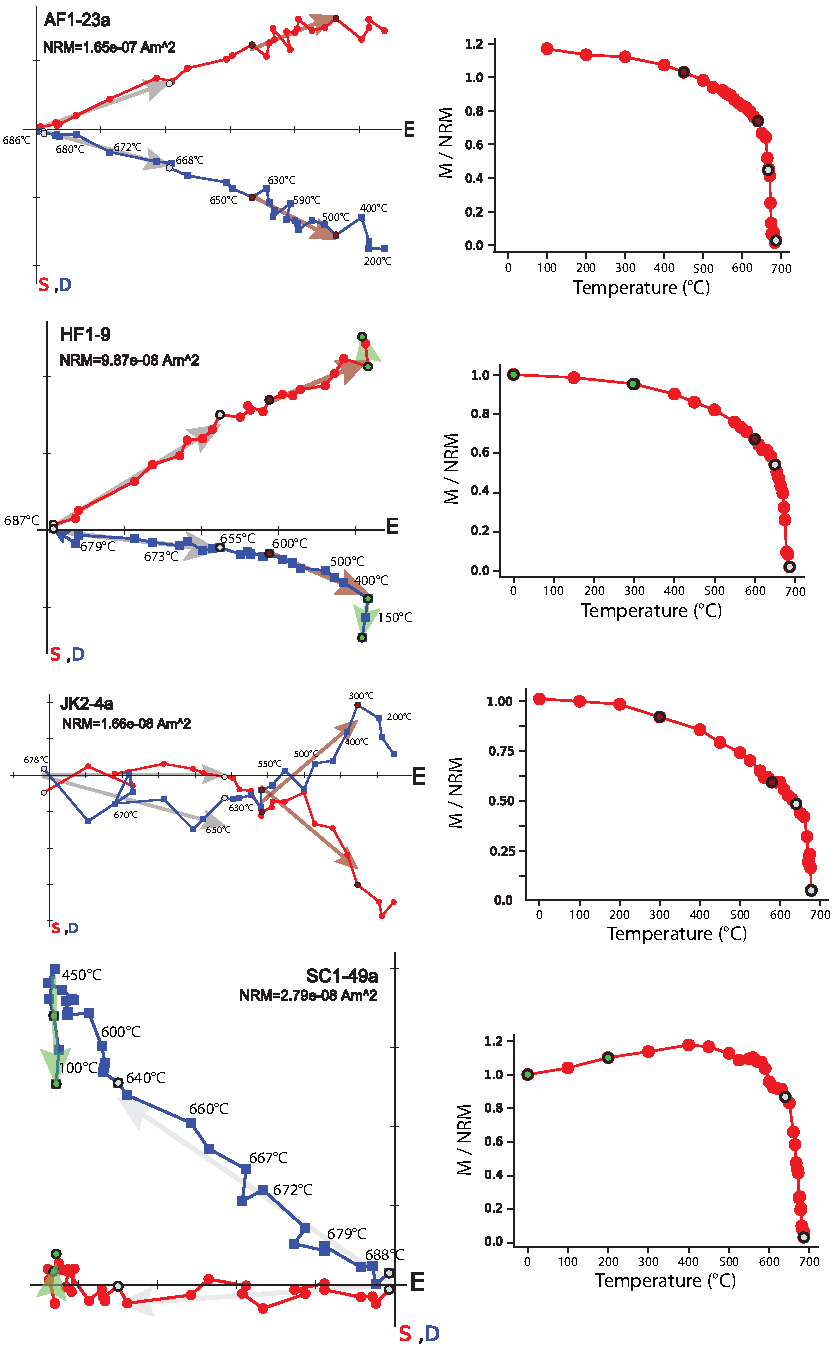
\includegraphics[width=0.6\textwidth]{figure/Zhang2024a/SI_orthogonal.pdf}
\caption[Representative orthogonal vector diagrams of demagnetization experiments for specimens from different stratigraphic sections of the Jacobsville Formation]{Representative orthogonal vector diagrams of demagnetization experiments for specimens from different stratigraphic sections of this study. An overprint component subparallel to the present day field direction in the study area is typically minimally present in siltstone to very fine-grained sandstone facies. This component shown in light green can be fit with a least-squares line in fine-grained facies. After the removal of the low-temperature component, a mid-temperature component typically unblocks through a wide range of temperature steps by up to $\sim$650\textdegree C. Finally, an origin-trending component with typically a shallower inclination than that of the mid-temperature component sharply unblocks through heating with smaller temperature intervals up toward the N\'eel temperature of hematite ($\sim$690\textdegree C). AF-Agate Falls section; HF-Hungarian side falls section near Dover Creek; JK-Hammel Creek section; SC-Snake Creek tributary section. M-magnetic moment; NRM-natural remanent magnetic moment. All diagrams are shown in tilt-corrected coordinates.}
\label{fig:SI_orthogonal}
\end{figure}

\begin{figure}
\centering
\includegraphics[width=0.5\textwidth]{figure/Zhang2024a/Jacobsville_pdf_directions.pdf}
\caption[Jacobsville Formation present day local field component]{Jacobsville present day local field directions. This present day overprint component is typically removed by $\sim$300\textdegree C.}
\label{fig:Jacobsville_pdf}
\end{figure}

\begin{figure}
\centering
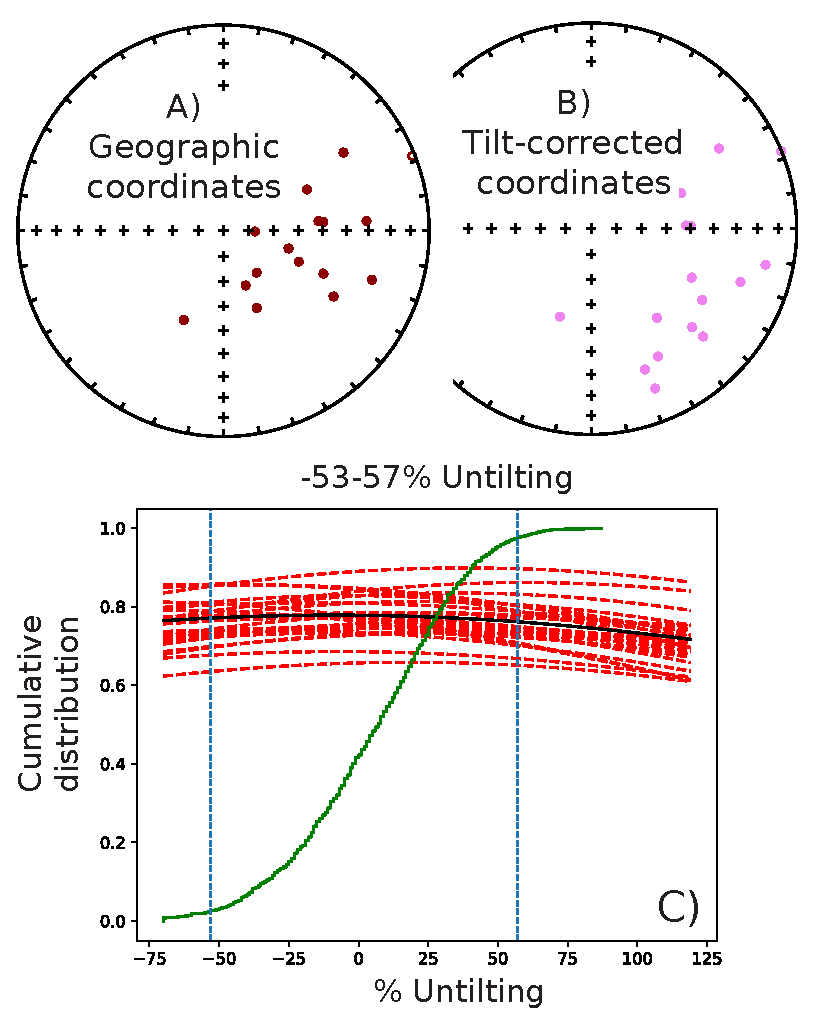
\includegraphics[width=0.9\textwidth]{figure/Zhang2024a/SI_hct_fold_test.pdf}
\caption[Paleomagnetic fold test at the Snake Creek tributary of the Jacobsville Formation]{Bootstrap paleomagnetic fold test \citep{Tauxe1994a} of the chemical remanent magnetization directions recorded by specimens from the nearly horizontal beds and moderately tilted beds at the Snake Creek tributary. Complete unfolding does not lie within the 95\% confidence limits of the test, consistent with the magnetization having been acquired syn- to post-folding.}
\label{fig:Jacobsville_hct_fold_test}
\end{figure}

\begin{figure}
\centering
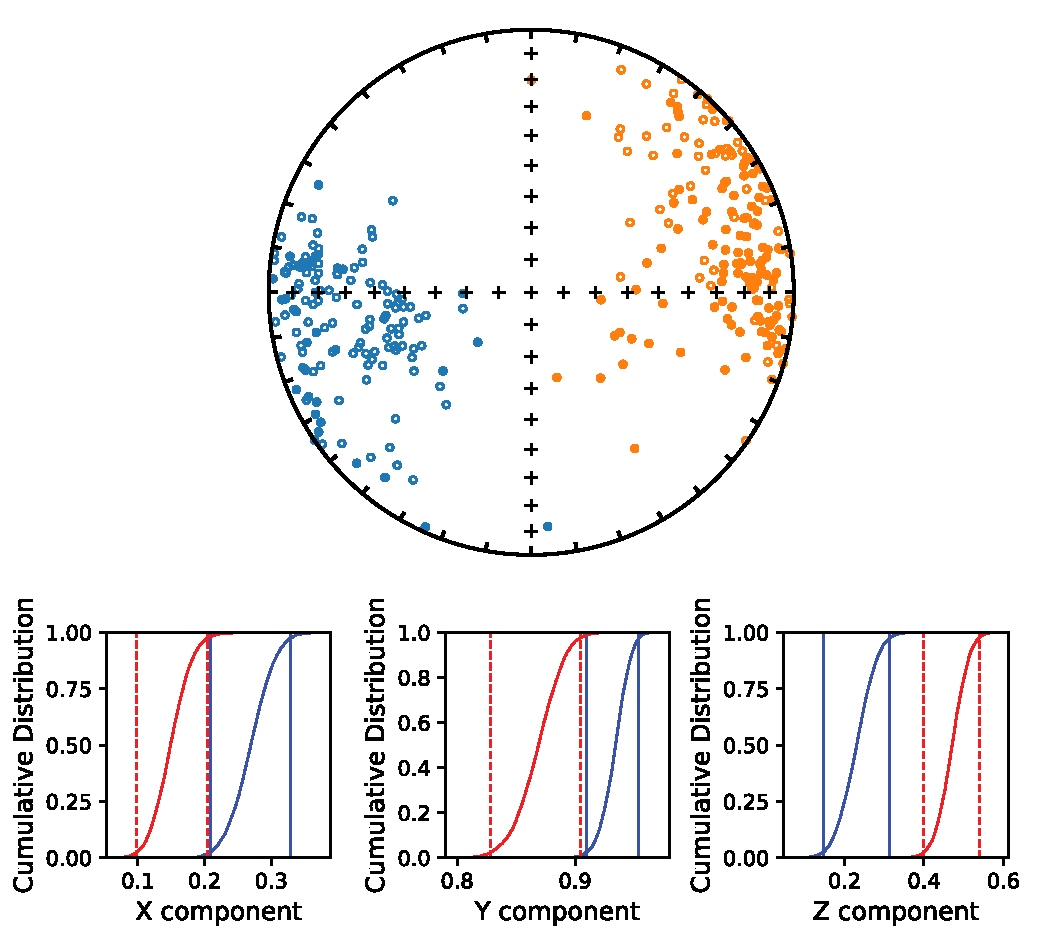
\includegraphics[width=0.9\textwidth]{figure/Zhang2024a/SI_reversal_test.pdf}
\caption[Paleomagnetic reversal test of the Jacobsville detrital remanence]{Jacobsville detrital remanence directions showing dual polarities plotted on an equal area stereonet plot. The directions do not pass a reversal test of \cite{McFadden1990a} as the angle between the mean directions is 15.9\textdegree\, larger than the critical angle of 7.5\textdegree. The directions also do not pass the bootstrap reversal test of \cite{Tauxe1991a}. }
\label{fig:Jacobsville_reversal_test}
\end{figure}

\begin{figure}
\centering
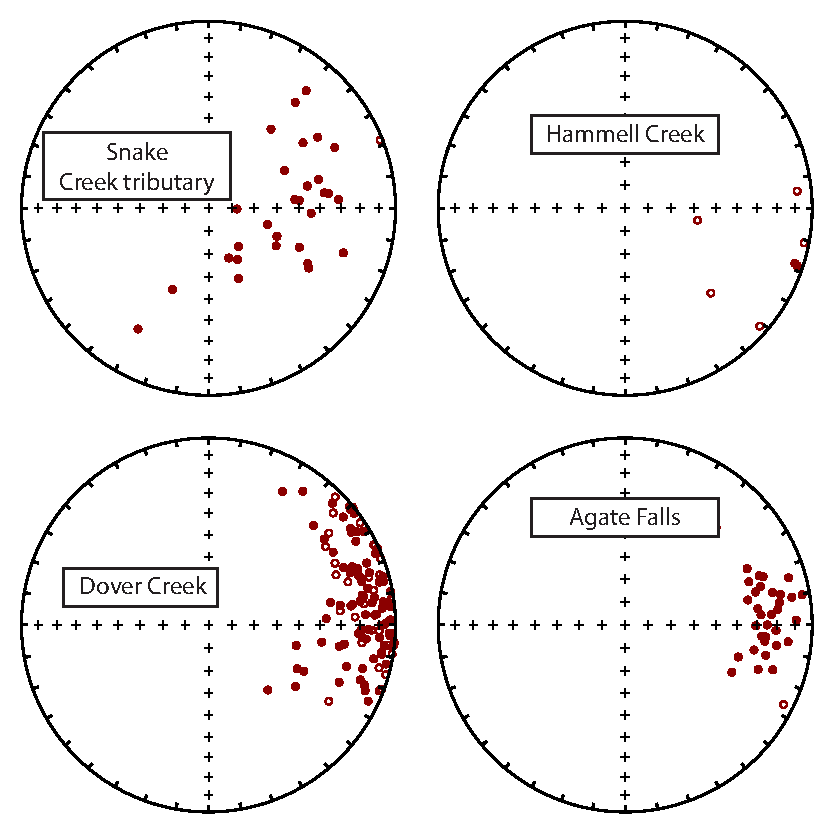
\includegraphics[width=0.9\textwidth]{figure/Zhang2024a/SI_hct.pdf}
\caption[Jacobsville Formation chemical remanence directions]{Jacobsville chemical remanence magnetization directions plotted by section. Samples collected from the Natural Wall section do not have interpretable chemical remanence component that can be fit with least-squares lines. All directions are plotted in geographic coordinates.}
\label{fig:Jacobsville_CRM}
\end{figure}

\begin{figure}
\centering
\includegraphics[width=0.75\textwidth]{figure/Zhang2024a/SI_Jacobsville_vs_Appalachian_poles.pdf}
\caption[Jacobsville detrital remanence pole position in context of Laurentia's paleomagnetic poles during Appalachian orogeny (ca. 460-260 Ma) as compiled in \cite{Torsvik2012a}]{Jacobsville detrital remanence Kent mean pole position and chemical remanence Fisher mean pole position (in geographic coordinates) plotted in context of Laurentia's paleomagnetic poles during Appalachian orogeny (ca. 460-260 Ma) as compiled in \cite{Torsvik2012a}. The mean chemical remanence pole position from the Snake Creek tributary section is plotted in context of the ca. 970-960 Ma poles developed by \cite{Brown2012a} from the Adirondack Highlands of the Grenville orogen. That this chemical remanence component failed a fold test (Figure \ref{fig:Jacobsville_hct_fold_test}) and yields a pole position that overlaps with the Grenville poles are consistent with the interpretation that the chemical remanence of the Jacobsville Formation at this locality was acquired  during the early Neoproterozoic, soon after Jacobsville deposition and deformation. That the Jacobsville DRM and CRM mean poles are distinct and far away from any of Laurentia's mid- to late-Paleozoic poles supports the interpretation that the Jacobsville detrital remanence magnetization was acquired during the Rigolet phase of the Grenvillian orogeny and the chemical remanence overprint was likely acquired soon after deposition as discussed in detail in the manuscript.}
\label{fig:Jacobsville_Appalachian}
\end{figure}

\begin{figure}
\centering
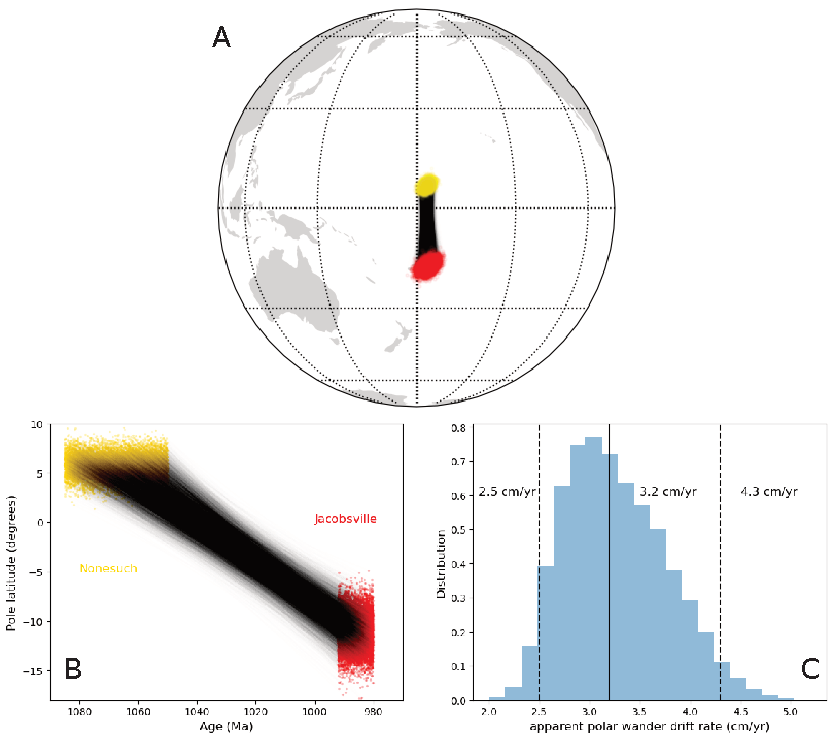
\includegraphics[width=0.9\textwidth]{figure/Zhang2024a/SI_Jacobsville_Nonesuch_rate.pdf}
\caption[Monte Carlo simulations of apparent polar wander rates implied by paleomagnetic and geochronologic data between the Nonesuch Formation and the Jacobsville Formation]{Monte Carlo simulations of apparent polar wander rates implied by paleomagnetic and geochronologic data between the Nonesuch Formation and the Jacobsville Formation. (A) The gold and red points are 10,000 simulated Kent distribution mean paleomagnetic poles for the Nonesuch Formation and Jacobsville Formation, respectively. The simulated poles are connected by gray lines which represent the apparent polar wander great circle paths. (B) The points color-coded in the same way as in (A) show the simulated paleomagnetic pole latitudes plotted against their simulated pole ages using uniform distributions. The points are connected by gray lines which represent the simulated pole latitudinal motion. The histogram on the right shows all 10,000 of the simulated rates that yield the labeled 2.5 percentile value of 2.5 cm/yr, median value of 3.2 cm/yr and 97.5 percentile value of 4.3 cm/yr.}
\label{fig:Jacobsville_Nonesuch_rate}
\end{figure}

\begin{sidewaystable}
\tiny
\caption[Compilation of Laurentian paleomagnetic poles]{\scriptsize Compilation of up-to-date Keweenawan Track paleomagnetic poles and ca. 780-720 Ma Laurentian paleomagnetic poles. }
\begin{tabular}{p{4cm}lllp{4cm}p{1.3cm}p{1.2cm}p{1.2cm}p{4cm}}

\hline
\multicolumn{9}{c}{Compilation of Fisher mean paleomagnetic poles}                                                                                                                                                                                        \\ \hline
Pole                                                       & Pole lat & Pole lon & A95  & Pole reference                                                         & AgeNominal & AgeLower & AgeUpper & Age reference                                       \\
Osler reverse (lower)                                      & 40.9     & 218.6    & 4.8  & \cite{Swanson-Hysell2014a}                                           & 1108       & 1105.15  & 1110     & \cite{Davis1985a, Swanson-Hysell2019a}               \\
Osler reverse (upper)                                      & 42.3     & 203.4    & 3.7  & \cite{Halls1974a, Davis1985a, Swanson-Hysell2014a} & 1105.15    & 1104.82  & 1105.48  & \cite{Swanson-Hysell2019a}                       \\
Mamainse lower reversed 1                                  & 49.5     & 227      & 5.3  & \cite{Swanson-Hysell2014b}                                           & 1109       & 1106     & 1112     & As discussed in \cite{Swanson-Hysell2019a}         \\
Mamainse lower reversed 2                                  & 37.5     & 205.2    & 4.5  & \cite{Swanson-Hysell2014b}                                                  & 1105       & 1100.4   & 1109     & \cite{Swanson-Hysell2014b}                              \\
Mamainse lower normal and upper reversed                   & 36.1     & 189.7    & 4.9  & \cite{Swanson-Hysell2014b}                                                  & 1100.36    & 1100.1   & 1100.61  & \cite{Swanson-Hysell2014b}                               \\
Mamainse upper normal                                      & 31.2     & 183.2    & 2.5  & \cite{Swanson-Hysell2014b}                                                  & 1094       & 1090     & 1100     & As discussed in S\cite{Swanson-Hysell2019a}            \\
Grand Portage Basalts                                      & 46       & 201.7    & 6.8  & \cite{Books1968a, Tauxe2009a}                                    & 1106       & 1105.28  & 1108     & \cite{Swanson-Hysell2019a}                         \\
North Shore Volcanic Group (upper NE   sequence)           & 31.1     & 181.7    & 4.2  & \cite{Books1972a, Tauxe2009a}                                    & 1095       & 1092     & 1098     & \cite{Davis1997a, Fairchild2017a}       \\
North Shore Volcanic Group (upper SW   sequence)           & 36.9     & 179.3    & 2.1  & \cite{Tauxe2009a, Swanson-Hysell2019a}                   & 1096.18    & 1093.94  & 1096.75  & \cite{Swanson-Hysell2019a}                        \\
Schroeder Lutsen Basalts                                   & 28.3     & 187.6    & 2.5  & \cite{Books1972a, Tauxe2009a, Fairchild2017a}            & 1090       & 1085     & 1091.5   & \cite{Fairchild2017a}                               \\
Portage Lake Volcanics                                     & 27.5     & 182.5    & 2.3  & \cite{Books1972a, Hnat2006a}                                         & 1092.51    & 1091.59  & 1093.37  & \cite{Swanson-Hysell2019a}                    \\
Lake Shore Traps                                           & 22.2     & 180.8    & 4.5  & \cite{Diehl1994a}                                                     & 1085.47    & 1084     & 1091     & \cite{Fairchild2017a, Swanson-Hysell2019a}    \\
Siemens Creek Volcanics                                    & 45.8     & 214      & 9.2  & \cite{Palmer1986a}                                                 & 1108       & 1105     & 1111     & \cite{Davis1997a}                               \\
Michipicoten Island Formation                              & 17       & 174.7    & 4.4  & \cite{Palmer1987a, Fairchild2017a}                        & 1083.95    & 1083.52  & 1084.39  & \cite{Fairchild2017a}                           \\
Freda Formation                                            & 2.2      & 179      & 4.2  & \cite{Henry1977a}                                                     & 1070       & 1060     & 1083.5   & As discussed in \cite{Swanson-Hysell2019a}            \\
Haliburton Intrusions                                      & -36.2    & 141.7    & 6.0  & \cite{Buchan1976a}                          & 1015       & 1000     & 1030     & \cite{Warnock2000a}                                          \\
Adirondack Highlands gneiss                                & -19      & 148.7    & 11.2 & \cite{Brown2012a}                                                &            &          &          &                                                     \\
Adirondack Highlands anorthositic rocks                    & -25.2    & 143.4    & 12.9 & \cite{Brown2012a}                                                &            &          &          &                                                     \\
Adirondack Highlands granites                              & -28.5    & 131.7    & 7.1  & \cite{Brown2012a}                                                &            &          &          &                                                     \\
Franklin large igneous province   Victoria/Mainland/Baffin & 6.7      & 162.1    & 3    & \cite{Denyszyn2009a}                                                   & 716.33     & 715.79   & 716.87   &                                                     \\
Combo Carbon Butte–Awatubi                                 & 14.2     & 163.8    & 3.5  & \cite{Eyster2019a}                                                   & 751        & 743.4    & 758.6    &                                                     \\
Carbon Canyon                                              & -0.5     & 166      & 9.7  & compilation by \cite{Eyster2019a}                                    & 757        & 750.2    & 763.8    &                                                     \\
UMG Group 3                                                & 4.9      & 160.6    & 3.2  & compilation by \cite{Eyster2019a}                                    & 755        &          &          & As discussed in \cite{Eyster2019a}                \\
Nankoweap                                                  & -10      & 163      & 4.9  & \cite{Weil2003a}                                                     & 782        &          &          & As discussed in Eyster et al., 2020                 \\
UMG Group 2                                                & -5.8     & 158.7    & 2.7  & compilation by \cite{Eyster2019a}                                    & 760        &          &          & As discussed in Eyster et al., 2021                 \\
UMG Group 1                                                & 3        & 163.5    & 3.2  & compilation by \cite{Eyster2019a}                                    & 766        &          &          & As discussed in Eyster et al., 2022                 \\
Gunbarrel mean                                             & 9.1      & 138.2    & 11.7 & \cite{Eyster2019a}                                                   & 774.93     & 774.39   & 775.47   &                                                    
\end{tabular}
\label{tab:pole_compilation}
\end{sidewaystable}

\clearpage

\begin{sidewaystable}
\begin{scriptsize}
\begin{tabular}{p{1.5cm}p{1cm}p{1cm}p{1cm}p{1cm}p{1cm}p{1cm}p{1cm}p{1cm}p{1cm}p{1cm}p{1cm}p{1cm}p{2cm}}
\hline
\multicolumn{14}{c}{Compilation of Kent mean paleomagnetic poles}                                                                                                                                                                                           \\ \hline 
Pole                  & Pole lat & Pole lon & Major axis lat & Major axis lon & Major axis magnitude & Minor axis lat & Minor axis lon & Minor axis magnitude & Pole reference         & Age Nominal & Age Lower & Age Upper & Age reference                                       \\
Nonesuch Formation    & 6.6      & 182.9    & 27.6           & 280.2          & 2.8                  & 41.6           & 87             & 2                    & \cite{Slotznick2023a} & 1080       & 1070     & 1083.5   & As discussed in \cite{Swanson-Hysell2019a}         \\
Jacobsville Formation & 16.9    & 183.4    & 45.2           & 255.5          & 4.1                    & 39.9           & 108.1          & 3.1                  & this study             & 990        & 985      & 992     & \cite{Hodgin2022a}; as discussed in the manuscript
\end{tabular}
\end{scriptsize}
\end{sidewaystable}

\clearpage



\chapter[Supporting Information for ``Paleomagnetism of the southwest Laurentia large igneous province and Cardenas Basalt: pulsed magmatism during rapid late Mesoproterozoic plate motion"][Supporting Information--SWLLIP]{Supporting Information for ``Paleomagnetism of the southwest Laurentia large igneous province and Cardenas Basalt: pulsed magmatism during rapid late Mesoproterozoic plate motion"}

\begin{figure}
\centering
\includegraphics[width=\textwidth]{figure/Zhang2024b/Cardenas_Unkar_geochem_major.pdf}
\caption[Major element geochemical data of the Cardenas Basalt and diabase intrusions in the Unkar Group.]{Total alkali-silica diagram of the Cardenas Basalt and mafic intrusions within the Unkar Group. The sills and dikes typically have lower silica content (basalt) than the Cardenas Basalt (basaltic trachy-andesite). Data for the Cardenas Basalt are from \cite{Hendricks1989a} and \cite{Larson1994a}. Data for the intrusions are from \cite{Hendricks1989a}.}
\label{fig:geochem_major}
\end{figure}

\begin{figure}
\noindent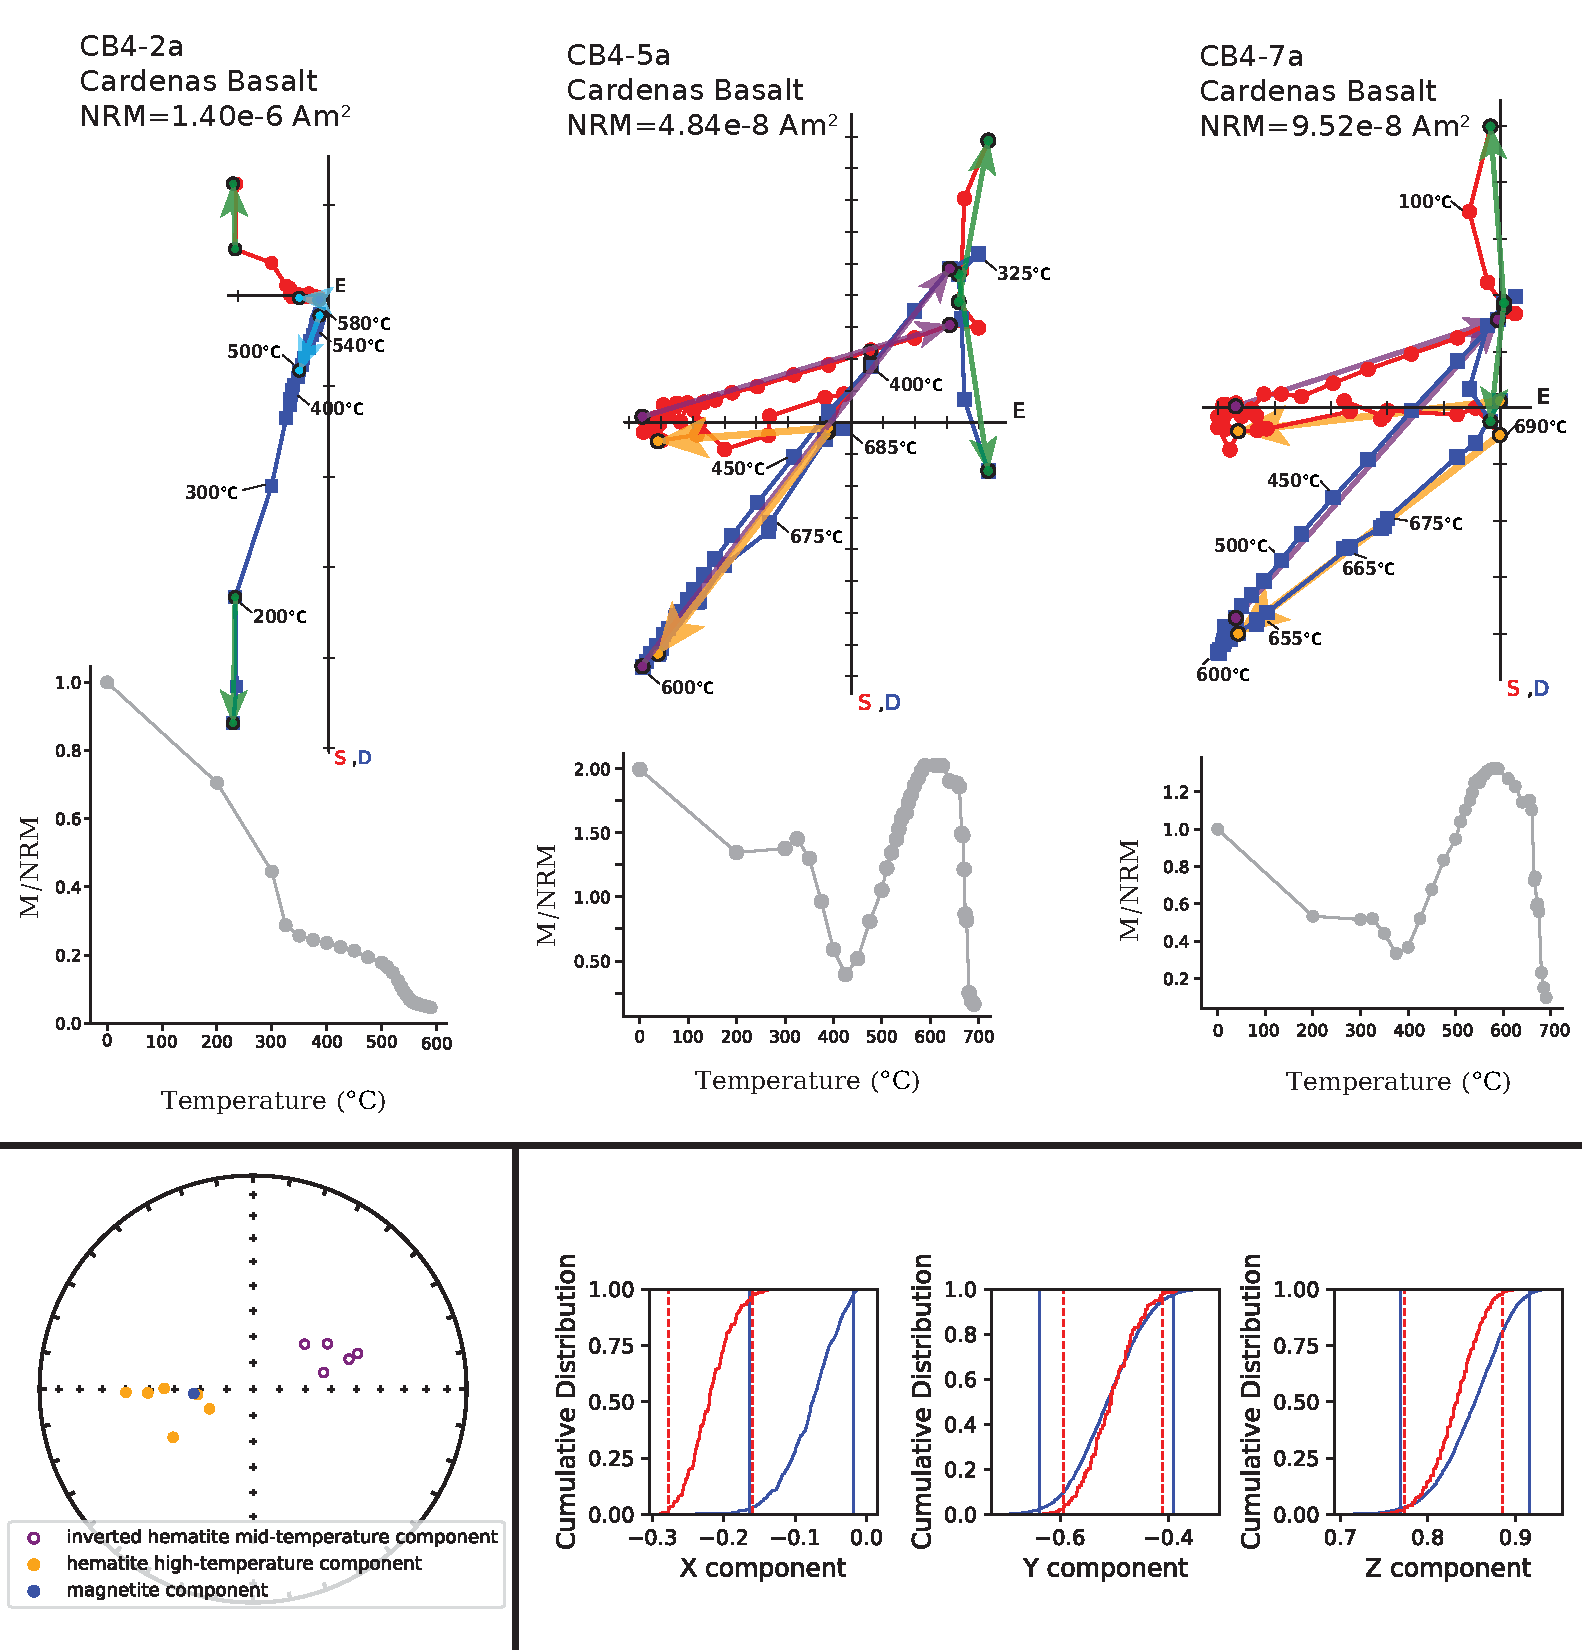
\includegraphics[width=5.8 in]{figure/Zhang2024b/SI_CB4.pdf}
\caption[Paleomagnetic data of Cardenas Basalt lava flow site CB4.]{\footnotesize Top panel: Thermal demagnetization data of paleomagnetic specimens collected near the bottom of lava flow CB4. Specimen CB4-2a has a demagnetization behavior similar to other lava flows--after the removal of the present day local field overprint, an origin-trending magnetite-carrying characteristic component unblocks up to 580\textdegree C. However, for all other specimens, after the removal of the present day local field overprint by $\sim$300\textdegree C (green vector), their total magnetic moments typically increase as the thermal demagnetization approaches $\sim$600\textdegree C. This mid-temperature component is followed by an origin-trending decay approaching the N\`eel temperature of hematite. Bottom panel: Bootstrap reversal test \citep{Tauxe1991a} of the mid-temperature and high-temperature remanence component of CB4. The directions pass the bootstrap reversal test and \cite{McFadden1990a} reversal test of  with a `C' classification. The high-temperature component that unblocks sharply near the hematite N\`eel temperature has the same polarity with titanomagnetite carried directions in other Cardenas Basalt flows. This similarity is consistent with the hematite forming from oxidation soon after eruption \citep{Haggerty1967a}. A likely origin of the antipodal component is that it is a self-reversed chemical remanent magnetization held by fine-grained hematite that formed as a result of inversion of maghemite precursors \citep{Hedley1968a, McClelland1987a, McClelland1993a, Swanson-Hysell2011a}. This self-reversal behavior is more likely than one that involves the reversal of the geomagnetic field after the emplacement of the CB4 lava flow. No reversed direction is observed in the adjacent lava flows and previous compilations of paleomagnetic data during this time suggest that the Cardenas lava flows were emplaced during a normal-polarity superchron \citep{Swanson-Hysell2019a, Driscoll2016b}.}
\label{fig:CB4_reversal_test}
\end{figure}

\begin{figure}
\noindent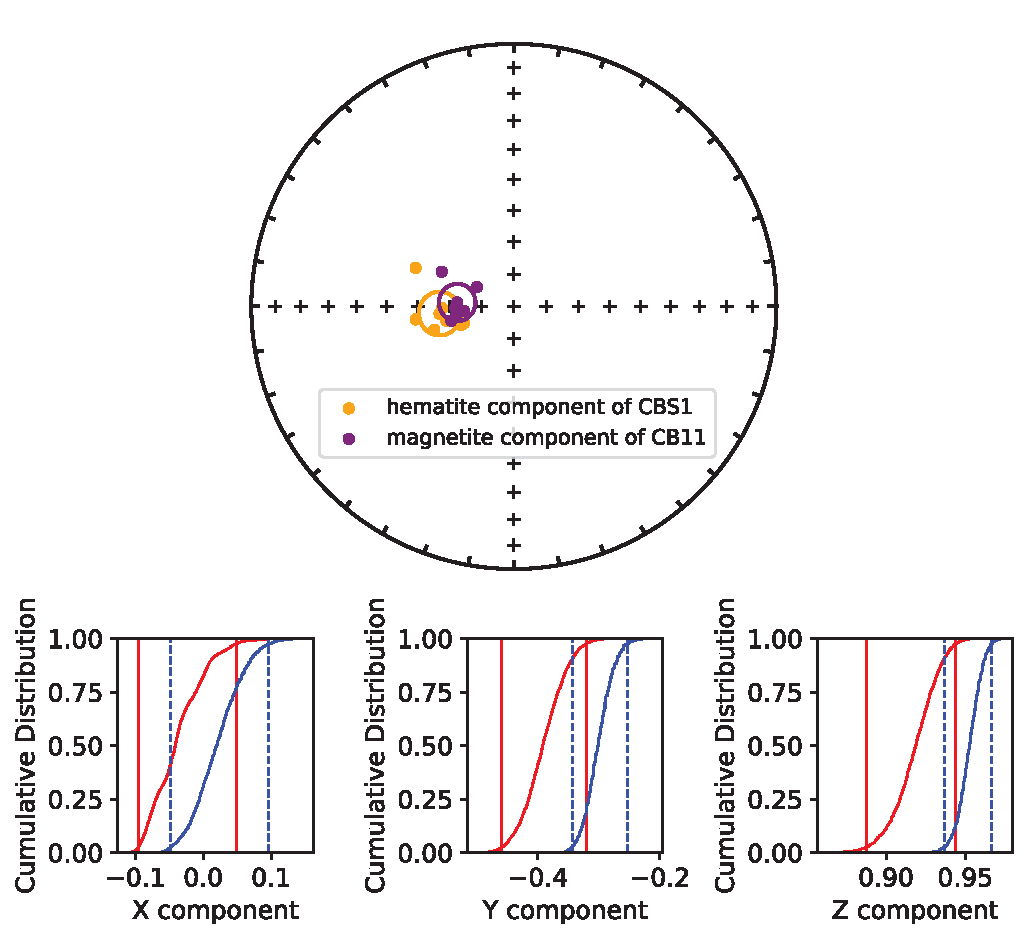
\includegraphics[width=5.8 in]{figure/Zhang2024b/SI_CBS1_CB11.pdf}
\caption[Paleomagnetic data of Cardenas Basalt lava flow site CB11 and the interflow sandstone site CBS1 below CB11.]{Top: Equal area plot showing the hematite magnetization specimen directions (orange) of the interflow sandstone CBS1 which is stratigraphically below the CB11 lava flow, whose magnetite magnetization directions are shown in purple. Bottom: Bootstrap common mean test of \cite{Tauxe1991a} between the specimens directions of the sandstone and the lava flow show a positive result. The specimen directions also passes a common mean test of \cite{McFadden1990a} with a `B' classification and have a positive support for sharing a common mean based on the Bayesian approach of \cite{Heslop2023a}.}
\label{fig:SI_CBS1_CB11}
\end{figure}


\begin{figure}
\noindent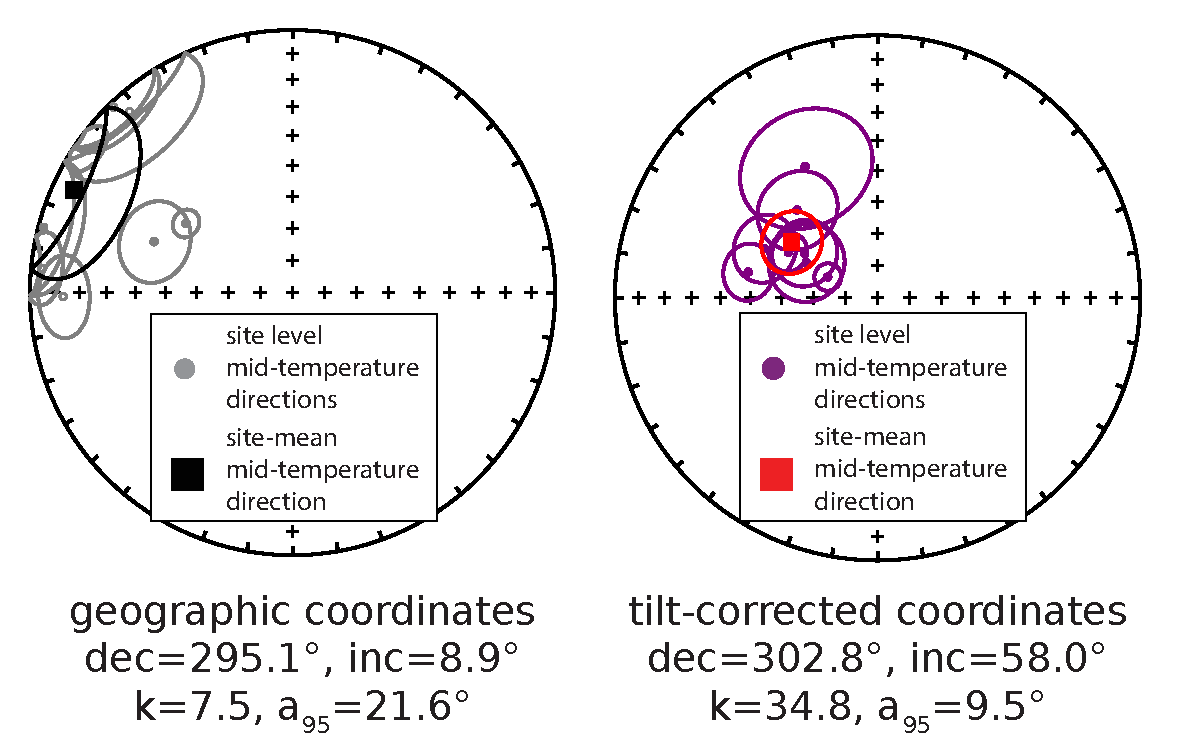
\includegraphics[width=5.8 in]{figure/Zhang2024b/SI_tilt_test.pdf}
\caption[Death Valley diabase sill paleomagnetic tilt test]{Equal area plots showing the site-level directions and site-mean directions of the Death Valley diabase sills that yielded coherent within-site thermal demagnetization results in both geographic coordinates (left) and tilt-corrected coordinates (right). The site-mean direction in geographic coordinates is dec=295.1\textdegree, inc=8.9\textdegree, n=8, k=7.5, a$_{95}$=21.6\textdegree. The site-mean direction in tilt-corrected coordinates is dec=302.8\textdegree, inc=58.0\textdegree, k=34.8, a$_{95}$=9.5\textdegree. Applying tilt correction to the sills significantly improves the grouping of the site level directions. }
\label{fig:DV_tilt_test}
\end{figure}

\begin{figure}
\noindent\includegraphics[width=5.8 in]{figure/Zhang2024b/SI_Cardenas_QQ.png}
\caption[Cardenas Basalt VGPs Fisher distribution test]{Fisher quantile-quantile \cite{Fisher1987a} test of the distribution of the site level virtual geomagnetic poles of the Cardenas Basalt lava flows. The results show that the null hypothesis that the VGPs are Fisher-distributed cannot be rejected.}
\label{fig:Cardenas_QQ}
\end{figure}

\begin{figure}
\centering
\includegraphics[width=0.7\textwidth]{figure/Zhang2024b/Larson1994a_trace_elements.pdf}
\caption[Trace element geochemistry data of the Cardenas Basalt and the Hance sill.]{Trace element geochemistry data from \cite{Larson1994a}. The elemental abundance of the interior of the Hance sill is similar to that of the Cardenas Basalt lavas. Virtual geomagnetic poles developed from the Hance sill, Hance dike, and another undated sill in Red Canyon adjacent to Hance rapids plot closer to those of the Cardenas Basalt than the dated ca. 1098 Ma poles as shown in the main text. These data are consistent with the interpretation that the intrusions near Hance rapids are feeders to the Cardenas Basalt.}
\label{fig:trace_elements}
\end{figure}


\begin{sidewaystable}
\tiny
\caption[Compilation of paleomagnetic data developed from mafic sills in central Arizona by \cite{Harlan1993a} and \cite{Donadini2011a}.]{\scriptsize Compilation of paleomagnetic data collected from mafic sills in central Arizona by \cite{Harlan1993a} and \cite{Donadini2011a}. The study of \cite{Donadini2011a} revisited some field areas of \cite{Harlan1993a} and resampled some diabase sills in the earlier study. However, the determination of individual cooling units was not clear in \cite{Donadini2011a}. We compiled data from both studies with a focus on distinguishing individual paleomagnetic sites as distinct cooling units based on geographic and paleomagnetic information provided in the original publications. Data rejected by the original authors are not included. Original ``site" level data with better Fisher statistics (higher concentration parameter k values) are preferentially used in cases where repeat sampling of the same cooling unit is interpreted to have happened. We interpret site GD12 and GD13 of \cite{Harlan1993a} are the same as site OD in \cite{Donadini2011a} and thus recalculated mean statistics. dir\_dec---declination; dir\_inc--- inclination; k---kappa concentration parameter of the site mean direction; a$_{95}$---95\% confidence angle of site mean direction; n---number of samples included in each site; N---number of sites used in calculating the mean statistics by polarity; plat/Plat---pole latitude; plon/Plon---pole longitude. The site level pole locations are recalculating using the directions and site location information provided in the original studies.}
\begin{tabular}{p{3cm}p{1cm}p{1cm}p{1cm}p{1cm}p{1cm}p{1.2cm}p{1cm}p{3cm}p{1cm}p{1cm}p{1cm}}

site                   & dir\_dec & dir\_inc & k     & a95  & n  & slon    & slat  & pole reference                      & plon  & plat  & polarity \\
\hline 
GD01-02                & 279.2    & 57       &       &      &    & 249.5   & 33.7  & Harlan, 1993                        & 188.7 & 26.4  & N        \\
GD03                   & 285.3    & 51.4     & 165   & 3.6  & 11 & 249.5   & 33.8  & Harlan, 1993                        & 180.7 & 28.8  & N        \\
GD04                   & 295.5    & 56.6     & 81.9  & 7.7  & 7  & 249.5   & 33.8  & Harlan, 1993                        & 182.9 & 38.4  & N        \\
GD05                   & 283.2    & 26       & 108.5 & 5.8  & 7  & 249.5   & 33.8  & Harlan, 1993                        & 163.9 & 18.4  & N        \\
GD06-07                & 282.8    & 48.9     &       &      &    & 249.3   & 33.5  & Harlan, 1993                        & 179.3 & 25.8  & N        \\
GD08                   & 318      & 61.2     & 56.1  & 5.6  & 13 & 249.3   & 33.5  & Harlan, 1993                        & 186.8 & 56.1  & N        \\
GD09                   & 299.2    & 53.8     & 21.1  & 11.5 & 9  & 249.3   & 33.5  & Harlan, 1993                        & 178.3 & 40.3  & N        \\
GD10                   & 267.5    & 38.2     & 421.5 & 3.3  & 6  & 249.3   & 33.5  & Harlan, 1993                        & 178.7 & 9.7   & N        \\
GD17                   & 285.9    & 17.1     & 34.5  & 8.3  & 10 & 249.1   & 33.6  & Harlan, 1993                        & 157.7 & 18    & N        \\
GD18-20                & 339.6    & 36.3     &       &      &    & 249.2   & 33.5  & Harlan, 1993                        & 128   & 67.5  & N        \\
GD22                   & 270.1    & 40.4     & 120.3 & 5.1  & 8  & 249.5   & 33.8  & Harlan, 1993                        & 178.9 & 12.7  & N        \\
GD24                   & 297.9    & 58.5     & 168   & 4    & 9  & 249.5   & 33.8  & Harlan, 1993                        & 184.8 & 40.8  & N        \\
GD29                   & 306.9    & 66.4     & 678.5 & 2    & 9  & 249.4   & 33.6  & Harlan, 1993                        & 197.2 & 48.2  & N        \\
GD30                   & 264.1    & 33.4     & 157.6 & 5.4  & 6  & 249.4   & 33.6  & Harlan, 1993                        & 177.8 & 5.3   & N        \\
DF                     & 332.6    & 69.4     & 145.1 & 3.5  & 13 & 249.3   & 33.5  & Donadini et al., 2011               & 212.7 & 62.5  & N        \\
DG                     & 266.2    & 34.4     & 58.7  & 8    & 7  & 249.4   & 33.6  & Donadini et al., 2011               & 176.9 & 7.4   & N        \\
DJ                     & 281.9    & 52.8     & 325.5 & 2.9  & 9  & -110.48 & 33.65 & Donadini et al., 2011               & 182.8 & 26.7  & N        \\
KD                     & 293.8    & 13.4     & 142.3 & 3.3  & 14 & -110.97 & 33.89 & Donadini et al., 2011               & 151.2 & 23.5  & N        \\
MD                     & 277.2    & 50.7     & 110.4 & 4.2  & 12 & -110.98 & 33.87 & Donadini et al., 2011               & 182.9 & 22.2  & N        \\
GD12\_GD13\_OD         & 280.8    & 45.7     & 313.7 & 7    &    & -110.98 & 33.81 & Harlan, 1993; Donadini et al., 2011 & 177.6 & 23    & N        \\
GD11                   & 115.3    & -69.9    & 173.7 & 4.2  & 8  & -110.96 & 33.75 & Harlan, 1993                        & 24.3  & -41   & R        \\
GD15-27                & 224.9    & -73.7    &       &      &    & -110.5  & 33.8  & Harlan, 1993                        & 103.8 & -50.9 & R        \\
BD                     & 137.6    & -74      & 66.1  & 8.2  & 7  & -110.61 & 33.61 & Donadini et al., 2011               & 36.5  & -52   & R        \\
WD                     & 199.2    & -71      & 92.1  & 3.1  & 24 & -110.69 & 33.55 & Donadini et al., 2011               & 95    & -64.4 & R        \\
                       &          &          &       &      &    &         &       &                                     &       &       &          \\
\hline 
                       & dir\_dec & dir\_inc & k     & a95  & N  & Plon    & Plat  & A95                                 &       &       &          \\
\hline 
normal polarity mean   & 287.6    & 47.4     & 14.4  & 8.5  & 20 & 177.4   & 30.6  & 8.9                                 &       &       &          \\
reversed polarity mean & 167.4    & -77      & 31.8  & 16.6 & 4  & 239.9   & 57.5  & 30.6                                &       &       &         
\end{tabular}

\end{sidewaystable}

\clearpage







\end{document}